\documentclass[twoside]{book}

% Packages required by doxygen
\usepackage{calc}
\usepackage{doxygen}
\usepackage{graphicx}
\usepackage[utf8]{inputenc}
\usepackage{makeidx}
\usepackage{multicol}
\usepackage{multirow}
\usepackage{textcomp}
\usepackage[table]{xcolor}

% NLS support packages
Portuguese
% Font selection
\usepackage[T1]{fontenc}
\usepackage{mathptmx}
\usepackage[scaled=.90]{helvet}
\usepackage{courier}
\usepackage{amssymb}
\usepackage{sectsty}
\renewcommand{\familydefault}{\sfdefault}
\allsectionsfont{%
  \fontseries{bc}\selectfont%
  \color{darkgray}%
}
\renewcommand{\DoxyLabelFont}{%
  \fontseries{bc}\selectfont%
  \color{darkgray}%
}

% Page & text layout
\usepackage{geometry}
\geometry{%
  a4paper,%
  top=2.5cm,%
  bottom=2.5cm,%
  left=2.5cm,%
  right=2.5cm%
}
\tolerance=750
\hfuzz=15pt
\hbadness=750
\setlength{\emergencystretch}{15pt}
\setlength{\parindent}{0cm}
\setlength{\parskip}{0.2cm}
\makeatletter
\renewcommand{\paragraph}{%
  \@startsection{paragraph}{4}{0ex}{-1.0ex}{1.0ex}{%
    \normalfont\normalsize\bfseries\SS@parafont%
  }%
}
\renewcommand{\subparagraph}{%
  \@startsection{subparagraph}{5}{0ex}{-1.0ex}{1.0ex}{%
    \normalfont\normalsize\bfseries\SS@subparafont%
  }%
}
\makeatother

% Headers & footers
\usepackage{fancyhdr}
\pagestyle{fancyplain}
\fancyhead[LE]{\fancyplain{}{\bfseries\thepage}}
\fancyhead[CE]{\fancyplain{}{}}
\fancyhead[RE]{\fancyplain{}{\bfseries\leftmark}}
\fancyhead[LO]{\fancyplain{}{\bfseries\rightmark}}
\fancyhead[CO]{\fancyplain{}{}}
\fancyhead[RO]{\fancyplain{}{\bfseries\thepage}}
\fancyfoot[LE]{\fancyplain{}{}}
\fancyfoot[CE]{\fancyplain{}{}}
\fancyfoot[RE]{\fancyplain{}{\bfseries\scriptsize Gerado em Quarta, 15 de Junho de 2016 17\-:35\-:20 para Projeto Final M\-P por Doxygen }}
\fancyfoot[LO]{\fancyplain{}{\bfseries\scriptsize Gerado em Quarta, 15 de Junho de 2016 17\-:35\-:20 para Projeto Final M\-P por Doxygen }}
\fancyfoot[CO]{\fancyplain{}{}}
\fancyfoot[RO]{\fancyplain{}{}}
\renewcommand{\footrulewidth}{0.4pt}
\renewcommand{\chaptermark}[1]{%
  \markboth{#1}{}%
}
\renewcommand{\sectionmark}[1]{%
  \markright{\thesection\ #1}%
}

% Indices & bibliography
\usepackage{natbib}
\usepackage[titles]{tocloft}
\setcounter{tocdepth}{3}
\setcounter{secnumdepth}{5}
\makeindex

% Hyperlinks (required, but should be loaded last)
\usepackage{ifpdf}
\ifpdf
  \usepackage[pdftex,pagebackref=true]{hyperref}
\else
  \usepackage[ps2pdf,pagebackref=true]{hyperref}
\fi
\hypersetup{%
  colorlinks=true,%
  linkcolor=blue,%
  citecolor=blue,%
  unicode%
}

% Custom commands
\newcommand{\clearemptydoublepage}{%
  \newpage{\pagestyle{empty}\cleardoublepage}%
}


%===== C O N T E N T S =====

\begin{document}

% Titlepage & ToC
\hypersetup{pageanchor=false}
\pagenumbering{roman}
\begin{titlepage}
\vspace*{7cm}
\begin{center}%
{\Large Projeto Final M\-P }\\
\vspace*{1cm}
{\large Gerado por Doxygen 1.8.6}\\
\vspace*{0.5cm}
{\small Quarta, 15 de Junho de 2016 17:35:20}\\
\end{center}
\end{titlepage}
\clearemptydoublepage
\tableofcontents
\clearemptydoublepage
\pagenumbering{arabic}
\hypersetup{pageanchor=true}

%--- Begin generated contents ---
\chapter{Índice da hierarquia}
\section{Hierarquia de classes}
Esta lista de heranças está organizada, dentro do possível, por ordem alfabética\-:\begin{DoxyCompactList}
\item \contentsline{section}{std\-:\-:tr1\-:\-:gtest\-\_\-internal\-:\-:Add\-Ref$<$ T $>$}{\pageref{structstd_1_1tr1_1_1gtest__internal_1_1AddRef}}{}
\item \contentsline{section}{std\-:\-:tr1\-:\-:gtest\-\_\-internal\-:\-:Add\-Ref$<$ T \& $>$}{\pageref{structstd_1_1tr1_1_1gtest__internal_1_1AddRef_3_01T_01_6_01_4}}{}
\item \contentsline{section}{testing\-:\-:internal\-:\-:Add\-Reference$<$ T $>$}{\pageref{structtesting_1_1internal_1_1AddReference}}{}
\item \contentsline{section}{testing\-:\-:internal\-:\-:Add\-Reference$<$ T \& $>$}{\pageref{structtesting_1_1internal_1_1AddReference_3_01T_01_6_01_4}}{}
\item \contentsline{section}{Aresta}{\pageref{structAresta}}{}
\item \contentsline{section}{testing\-:\-:internal\-:\-:Assert\-Helper}{\pageref{classtesting_1_1internal_1_1AssertHelper}}{}
\item \contentsline{section}{testing\-:\-:Assertion\-Result}{\pageref{classtesting_1_1AssertionResult}}{}
\item \contentsline{section}{testing\-:\-:internal\-:\-:bool\-\_\-constant$<$ bool\-\_\-value $>$}{\pageref{structtesting_1_1internal_1_1bool__constant}}{}
\begin{DoxyCompactList}
\item \contentsline{section}{testing\-:\-:internal\-:\-:is\-\_\-pointer$<$ T $>$}{\pageref{structtesting_1_1internal_1_1is__pointer}}{}
\item \contentsline{section}{testing\-:\-:internal\-:\-:is\-\_\-pointer$<$ T $\ast$ $>$}{\pageref{structtesting_1_1internal_1_1is__pointer_3_01T_01_5_01_4}}{}
\end{DoxyCompactList}
\item \contentsline{section}{testing\-:\-:internal\-:\-:bool\-\_\-constant$<$ Implicitly\-Convertible$<$ const T $\ast$, const \-:\-:Protocol\-Message $\ast$ $>$\-:\-:value$\vert$$\vert$\-Implicitly\-Convertible$<$ const T $\ast$, const \-:\-:proto2\-:\-:Message $\ast$ $>$\-:\-:value $>$}{\pageref{structtesting_1_1internal_1_1bool__constant}}{}
\begin{DoxyCompactList}
\item \contentsline{section}{testing\-:\-:internal\-:\-:Is\-A\-Protocol\-Message$<$ T $>$}{\pageref{structtesting_1_1internal_1_1IsAProtocolMessage}}{}
\end{DoxyCompactList}
\item \contentsline{section}{std\-:\-:tr1\-:\-:gtest\-\_\-internal\-:\-:By\-Ref$<$ T $>$}{\pageref{structstd_1_1tr1_1_1gtest__internal_1_1ByRef}}{}
\item \contentsline{section}{std\-:\-:tr1\-:\-:gtest\-\_\-internal\-:\-:By\-Ref$<$ T \& $>$}{\pageref{structstd_1_1tr1_1_1gtest__internal_1_1ByRef_3_01T_01_6_01_4}}{}
\item \contentsline{section}{testing\-:\-:internal\-:\-:Compile\-Assert$<$ bool $>$}{\pageref{structtesting_1_1internal_1_1CompileAssert}}{}
\item \contentsline{section}{testing\-:\-:internal\-:\-:Compile\-Assert\-Types\-Equal$<$ T1, T2 $>$}{\pageref{structtesting_1_1internal_1_1CompileAssertTypesEqual}}{}
\item \contentsline{section}{testing\-:\-:internal\-:\-:Compile\-Assert\-Types\-Equal$<$ T, T $>$}{\pageref{structtesting_1_1internal_1_1CompileAssertTypesEqual_3_01T_00_01T_01_4}}{}
\item \contentsline{section}{testing\-:\-:internal\-:\-:Const\-Char\-Ptr}{\pageref{structtesting_1_1internal_1_1ConstCharPtr}}{}
\item \contentsline{section}{testing\-:\-:internal\-:\-:Enable\-If$<$ bool $>$}{\pageref{structtesting_1_1internal_1_1EnableIf}}{}
\item \contentsline{section}{testing\-:\-:internal\-:\-:Enable\-If$<$ true $>$}{\pageref{structtesting_1_1internal_1_1EnableIf_3_01true_01_4}}{}
\item \contentsline{section}{testing\-:\-:Environment}{\pageref{classtesting_1_1Environment}}{}
\item \contentsline{section}{testing\-:\-:internal\-:\-:Eq\-Helper$<$ lhs\-\_\-is\-\_\-null\-\_\-literal $>$}{\pageref{classtesting_1_1internal_1_1EqHelper}}{}
\item \contentsline{section}{testing\-:\-:internal\-:\-:Eq\-Helper$<$ true $>$}{\pageref{classtesting_1_1internal_1_1EqHelper_3_01true_01_4}}{}
\item \contentsline{section}{testing\-:\-:internal\-:\-:File\-Path}{\pageref{classtesting_1_1internal_1_1FilePath}}{}
\item \contentsline{section}{testing\-:\-:internal\-:\-:Floating\-Point$<$ Raw\-Type $>$}{\pageref{classtesting_1_1internal_1_1FloatingPoint}}{}
\item \contentsline{section}{testing\-:\-:internal\-:\-:Format\-For\-Comparison$<$ To\-Print, Other\-Operand $>$}{\pageref{classtesting_1_1internal_1_1FormatForComparison}}{}
\item \contentsline{section}{testing\-:\-:internal\-:\-:Format\-For\-Comparison$<$ To\-Print\mbox{[}N\mbox{]}, Other\-Operand $>$}{\pageref{classtesting_1_1internal_1_1FormatForComparison_3_01ToPrint[N]_00_01OtherOperand_01_4}}{}
\item \contentsline{section}{std\-:\-:tr1\-:\-:gtest\-\_\-internal\-:\-:Get$<$ k $>$}{\pageref{classstd_1_1tr1_1_1gtest__internal_1_1Get}}{}
\item \contentsline{section}{std\-:\-:tr1\-:\-:gtest\-\_\-internal\-:\-:Get$<$ 0 $>$}{\pageref{classstd_1_1tr1_1_1gtest__internal_1_1Get_3_010_01_4}}{}
\item \contentsline{section}{std\-:\-:tr1\-:\-:gtest\-\_\-internal\-:\-:Get$<$ 1 $>$}{\pageref{classstd_1_1tr1_1_1gtest__internal_1_1Get_3_011_01_4}}{}
\item \contentsline{section}{std\-:\-:tr1\-:\-:gtest\-\_\-internal\-:\-:Get$<$ 2 $>$}{\pageref{classstd_1_1tr1_1_1gtest__internal_1_1Get_3_012_01_4}}{}
\item \contentsline{section}{std\-:\-:tr1\-:\-:gtest\-\_\-internal\-:\-:Get$<$ 3 $>$}{\pageref{classstd_1_1tr1_1_1gtest__internal_1_1Get_3_013_01_4}}{}
\item \contentsline{section}{std\-:\-:tr1\-:\-:gtest\-\_\-internal\-:\-:Get$<$ 4 $>$}{\pageref{classstd_1_1tr1_1_1gtest__internal_1_1Get_3_014_01_4}}{}
\item \contentsline{section}{std\-:\-:tr1\-:\-:gtest\-\_\-internal\-:\-:Get$<$ 5 $>$}{\pageref{classstd_1_1tr1_1_1gtest__internal_1_1Get_3_015_01_4}}{}
\item \contentsline{section}{std\-:\-:tr1\-:\-:gtest\-\_\-internal\-:\-:Get$<$ 6 $>$}{\pageref{classstd_1_1tr1_1_1gtest__internal_1_1Get_3_016_01_4}}{}
\item \contentsline{section}{std\-:\-:tr1\-:\-:gtest\-\_\-internal\-:\-:Get$<$ 7 $>$}{\pageref{classstd_1_1tr1_1_1gtest__internal_1_1Get_3_017_01_4}}{}
\item \contentsline{section}{std\-:\-:tr1\-:\-:gtest\-\_\-internal\-:\-:Get$<$ 8 $>$}{\pageref{classstd_1_1tr1_1_1gtest__internal_1_1Get_3_018_01_4}}{}
\item \contentsline{section}{std\-:\-:tr1\-:\-:gtest\-\_\-internal\-:\-:Get$<$ 9 $>$}{\pageref{classstd_1_1tr1_1_1gtest__internal_1_1Get_3_019_01_4}}{}
\item \contentsline{section}{Grafo}{\pageref{structGrafo}}{}
\item \contentsline{section}{testing\-:\-:internal\-:\-:G\-Test\-Flag\-Saver}{\pageref{classtesting_1_1internal_1_1GTestFlagSaver}}{}
\item \contentsline{section}{testing\-:\-:internal\-:\-:G\-Test\-Log}{\pageref{classtesting_1_1internal_1_1GTestLog}}{}
\item \contentsline{section}{testing\-:\-:internal\-:\-:G\-Test\-Mutex\-Lock}{\pageref{classtesting_1_1internal_1_1GTestMutexLock}}{}
\item \contentsline{section}{testing\-:\-:internal\-:\-:Implicitly\-Convertible$<$ From, To $>$}{\pageref{classtesting_1_1internal_1_1ImplicitlyConvertible}}{}
\item \contentsline{section}{testing\-:\-:internal\-:\-:Iterator\-Traits$<$ Iterator $>$}{\pageref{structtesting_1_1internal_1_1IteratorTraits}}{}
\item \contentsline{section}{testing\-:\-:internal\-:\-:Iterator\-Traits$<$ const T $\ast$ $>$}{\pageref{structtesting_1_1internal_1_1IteratorTraits_3_01const_01T_01_5_01_4}}{}
\item \contentsline{section}{testing\-:\-:internal\-:\-:Iterator\-Traits$<$ T $\ast$ $>$}{\pageref{structtesting_1_1internal_1_1IteratorTraits_3_01T_01_5_01_4}}{}
\item \contentsline{section}{testing\-:\-:internal\-:\-:linked\-\_\-ptr$<$ T $>$}{\pageref{classtesting_1_1internal_1_1linked__ptr}}{}
\item \contentsline{section}{testing\-:\-:internal\-:\-:linked\-\_\-ptr\-\_\-internal}{\pageref{classtesting_1_1internal_1_1linked__ptr__internal}}{}
\item \contentsline{section}{L\-I\-S\-T\-A}{\pageref{structLISTA}}{}
\item \contentsline{section}{testing\-:\-:Message}{\pageref{classtesting_1_1Message}}{}
\item \contentsline{section}{testing\-:\-:internal\-:\-:Mutex}{\pageref{classtesting_1_1internal_1_1Mutex}}{}
\item \contentsline{section}{testing\-:\-:internal\-:\-:Native\-Array$<$ Element $>$}{\pageref{classtesting_1_1internal_1_1NativeArray}}{}
\item \contentsline{section}{testing\-:\-:internal\-:\-:Os\-Stack\-Trace\-Getter\-Interface}{\pageref{classtesting_1_1internal_1_1OsStackTraceGetterInterface}}{}
\begin{DoxyCompactList}
\item \contentsline{section}{testing\-:\-:internal\-:\-:Os\-Stack\-Trace\-Getter}{\pageref{classtesting_1_1internal_1_1OsStackTraceGetter}}{}
\end{DoxyCompactList}
\item \contentsline{section}{Pre\-Requisitos}{\pageref{structPreRequisitos}}{}
\item \contentsline{section}{testing\-:\-:internal\-:\-:Random}{\pageref{classtesting_1_1internal_1_1Random}}{}
\item \contentsline{section}{testing\-:\-:internal\-:\-:R\-E}{\pageref{classtesting_1_1internal_1_1RE}}{}
\item \contentsline{section}{testing\-:\-:internal\-:\-:Remove\-Const$<$ T $>$}{\pageref{structtesting_1_1internal_1_1RemoveConst}}{}
\item \contentsline{section}{testing\-:\-:internal\-:\-:Remove\-Const$<$ const T $>$}{\pageref{structtesting_1_1internal_1_1RemoveConst_3_01const_01T_01_4}}{}
\item \contentsline{section}{testing\-:\-:internal\-:\-:Remove\-Const$<$ const T\mbox{[}N\mbox{]}$>$}{\pageref{structtesting_1_1internal_1_1RemoveConst_3_01const_01T[N]_4}}{}
\item \contentsline{section}{testing\-:\-:internal\-:\-:Remove\-Reference$<$ T $>$}{\pageref{structtesting_1_1internal_1_1RemoveReference}}{}
\item \contentsline{section}{testing\-:\-:internal\-:\-:Remove\-Reference$<$ T \& $>$}{\pageref{structtesting_1_1internal_1_1RemoveReference_3_01T_01_6_01_4}}{}
\item \contentsline{section}{std\-:\-:tr1\-:\-:gtest\-\_\-internal\-:\-:Same\-Size\-Tuple\-Prefix\-Comparator$<$ k\-Size1, k\-Size2 $>$}{\pageref{structstd_1_1tr1_1_1gtest__internal_1_1SameSizeTuplePrefixComparator}}{}
\item \contentsline{section}{std\-:\-:tr1\-:\-:gtest\-\_\-internal\-:\-:Same\-Size\-Tuple\-Prefix\-Comparator$<$ 0, 0 $>$}{\pageref{structstd_1_1tr1_1_1gtest__internal_1_1SameSizeTuplePrefixComparator_3_010_00_010_01_4}}{}
\item \contentsline{section}{std\-:\-:tr1\-:\-:gtest\-\_\-internal\-:\-:Same\-Size\-Tuple\-Prefix\-Comparator$<$ k, k $>$}{\pageref{structstd_1_1tr1_1_1gtest__internal_1_1SameSizeTuplePrefixComparator_3_01k_00_01k_01_4}}{}
\item \contentsline{section}{testing\-:\-:internal\-:\-:scoped\-\_\-ptr$<$ T $>$}{\pageref{classtesting_1_1internal_1_1scoped__ptr}}{}
\item \contentsline{section}{testing\-:\-:internal\-:\-:scoped\-\_\-ptr$<$ \-:\-:std\-:\-:string $>$}{\pageref{classtesting_1_1internal_1_1scoped__ptr}}{}
\item \contentsline{section}{testing\-:\-:internal\-:\-:scoped\-\_\-ptr$<$ \-:\-:std\-:\-:stringstream $>$}{\pageref{classtesting_1_1internal_1_1scoped__ptr}}{}
\item \contentsline{section}{testing\-:\-:internal\-:\-:scoped\-\_\-ptr$<$ const \-:\-:std\-:\-:string $>$}{\pageref{classtesting_1_1internal_1_1scoped__ptr}}{}
\item \contentsline{section}{testing\-:\-:internal\-:\-:Scoped\-Premature\-Exit\-File}{\pageref{classtesting_1_1internal_1_1ScopedPrematureExitFile}}{}
\item \contentsline{section}{testing\-:\-:internal\-:\-:Scoped\-Trace}{\pageref{classtesting_1_1internal_1_1ScopedTrace}}{}
\item \contentsline{section}{testing\-:\-:internal\-:\-:Single\-Failure\-Checker}{\pageref{classtesting_1_1internal_1_1SingleFailureChecker}}{}
\item \contentsline{section}{testing\-:\-:internal\-:\-:Static\-Assert\-Type\-Eq\-Helper$<$ T1, T2 $>$}{\pageref{structtesting_1_1internal_1_1StaticAssertTypeEqHelper}}{}
\item \contentsline{section}{testing\-:\-:internal\-:\-:Static\-Assert\-Type\-Eq\-Helper$<$ T, T $>$}{\pageref{structtesting_1_1internal_1_1StaticAssertTypeEqHelper_3_01T_00_01T_01_4}}{}
\item \contentsline{section}{testing\-:\-:internal\-:\-:String}{\pageref{classtesting_1_1internal_1_1String}}{}
\item \contentsline{section}{Tarefa}{\pageref{structTarefa}}{}
\item \contentsline{section}{testing\-:\-:Test}{\pageref{classtesting_1_1Test}}{}
\item \contentsline{section}{testing\-:\-:Test\-Case}{\pageref{classtesting_1_1TestCase}}{}
\item \contentsline{section}{testing\-:\-:internal\-:\-:Test\-Case\-Name\-Is}{\pageref{classtesting_1_1internal_1_1TestCaseNameIs}}{}
\item \contentsline{section}{testing\-:\-:Test\-Event\-Listener}{\pageref{classtesting_1_1TestEventListener}}{}
\begin{DoxyCompactList}
\item \contentsline{section}{testing\-:\-:Empty\-Test\-Event\-Listener}{\pageref{classtesting_1_1EmptyTestEventListener}}{}
\begin{DoxyCompactList}
\item \contentsline{section}{testing\-:\-:internal\-:\-:Xml\-Unit\-Test\-Result\-Printer}{\pageref{classtesting_1_1internal_1_1XmlUnitTestResultPrinter}}{}
\end{DoxyCompactList}
\item \contentsline{section}{testing\-:\-:internal\-:\-:Pretty\-Unit\-Test\-Result\-Printer}{\pageref{classtesting_1_1internal_1_1PrettyUnitTestResultPrinter}}{}
\item \contentsline{section}{testing\-:\-:internal\-:\-:Test\-Event\-Repeater}{\pageref{classtesting_1_1internal_1_1TestEventRepeater}}{}
\end{DoxyCompactList}
\item \contentsline{section}{testing\-:\-:Test\-Event\-Listeners}{\pageref{classtesting_1_1TestEventListeners}}{}
\item \contentsline{section}{testing\-:\-:internal\-:\-:Test\-Factory\-Base}{\pageref{classtesting_1_1internal_1_1TestFactoryBase}}{}
\begin{DoxyCompactList}
\item \contentsline{section}{testing\-:\-:internal\-:\-:Test\-Factory\-Impl$<$ Test\-Class $>$}{\pageref{classtesting_1_1internal_1_1TestFactoryImpl}}{}
\end{DoxyCompactList}
\item \contentsline{section}{testing\-:\-:Test\-Info}{\pageref{classtesting_1_1TestInfo}}{}
\item \contentsline{section}{testing\-:\-:Test\-Part\-Result}{\pageref{classtesting_1_1TestPartResult}}{}
\item \contentsline{section}{testing\-:\-:Test\-Part\-Result\-Array}{\pageref{classtesting_1_1TestPartResultArray}}{}
\item \contentsline{section}{testing\-:\-:Test\-Part\-Result\-Reporter\-Interface}{\pageref{classtesting_1_1TestPartResultReporterInterface}}{}
\begin{DoxyCompactList}
\item \contentsline{section}{testing\-:\-:internal\-:\-:Default\-Global\-Test\-Part\-Result\-Reporter}{\pageref{classtesting_1_1internal_1_1DefaultGlobalTestPartResultReporter}}{}
\item \contentsline{section}{testing\-:\-:internal\-:\-:Default\-Per\-Thread\-Test\-Part\-Result\-Reporter}{\pageref{classtesting_1_1internal_1_1DefaultPerThreadTestPartResultReporter}}{}
\item \contentsline{section}{testing\-:\-:internal\-:\-:Has\-New\-Fatal\-Failure\-Helper}{\pageref{classtesting_1_1internal_1_1HasNewFatalFailureHelper}}{}
\item \contentsline{section}{testing\-:\-:Scoped\-Fake\-Test\-Part\-Result\-Reporter}{\pageref{classtesting_1_1ScopedFakeTestPartResultReporter}}{}
\end{DoxyCompactList}
\item \contentsline{section}{testing\-:\-:Test\-Property}{\pageref{classtesting_1_1TestProperty}}{}
\item \contentsline{section}{testing\-:\-:internal\-:\-:Test\-Property\-Key\-Is}{\pageref{classtesting_1_1internal_1_1TestPropertyKeyIs}}{}
\item \contentsline{section}{testing\-:\-:Test\-Result}{\pageref{classtesting_1_1TestResult}}{}
\item \contentsline{section}{testing\-:\-:internal\-:\-:Test\-Result\-Accessor}{\pageref{classtesting_1_1internal_1_1TestResultAccessor}}{}
\item \contentsline{section}{testing\-:\-:internal\-:\-:Thread\-Local$<$ T $>$}{\pageref{classtesting_1_1internal_1_1ThreadLocal}}{}
\item \contentsline{section}{testing\-:\-:internal\-:\-:Thread\-Local$<$ std\-:\-:vector$<$ testing\-:\-:internal\-:\-:Trace\-Info $>$ $>$}{\pageref{classtesting_1_1internal_1_1ThreadLocal}}{}
\item \contentsline{section}{testing\-:\-:internal\-:\-:Thread\-Local$<$ testing\-:\-:Test\-Part\-Result\-Reporter\-Interface $\ast$ $>$}{\pageref{classtesting_1_1internal_1_1ThreadLocal}}{}
\item \contentsline{section}{testing\-:\-:internal\-:\-:Trace\-Info}{\pageref{structtesting_1_1internal_1_1TraceInfo}}{}
\item \contentsline{section}{std\-:\-:tr1\-:\-:tuple$<$ T0, T1, T2, T3, T4, T5, T6, T7, T8, T9 $>$}{\pageref{classstd_1_1tr1_1_1tuple}}{}
\item \contentsline{section}{std\-:\-:tr1\-:\-:tuple$<$$>$}{\pageref{classstd_1_1tr1_1_1tuple_3_4}}{}
\item \contentsline{section}{std\-:\-:tr1\-:\-:tuple\-\_\-element$<$ k, Tuple $>$}{\pageref{structstd_1_1tr1_1_1tuple__element}}{}
\item \contentsline{section}{std\-:\-:tr1\-:\-:tuple\-\_\-size$<$ Tuple $>$}{\pageref{structstd_1_1tr1_1_1tuple__size}}{}
\item \contentsline{section}{std\-:\-:tr1\-:\-:tuple\-\_\-size$<$ G\-T\-E\-S\-T\-\_\-0\-\_\-\-T\-U\-P\-L\-E\-\_\-(T) $>$}{\pageref{structstd_1_1tr1_1_1tuple__size_3_01GTEST__0__TUPLE___07T_08_01_4}}{}
\item \contentsline{section}{std\-:\-:tr1\-:\-:tuple\-\_\-size$<$ G\-T\-E\-S\-T\-\_\-10\-\_\-\-T\-U\-P\-L\-E\-\_\-(T) $>$}{\pageref{structstd_1_1tr1_1_1tuple__size_3_01GTEST__10__TUPLE___07T_08_01_4}}{}
\item \contentsline{section}{std\-:\-:tr1\-:\-:tuple\-\_\-size$<$ G\-T\-E\-S\-T\-\_\-1\-\_\-\-T\-U\-P\-L\-E\-\_\-(T) $>$}{\pageref{structstd_1_1tr1_1_1tuple__size_3_01GTEST__1__TUPLE___07T_08_01_4}}{}
\item \contentsline{section}{std\-:\-:tr1\-:\-:tuple\-\_\-size$<$ G\-T\-E\-S\-T\-\_\-2\-\_\-\-T\-U\-P\-L\-E\-\_\-(T) $>$}{\pageref{structstd_1_1tr1_1_1tuple__size_3_01GTEST__2__TUPLE___07T_08_01_4}}{}
\item \contentsline{section}{std\-:\-:tr1\-:\-:tuple\-\_\-size$<$ G\-T\-E\-S\-T\-\_\-3\-\_\-\-T\-U\-P\-L\-E\-\_\-(T) $>$}{\pageref{structstd_1_1tr1_1_1tuple__size_3_01GTEST__3__TUPLE___07T_08_01_4}}{}
\item \contentsline{section}{std\-:\-:tr1\-:\-:tuple\-\_\-size$<$ G\-T\-E\-S\-T\-\_\-4\-\_\-\-T\-U\-P\-L\-E\-\_\-(T) $>$}{\pageref{structstd_1_1tr1_1_1tuple__size_3_01GTEST__4__TUPLE___07T_08_01_4}}{}
\item \contentsline{section}{std\-:\-:tr1\-:\-:tuple\-\_\-size$<$ G\-T\-E\-S\-T\-\_\-5\-\_\-\-T\-U\-P\-L\-E\-\_\-(T) $>$}{\pageref{structstd_1_1tr1_1_1tuple__size_3_01GTEST__5__TUPLE___07T_08_01_4}}{}
\item \contentsline{section}{std\-:\-:tr1\-:\-:tuple\-\_\-size$<$ G\-T\-E\-S\-T\-\_\-6\-\_\-\-T\-U\-P\-L\-E\-\_\-(T) $>$}{\pageref{structstd_1_1tr1_1_1tuple__size_3_01GTEST__6__TUPLE___07T_08_01_4}}{}
\item \contentsline{section}{std\-:\-:tr1\-:\-:tuple\-\_\-size$<$ G\-T\-E\-S\-T\-\_\-7\-\_\-\-T\-U\-P\-L\-E\-\_\-(T) $>$}{\pageref{structstd_1_1tr1_1_1tuple__size_3_01GTEST__7__TUPLE___07T_08_01_4}}{}
\item \contentsline{section}{std\-:\-:tr1\-:\-:tuple\-\_\-size$<$ G\-T\-E\-S\-T\-\_\-8\-\_\-\-T\-U\-P\-L\-E\-\_\-(T) $>$}{\pageref{structstd_1_1tr1_1_1tuple__size_3_01GTEST__8__TUPLE___07T_08_01_4}}{}
\item \contentsline{section}{std\-:\-:tr1\-:\-:tuple\-\_\-size$<$ G\-T\-E\-S\-T\-\_\-9\-\_\-\-T\-U\-P\-L\-E\-\_\-(T) $>$}{\pageref{structstd_1_1tr1_1_1tuple__size_3_01GTEST__9__TUPLE___07T_08_01_4}}{}
\item \contentsline{section}{std\-:\-:tr1\-:\-:gtest\-\_\-internal\-:\-:Tuple\-Element$<$ k\-Index\-Valid, k\-Index, Tuple $>$}{\pageref{structstd_1_1tr1_1_1gtest__internal_1_1TupleElement}}{}
\item \contentsline{section}{std\-:\-:tr1\-:\-:gtest\-\_\-internal\-:\-:Tuple\-Element$<$ true, 0, G\-T\-E\-S\-T\-\_\-10\-\_\-\-T\-U\-P\-L\-E\-\_\-(T) $>$}{\pageref{structstd_1_1tr1_1_1gtest__internal_1_1TupleElement_3_01true_00_010_00_01GTEST__10__TUPLE___07T_08_01_4}}{}
\item \contentsline{section}{std\-:\-:tr1\-:\-:gtest\-\_\-internal\-:\-:Tuple\-Element$<$ true, 1, G\-T\-E\-S\-T\-\_\-10\-\_\-\-T\-U\-P\-L\-E\-\_\-(T) $>$}{\pageref{structstd_1_1tr1_1_1gtest__internal_1_1TupleElement_3_01true_00_011_00_01GTEST__10__TUPLE___07T_08_01_4}}{}
\item \contentsline{section}{std\-:\-:tr1\-:\-:gtest\-\_\-internal\-:\-:Tuple\-Element$<$ true, 2, G\-T\-E\-S\-T\-\_\-10\-\_\-\-T\-U\-P\-L\-E\-\_\-(T) $>$}{\pageref{structstd_1_1tr1_1_1gtest__internal_1_1TupleElement_3_01true_00_012_00_01GTEST__10__TUPLE___07T_08_01_4}}{}
\item \contentsline{section}{std\-:\-:tr1\-:\-:gtest\-\_\-internal\-:\-:Tuple\-Element$<$ true, 3, G\-T\-E\-S\-T\-\_\-10\-\_\-\-T\-U\-P\-L\-E\-\_\-(T) $>$}{\pageref{structstd_1_1tr1_1_1gtest__internal_1_1TupleElement_3_01true_00_013_00_01GTEST__10__TUPLE___07T_08_01_4}}{}
\item \contentsline{section}{std\-:\-:tr1\-:\-:gtest\-\_\-internal\-:\-:Tuple\-Element$<$ true, 4, G\-T\-E\-S\-T\-\_\-10\-\_\-\-T\-U\-P\-L\-E\-\_\-(T) $>$}{\pageref{structstd_1_1tr1_1_1gtest__internal_1_1TupleElement_3_01true_00_014_00_01GTEST__10__TUPLE___07T_08_01_4}}{}
\item \contentsline{section}{std\-:\-:tr1\-:\-:gtest\-\_\-internal\-:\-:Tuple\-Element$<$ true, 5, G\-T\-E\-S\-T\-\_\-10\-\_\-\-T\-U\-P\-L\-E\-\_\-(T) $>$}{\pageref{structstd_1_1tr1_1_1gtest__internal_1_1TupleElement_3_01true_00_015_00_01GTEST__10__TUPLE___07T_08_01_4}}{}
\item \contentsline{section}{std\-:\-:tr1\-:\-:gtest\-\_\-internal\-:\-:Tuple\-Element$<$ true, 6, G\-T\-E\-S\-T\-\_\-10\-\_\-\-T\-U\-P\-L\-E\-\_\-(T) $>$}{\pageref{structstd_1_1tr1_1_1gtest__internal_1_1TupleElement_3_01true_00_016_00_01GTEST__10__TUPLE___07T_08_01_4}}{}
\item \contentsline{section}{std\-:\-:tr1\-:\-:gtest\-\_\-internal\-:\-:Tuple\-Element$<$ true, 7, G\-T\-E\-S\-T\-\_\-10\-\_\-\-T\-U\-P\-L\-E\-\_\-(T) $>$}{\pageref{structstd_1_1tr1_1_1gtest__internal_1_1TupleElement_3_01true_00_017_00_01GTEST__10__TUPLE___07T_08_01_4}}{}
\item \contentsline{section}{std\-:\-:tr1\-:\-:gtest\-\_\-internal\-:\-:Tuple\-Element$<$ true, 8, G\-T\-E\-S\-T\-\_\-10\-\_\-\-T\-U\-P\-L\-E\-\_\-(T) $>$}{\pageref{structstd_1_1tr1_1_1gtest__internal_1_1TupleElement_3_01true_00_018_00_01GTEST__10__TUPLE___07T_08_01_4}}{}
\item \contentsline{section}{std\-:\-:tr1\-:\-:gtest\-\_\-internal\-:\-:Tuple\-Element$<$ true, 9, G\-T\-E\-S\-T\-\_\-10\-\_\-\-T\-U\-P\-L\-E\-\_\-(T) $>$}{\pageref{structstd_1_1tr1_1_1gtest__internal_1_1TupleElement_3_01true_00_019_00_01GTEST__10__TUPLE___07T_08_01_4}}{}
\item \contentsline{section}{testing\-:\-:internal\-:\-:Type\-Id\-Helper$<$ T $>$}{\pageref{classtesting_1_1internal_1_1TypeIdHelper}}{}
\item \contentsline{section}{testing\-:\-:internal2\-:\-:Type\-Without\-Formatter$<$ T, k\-Type\-Kind $>$}{\pageref{classtesting_1_1internal2_1_1TypeWithoutFormatter}}{}
\item \contentsline{section}{testing\-:\-:internal2\-:\-:Type\-Without\-Formatter$<$ T, k\-Convertible\-To\-Integer $>$}{\pageref{classtesting_1_1internal2_1_1TypeWithoutFormatter_3_01T_00_01kConvertibleToInteger_01_4}}{}
\item \contentsline{section}{testing\-:\-:internal2\-:\-:Type\-Without\-Formatter$<$ T, k\-Protobuf $>$}{\pageref{classtesting_1_1internal2_1_1TypeWithoutFormatter_3_01T_00_01kProtobuf_01_4}}{}
\item \contentsline{section}{testing\-:\-:internal\-:\-:Type\-With\-Size$<$ size $>$}{\pageref{classtesting_1_1internal_1_1TypeWithSize}}{}
\item \contentsline{section}{testing\-:\-:internal\-:\-:Type\-With\-Size$<$ 4 $>$}{\pageref{classtesting_1_1internal_1_1TypeWithSize_3_014_01_4}}{}
\item \contentsline{section}{testing\-:\-:internal\-:\-:Type\-With\-Size$<$ 8 $>$}{\pageref{classtesting_1_1internal_1_1TypeWithSize_3_018_01_4}}{}
\item \contentsline{section}{testing\-:\-:internal\-:\-:Type\-With\-Size$<$ sizeof(Raw\-Type)$>$}{\pageref{classtesting_1_1internal_1_1TypeWithSize}}{}
\item \contentsline{section}{testing\-:\-:Unit\-Test}{\pageref{classtesting_1_1UnitTest}}{}
\item \contentsline{section}{testing\-:\-:internal\-:\-:Unit\-Test\-Impl}{\pageref{classtesting_1_1internal_1_1UnitTestImpl}}{}
\item \contentsline{section}{testing\-:\-:internal\-:\-:Unit\-Test\-Options}{\pageref{classtesting_1_1internal_1_1UnitTestOptions}}{}
\item \contentsline{section}{testing\-:\-:internal\-:\-:Universal\-Printer$<$ T $>$}{\pageref{classtesting_1_1internal_1_1UniversalPrinter}}{}
\item \contentsline{section}{testing\-:\-:internal\-:\-:Universal\-Printer$<$ T \& $>$}{\pageref{classtesting_1_1internal_1_1UniversalPrinter_3_01T_01_6_01_4}}{}
\item \contentsline{section}{testing\-:\-:internal\-:\-:Universal\-Printer$<$ T\mbox{[}N\mbox{]}$>$}{\pageref{classtesting_1_1internal_1_1UniversalPrinter_3_01T[N]_4}}{}
\item \contentsline{section}{testing\-:\-:internal\-:\-:Universal\-Terse\-Printer$<$ T $>$}{\pageref{classtesting_1_1internal_1_1UniversalTersePrinter}}{}
\item \contentsline{section}{testing\-:\-:internal\-:\-:Universal\-Terse\-Printer$<$ char $\ast$ $>$}{\pageref{classtesting_1_1internal_1_1UniversalTersePrinter_3_01char_01_5_01_4}}{}
\item \contentsline{section}{testing\-:\-:internal\-:\-:Universal\-Terse\-Printer$<$ const char $\ast$ $>$}{\pageref{classtesting_1_1internal_1_1UniversalTersePrinter_3_01const_01char_01_5_01_4}}{}
\item \contentsline{section}{testing\-:\-:internal\-:\-:Universal\-Terse\-Printer$<$ T \& $>$}{\pageref{classtesting_1_1internal_1_1UniversalTersePrinter_3_01T_01_6_01_4}}{}
\item \contentsline{section}{testing\-:\-:internal\-:\-:Universal\-Terse\-Printer$<$ T\mbox{[}N\mbox{]}$>$}{\pageref{classtesting_1_1internal_1_1UniversalTersePrinter_3_01T[N]_4}}{}
\item \contentsline{section}{testing\-:\-:internal\-:\-:Universal\-Terse\-Printer$<$ wchar\-\_\-t $\ast$ $>$}{\pageref{classtesting_1_1internal_1_1UniversalTersePrinter_3_01wchar__t_01_5_01_4}}{}
\item \contentsline{section}{Vertice}{\pageref{structVertice}}{}
\item \contentsline{section}{vetor}{\pageref{structvetor}}{}
\end{DoxyCompactList}

\chapter{Índice dos componentes}
\section{Lista de componentes}
Lista de classes, estruturas, uniões e interfaces com uma breve descrição\-:\begin{DoxyCompactList}
\item\contentsline{section}{\hyperlink{structGrafo}{Grafo} }{\pageref{structGrafo}}{}
\item\contentsline{section}{\hyperlink{structLISTA}{L\-I\-S\-T\-A} }{\pageref{structLISTA}}{}
\item\contentsline{section}{\hyperlink{structPreRequisitos}{Pre\-Requisitos} }{\pageref{structPreRequisitos}}{}
\item\contentsline{section}{\hyperlink{structTarefa}{Tarefa} }{\pageref{structTarefa}}{}
\item\contentsline{section}{\hyperlink{structvetor}{vetor} }{\pageref{structvetor}}{}
\end{DoxyCompactList}

\chapter{Documentação da classe}
\hypertarget{structstd_1_1tr1_1_1gtest__internal_1_1AddRef}{\section{Referência à estrutura Template std\-:\-:tr1\-:\-:gtest\-\_\-internal\-:\-:Add\-Ref$<$ T $>$}
\label{structstd_1_1tr1_1_1gtest__internal_1_1AddRef}\index{std\-::tr1\-::gtest\-\_\-internal\-::\-Add\-Ref$<$ T $>$@{std\-::tr1\-::gtest\-\_\-internal\-::\-Add\-Ref$<$ T $>$}}
}
\subsection*{Tipos Públicos}
\begin{DoxyCompactItemize}
\item 
\hypertarget{structstd_1_1tr1_1_1gtest__internal_1_1AddRef_a1e5616e414125574c1653e3a1fc68491}{typedef T \& {\bfseries type}}\label{structstd_1_1tr1_1_1gtest__internal_1_1AddRef_a1e5616e414125574c1653e3a1fc68491}

\end{DoxyCompactItemize}


A documentação para esta estrutura foi gerada a partir do seguinte ficheiro\-:\begin{DoxyCompactItemize}
\item 
include/gtest/internal/gtest-\/tuple.\-h\end{DoxyCompactItemize}

\hypertarget{structstd_1_1tr1_1_1gtest__internal_1_1AddRef_3_01T_01_6_01_4}{\section{Referência à estrutura Template std\-:\-:tr1\-:\-:gtest\-\_\-internal\-:\-:Add\-Ref$<$ T \& $>$}
\label{structstd_1_1tr1_1_1gtest__internal_1_1AddRef_3_01T_01_6_01_4}\index{std\-::tr1\-::gtest\-\_\-internal\-::\-Add\-Ref$<$ T \& $>$@{std\-::tr1\-::gtest\-\_\-internal\-::\-Add\-Ref$<$ T \& $>$}}
}
\subsection*{Tipos Públicos}
\begin{DoxyCompactItemize}
\item 
\hypertarget{structstd_1_1tr1_1_1gtest__internal_1_1AddRef_3_01T_01_6_01_4_a9cb3b0992c2a9e7df42d01fb64c2dc88}{typedef T \& {\bfseries type}}\label{structstd_1_1tr1_1_1gtest__internal_1_1AddRef_3_01T_01_6_01_4_a9cb3b0992c2a9e7df42d01fb64c2dc88}

\end{DoxyCompactItemize}


A documentação para esta estrutura foi gerada a partir do seguinte ficheiro\-:\begin{DoxyCompactItemize}
\item 
include/gtest/internal/gtest-\/tuple.\-h\end{DoxyCompactItemize}

\hypertarget{structtesting_1_1internal_1_1AddReference}{\section{Referência à estrutura Template testing\-:\-:internal\-:\-:Add\-Reference$<$ T $>$}
\label{structtesting_1_1internal_1_1AddReference}\index{testing\-::internal\-::\-Add\-Reference$<$ T $>$@{testing\-::internal\-::\-Add\-Reference$<$ T $>$}}
}
\subsection*{Tipos Públicos}
\begin{DoxyCompactItemize}
\item 
\hypertarget{structtesting_1_1internal_1_1AddReference_a2df8dd7c4e41f6390e6e66b1a9a67bb4}{typedef T \& {\bfseries type}}\label{structtesting_1_1internal_1_1AddReference_a2df8dd7c4e41f6390e6e66b1a9a67bb4}

\end{DoxyCompactItemize}


A documentação para esta estrutura foi gerada a partir do seguinte ficheiro\-:\begin{DoxyCompactItemize}
\item 
include/gtest/internal/gtest-\/internal.\-h\end{DoxyCompactItemize}

\hypertarget{structtesting_1_1internal_1_1AddReference_3_01T_01_6_01_4}{\section{Referência à estrutura Template testing\-:\-:internal\-:\-:Add\-Reference$<$ T \& $>$}
\label{structtesting_1_1internal_1_1AddReference_3_01T_01_6_01_4}\index{testing\-::internal\-::\-Add\-Reference$<$ T \& $>$@{testing\-::internal\-::\-Add\-Reference$<$ T \& $>$}}
}
\subsection*{Tipos Públicos}
\begin{DoxyCompactItemize}
\item 
\hypertarget{structtesting_1_1internal_1_1AddReference_3_01T_01_6_01_4_a93c064cdcdaced0abd167258425e57af}{typedef T \& {\bfseries type}}\label{structtesting_1_1internal_1_1AddReference_3_01T_01_6_01_4_a93c064cdcdaced0abd167258425e57af}

\end{DoxyCompactItemize}


A documentação para esta estrutura foi gerada a partir do seguinte ficheiro\-:\begin{DoxyCompactItemize}
\item 
include/gtest/internal/gtest-\/internal.\-h\end{DoxyCompactItemize}

\hypertarget{structAresta}{\section{Referência à estrutura Aresta}
\label{structAresta}\index{Aresta@{Aresta}}
}
\subsection*{Atributos Públicos}
\begin{DoxyCompactItemize}
\item 
\hypertarget{structAresta_a6f69a67e062d0df73ac606e4313dc62e}{char {\bfseries v} \mbox{[}T\-A\-M\-\_\-\-S\-T\-R\-I\-N\-G\mbox{]}}\label{structAresta_a6f69a67e062d0df73ac606e4313dc62e}

\item 
\hypertarget{structAresta_a4d6a1b71f5dcd5a35cab87bb24dab3b3}{double {\bfseries peso}}\label{structAresta_a4d6a1b71f5dcd5a35cab87bb24dab3b3}

\item 
\hypertarget{structAresta_a9a0dbe60945590437bb155b64632f411}{struct \hyperlink{structAresta}{Aresta} $\ast$ {\bfseries prox}}\label{structAresta_a9a0dbe60945590437bb155b64632f411}

\end{DoxyCompactItemize}


A documentação para esta estrutura foi gerada a partir do seguinte ficheiro\-:\begin{DoxyCompactItemize}
\item 
include/grafo.\-h\end{DoxyCompactItemize}

\hypertarget{classtesting_1_1internal_1_1AssertHelper}{\section{Referência à classe testing\-:\-:internal\-:\-:Assert\-Helper}
\label{classtesting_1_1internal_1_1AssertHelper}\index{testing\-::internal\-::\-Assert\-Helper@{testing\-::internal\-::\-Assert\-Helper}}
}
\subsection*{Membros públicos}
\begin{DoxyCompactItemize}
\item 
\hypertarget{classtesting_1_1internal_1_1AssertHelper_ac2c9334518fd4087189b4505567a3c90}{{\bfseries Assert\-Helper} (Test\-Part\-Result\-::\-Type type, const char $\ast$file, int line, const char $\ast$message)}\label{classtesting_1_1internal_1_1AssertHelper_ac2c9334518fd4087189b4505567a3c90}

\item 
\hypertarget{classtesting_1_1internal_1_1AssertHelper_ab721be11cb9aca8a361ca1f014ca5f80}{void {\bfseries operator=} (const \hyperlink{classtesting_1_1Message}{Message} \&message) const }\label{classtesting_1_1internal_1_1AssertHelper_ab721be11cb9aca8a361ca1f014ca5f80}

\end{DoxyCompactItemize}


A documentação para esta classe foi gerada a partir dos seguintes ficheiros\-:\begin{DoxyCompactItemize}
\item 
include/gtest/gtest.\-h\item 
src/gtest.\-cc\end{DoxyCompactItemize}

\hypertarget{classtesting_1_1AssertionResult}{\section{Referência à classe testing\-:\-:Assertion\-Result}
\label{classtesting_1_1AssertionResult}\index{testing\-::\-Assertion\-Result@{testing\-::\-Assertion\-Result}}
}
\subsection*{Membros públicos}
\begin{DoxyCompactItemize}
\item 
\hypertarget{classtesting_1_1AssertionResult_a27788116f03f90aec4daf592fd809ead}{{\bfseries Assertion\-Result} (const \hyperlink{classtesting_1_1AssertionResult}{Assertion\-Result} \&other)}\label{classtesting_1_1AssertionResult_a27788116f03f90aec4daf592fd809ead}

\item 
\hypertarget{classtesting_1_1AssertionResult_ade695178c05c4b2f82e92930c912fc25}{{\bfseries Assertion\-Result} (bool success)}\label{classtesting_1_1AssertionResult_ade695178c05c4b2f82e92930c912fc25}

\item 
\hypertarget{classtesting_1_1AssertionResult_af85b7852e6399467cd74df539810abcd}{{\bfseries operator bool} () const }\label{classtesting_1_1AssertionResult_af85b7852e6399467cd74df539810abcd}

\item 
\hypertarget{classtesting_1_1AssertionResult_a85301ba52aa1efe89b79d1e3b59160cd}{\hyperlink{classtesting_1_1AssertionResult}{Assertion\-Result} {\bfseries operator!} () const }\label{classtesting_1_1AssertionResult_a85301ba52aa1efe89b79d1e3b59160cd}

\item 
\hypertarget{classtesting_1_1AssertionResult_ab20c91eba13e20f1b4ad89e3d15f69a8}{const char $\ast$ {\bfseries message} () const }\label{classtesting_1_1AssertionResult_ab20c91eba13e20f1b4ad89e3d15f69a8}

\item 
\hypertarget{classtesting_1_1AssertionResult_ae54fa82506c507a9dbc0f85d2cec652a}{const char $\ast$ {\bfseries failure\-\_\-message} () const }\label{classtesting_1_1AssertionResult_ae54fa82506c507a9dbc0f85d2cec652a}

\item 
\hypertarget{classtesting_1_1AssertionResult_a3230efa81aafe7c61f5fb878cfa39e91}{{\footnotesize template$<$typename T $>$ }\\\hyperlink{classtesting_1_1AssertionResult}{Assertion\-Result} \& {\bfseries operator$<$$<$} (const T \&value)}\label{classtesting_1_1AssertionResult_a3230efa81aafe7c61f5fb878cfa39e91}

\item 
\hypertarget{classtesting_1_1AssertionResult_a43ae8a260843ce2ff3dc9af262672b8b}{\hyperlink{classtesting_1_1AssertionResult}{Assertion\-Result} \& {\bfseries operator$<$$<$} (\-::std\-::ostream \&($\ast$basic\-\_\-manipulator)(\-::std\-::ostream \&stream))}\label{classtesting_1_1AssertionResult_a43ae8a260843ce2ff3dc9af262672b8b}

\end{DoxyCompactItemize}


A documentação para esta classe foi gerada a partir dos seguintes ficheiros\-:\begin{DoxyCompactItemize}
\item 
include/gtest/gtest.\-h\item 
src/gtest.\-cc\end{DoxyCompactItemize}

\hypertarget{structtesting_1_1internal_1_1bool__constant}{\section{Referência à estrutura Template testing\-:\-:internal\-:\-:bool\-\_\-constant$<$ bool\-\_\-value $>$}
\label{structtesting_1_1internal_1_1bool__constant}\index{testing\-::internal\-::bool\-\_\-constant$<$ bool\-\_\-value $>$@{testing\-::internal\-::bool\-\_\-constant$<$ bool\-\_\-value $>$}}
}
Diagrama de heranças da classe testing\-:\-:internal\-:\-:bool\-\_\-constant$<$ bool\-\_\-value $>$\begin{figure}[H]
\begin{center}
\leavevmode
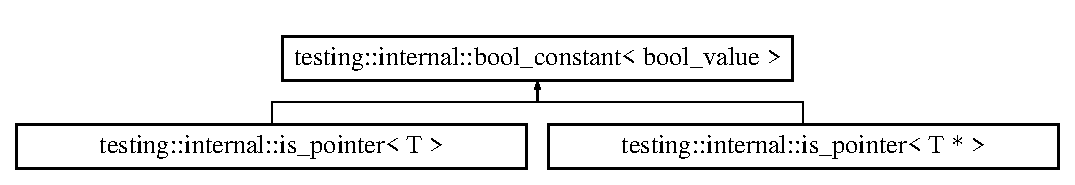
\includegraphics[height=2.000000cm]{structtesting_1_1internal_1_1bool__constant}
\end{center}
\end{figure}
\subsection*{Tipos Públicos}
\begin{DoxyCompactItemize}
\item 
\hypertarget{structtesting_1_1internal_1_1bool__constant_aba6d09ecf7eecea6c93480f0d627a167}{typedef \hyperlink{structtesting_1_1internal_1_1bool__constant}{bool\-\_\-constant}$<$ bool\-\_\-value $>$ {\bfseries type}}\label{structtesting_1_1internal_1_1bool__constant_aba6d09ecf7eecea6c93480f0d627a167}

\end{DoxyCompactItemize}
\subsection*{Atributos Públicos Estáticos}
\begin{DoxyCompactItemize}
\item 
\hypertarget{structtesting_1_1internal_1_1bool__constant_a499fba6576296b04d99690a486424b32}{static const bool {\bfseries value} = bool\-\_\-value}\label{structtesting_1_1internal_1_1bool__constant_a499fba6576296b04d99690a486424b32}

\end{DoxyCompactItemize}


A documentação para esta estrutura foi gerada a partir do seguinte ficheiro\-:\begin{DoxyCompactItemize}
\item 
include/gtest/internal/gtest-\/port.\-h\end{DoxyCompactItemize}

\hypertarget{structstd_1_1tr1_1_1gtest__internal_1_1ByRef}{\section{Referência à estrutura Template std\-:\-:tr1\-:\-:gtest\-\_\-internal\-:\-:By\-Ref$<$ T $>$}
\label{structstd_1_1tr1_1_1gtest__internal_1_1ByRef}\index{std\-::tr1\-::gtest\-\_\-internal\-::\-By\-Ref$<$ T $>$@{std\-::tr1\-::gtest\-\_\-internal\-::\-By\-Ref$<$ T $>$}}
}
\subsection*{Tipos Públicos}
\begin{DoxyCompactItemize}
\item 
\hypertarget{structstd_1_1tr1_1_1gtest__internal_1_1ByRef_ac42ad942ee1cfa86b2abcce9b88ac10e}{typedef const T \& {\bfseries type}}\label{structstd_1_1tr1_1_1gtest__internal_1_1ByRef_ac42ad942ee1cfa86b2abcce9b88ac10e}

\end{DoxyCompactItemize}


A documentação para esta estrutura foi gerada a partir do seguinte ficheiro\-:\begin{DoxyCompactItemize}
\item 
include/gtest/internal/gtest-\/tuple.\-h\end{DoxyCompactItemize}

\hypertarget{structstd_1_1tr1_1_1gtest__internal_1_1ByRef_3_01T_01_6_01_4}{\section{Referência à estrutura Template std\-:\-:tr1\-:\-:gtest\-\_\-internal\-:\-:By\-Ref$<$ T \& $>$}
\label{structstd_1_1tr1_1_1gtest__internal_1_1ByRef_3_01T_01_6_01_4}\index{std\-::tr1\-::gtest\-\_\-internal\-::\-By\-Ref$<$ T \& $>$@{std\-::tr1\-::gtest\-\_\-internal\-::\-By\-Ref$<$ T \& $>$}}
}
\subsection*{Tipos Públicos}
\begin{DoxyCompactItemize}
\item 
\hypertarget{structstd_1_1tr1_1_1gtest__internal_1_1ByRef_3_01T_01_6_01_4_a512382574dbdd736320d68e313801122}{typedef T \& {\bfseries type}}\label{structstd_1_1tr1_1_1gtest__internal_1_1ByRef_3_01T_01_6_01_4_a512382574dbdd736320d68e313801122}

\end{DoxyCompactItemize}


A documentação para esta estrutura foi gerada a partir do seguinte ficheiro\-:\begin{DoxyCompactItemize}
\item 
include/gtest/internal/gtest-\/tuple.\-h\end{DoxyCompactItemize}

\hypertarget{structtesting_1_1internal_1_1CompileAssert}{\section{Referência à estrutura Template testing\-:\-:internal\-:\-:Compile\-Assert$<$ bool $>$}
\label{structtesting_1_1internal_1_1CompileAssert}\index{testing\-::internal\-::\-Compile\-Assert$<$ bool $>$@{testing\-::internal\-::\-Compile\-Assert$<$ bool $>$}}
}


A documentação para esta estrutura foi gerada a partir do seguinte ficheiro\-:\begin{DoxyCompactItemize}
\item 
include/gtest/internal/gtest-\/port.\-h\end{DoxyCompactItemize}

\hypertarget{structtesting_1_1internal_1_1CompileAssertTypesEqual}{\section{Referência à estrutura Template testing\-:\-:internal\-:\-:Compile\-Assert\-Types\-Equal$<$ T1, T2 $>$}
\label{structtesting_1_1internal_1_1CompileAssertTypesEqual}\index{testing\-::internal\-::\-Compile\-Assert\-Types\-Equal$<$ T1, T2 $>$@{testing\-::internal\-::\-Compile\-Assert\-Types\-Equal$<$ T1, T2 $>$}}
}


A documentação para esta estrutura foi gerada a partir do seguinte ficheiro\-:\begin{DoxyCompactItemize}
\item 
include/gtest/internal/gtest-\/internal.\-h\end{DoxyCompactItemize}

\hypertarget{structtesting_1_1internal_1_1CompileAssertTypesEqual_3_01T_00_01T_01_4}{\section{Referência à estrutura Template testing\-:\-:internal\-:\-:Compile\-Assert\-Types\-Equal$<$ T, T $>$}
\label{structtesting_1_1internal_1_1CompileAssertTypesEqual_3_01T_00_01T_01_4}\index{testing\-::internal\-::\-Compile\-Assert\-Types\-Equal$<$ T, T $>$@{testing\-::internal\-::\-Compile\-Assert\-Types\-Equal$<$ T, T $>$}}
}


A documentação para esta estrutura foi gerada a partir do seguinte ficheiro\-:\begin{DoxyCompactItemize}
\item 
include/gtest/internal/gtest-\/internal.\-h\end{DoxyCompactItemize}

\hypertarget{structtesting_1_1internal_1_1ConstCharPtr}{\section{Referência à estrutura testing\-:\-:internal\-:\-:Const\-Char\-Ptr}
\label{structtesting_1_1internal_1_1ConstCharPtr}\index{testing\-::internal\-::\-Const\-Char\-Ptr@{testing\-::internal\-::\-Const\-Char\-Ptr}}
}
\subsection*{Membros públicos}
\begin{DoxyCompactItemize}
\item 
\hypertarget{structtesting_1_1internal_1_1ConstCharPtr_ae94f6453fa679d815994eccc63062907}{{\bfseries Const\-Char\-Ptr} (const char $\ast$str)}\label{structtesting_1_1internal_1_1ConstCharPtr_ae94f6453fa679d815994eccc63062907}

\item 
\hypertarget{structtesting_1_1internal_1_1ConstCharPtr_a891bc286350b81d1a147101c0bae5b1d}{{\bfseries operator bool} () const }\label{structtesting_1_1internal_1_1ConstCharPtr_a891bc286350b81d1a147101c0bae5b1d}

\end{DoxyCompactItemize}
\subsection*{Atributos Públicos}
\begin{DoxyCompactItemize}
\item 
\hypertarget{structtesting_1_1internal_1_1ConstCharPtr_adba40d23d5986904b605946f643cf26e}{const char $\ast$ {\bfseries value}}\label{structtesting_1_1internal_1_1ConstCharPtr_adba40d23d5986904b605946f643cf26e}

\end{DoxyCompactItemize}


A documentação para esta estrutura foi gerada a partir do seguinte ficheiro\-:\begin{DoxyCompactItemize}
\item 
include/gtest/internal/gtest-\/internal.\-h\end{DoxyCompactItemize}

\hypertarget{classtesting_1_1internal_1_1DefaultGlobalTestPartResultReporter}{\section{Referência à classe testing\-:\-:internal\-:\-:Default\-Global\-Test\-Part\-Result\-Reporter}
\label{classtesting_1_1internal_1_1DefaultGlobalTestPartResultReporter}\index{testing\-::internal\-::\-Default\-Global\-Test\-Part\-Result\-Reporter@{testing\-::internal\-::\-Default\-Global\-Test\-Part\-Result\-Reporter}}
}
Diagrama de heranças da classe testing\-:\-:internal\-:\-:Default\-Global\-Test\-Part\-Result\-Reporter\begin{figure}[H]
\begin{center}
\leavevmode
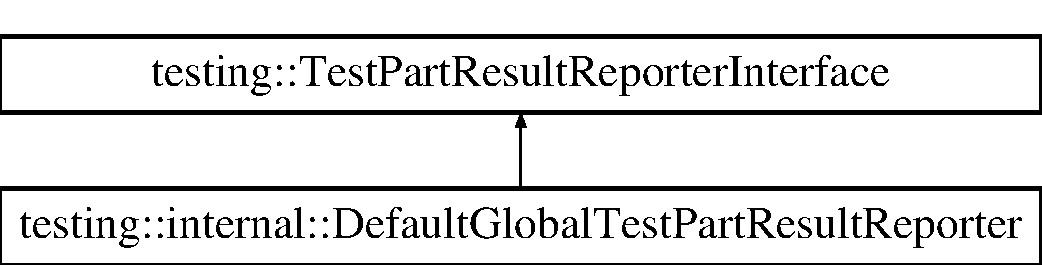
\includegraphics[height=2.000000cm]{classtesting_1_1internal_1_1DefaultGlobalTestPartResultReporter}
\end{center}
\end{figure}
\subsection*{Membros públicos}
\begin{DoxyCompactItemize}
\item 
\hypertarget{classtesting_1_1internal_1_1DefaultGlobalTestPartResultReporter_a3900ea7f34b34afd48c7d1d0312a1488}{{\bfseries Default\-Global\-Test\-Part\-Result\-Reporter} (\hyperlink{classtesting_1_1internal_1_1UnitTestImpl}{Unit\-Test\-Impl} $\ast$unit\-\_\-test)}\label{classtesting_1_1internal_1_1DefaultGlobalTestPartResultReporter_a3900ea7f34b34afd48c7d1d0312a1488}

\item 
\hypertarget{classtesting_1_1internal_1_1DefaultGlobalTestPartResultReporter_a6081576a23b964cfecab1e424d8044fc}{virtual void {\bfseries Report\-Test\-Part\-Result} (const Test\-Part\-Result \&result)}\label{classtesting_1_1internal_1_1DefaultGlobalTestPartResultReporter_a6081576a23b964cfecab1e424d8044fc}

\end{DoxyCompactItemize}


A documentação para esta classe foi gerada a partir dos seguintes ficheiros\-:\begin{DoxyCompactItemize}
\item 
src/gtest-\/internal-\/inl.\-h\item 
src/gtest.\-cc\end{DoxyCompactItemize}

\hypertarget{classtesting_1_1internal_1_1DefaultPerThreadTestPartResultReporter}{\section{Referência à classe testing\-:\-:internal\-:\-:Default\-Per\-Thread\-Test\-Part\-Result\-Reporter}
\label{classtesting_1_1internal_1_1DefaultPerThreadTestPartResultReporter}\index{testing\-::internal\-::\-Default\-Per\-Thread\-Test\-Part\-Result\-Reporter@{testing\-::internal\-::\-Default\-Per\-Thread\-Test\-Part\-Result\-Reporter}}
}
Diagrama de heranças da classe testing\-:\-:internal\-:\-:Default\-Per\-Thread\-Test\-Part\-Result\-Reporter\begin{figure}[H]
\begin{center}
\leavevmode
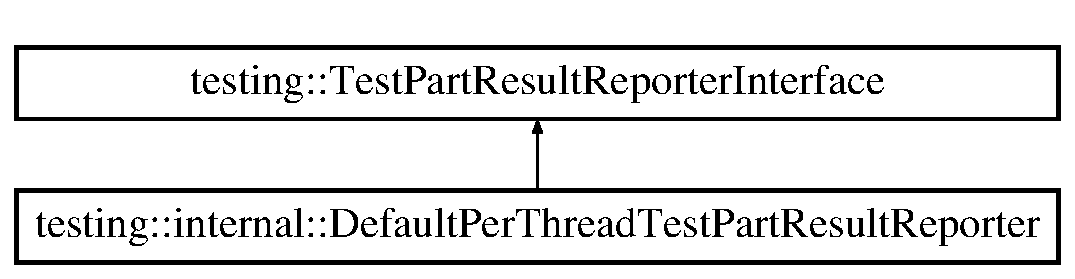
\includegraphics[height=2.000000cm]{classtesting_1_1internal_1_1DefaultPerThreadTestPartResultReporter}
\end{center}
\end{figure}
\subsection*{Membros públicos}
\begin{DoxyCompactItemize}
\item 
\hypertarget{classtesting_1_1internal_1_1DefaultPerThreadTestPartResultReporter_a968a846e5a90d2ffea8b2ce2746099bd}{{\bfseries Default\-Per\-Thread\-Test\-Part\-Result\-Reporter} (\hyperlink{classtesting_1_1internal_1_1UnitTestImpl}{Unit\-Test\-Impl} $\ast$unit\-\_\-test)}\label{classtesting_1_1internal_1_1DefaultPerThreadTestPartResultReporter_a968a846e5a90d2ffea8b2ce2746099bd}

\item 
\hypertarget{classtesting_1_1internal_1_1DefaultPerThreadTestPartResultReporter_ac6dc08eadc4e5a2a64a91d0b6c6b3aad}{virtual void {\bfseries Report\-Test\-Part\-Result} (const \hyperlink{classtesting_1_1TestPartResult}{Test\-Part\-Result} \&result)}\label{classtesting_1_1internal_1_1DefaultPerThreadTestPartResultReporter_ac6dc08eadc4e5a2a64a91d0b6c6b3aad}

\end{DoxyCompactItemize}


A documentação para esta classe foi gerada a partir dos seguintes ficheiros\-:\begin{DoxyCompactItemize}
\item 
src/gtest-\/internal-\/inl.\-h\item 
src/gtest.\-cc\end{DoxyCompactItemize}

\hypertarget{classtesting_1_1EmptyTestEventListener}{\section{Referência à classe testing\-:\-:Empty\-Test\-Event\-Listener}
\label{classtesting_1_1EmptyTestEventListener}\index{testing\-::\-Empty\-Test\-Event\-Listener@{testing\-::\-Empty\-Test\-Event\-Listener}}
}
Diagrama de heranças da classe testing\-:\-:Empty\-Test\-Event\-Listener\begin{figure}[H]
\begin{center}
\leavevmode
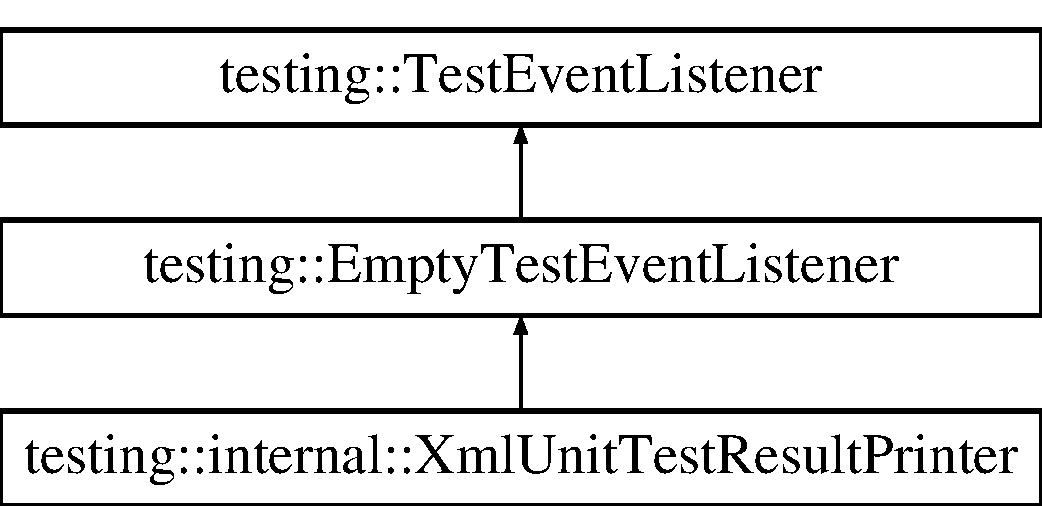
\includegraphics[height=3.000000cm]{classtesting_1_1EmptyTestEventListener}
\end{center}
\end{figure}
\subsection*{Membros públicos}
\begin{DoxyCompactItemize}
\item 
\hypertarget{classtesting_1_1EmptyTestEventListener_aa3847c8a3c22d8d69a6006dfdd6589fc}{virtual void {\bfseries On\-Test\-Program\-Start} (const \hyperlink{classtesting_1_1UnitTest}{Unit\-Test} \&)}\label{classtesting_1_1EmptyTestEventListener_aa3847c8a3c22d8d69a6006dfdd6589fc}

\item 
\hypertarget{classtesting_1_1EmptyTestEventListener_a836f05829855dc60d13ba99ad712c0dd}{virtual void {\bfseries On\-Test\-Iteration\-Start} (const \hyperlink{classtesting_1_1UnitTest}{Unit\-Test} \&, int)}\label{classtesting_1_1EmptyTestEventListener_a836f05829855dc60d13ba99ad712c0dd}

\item 
\hypertarget{classtesting_1_1EmptyTestEventListener_a156d1965248fbdced6aabacadfa2d63f}{virtual void {\bfseries On\-Environments\-Set\-Up\-Start} (const \hyperlink{classtesting_1_1UnitTest}{Unit\-Test} \&)}\label{classtesting_1_1EmptyTestEventListener_a156d1965248fbdced6aabacadfa2d63f}

\item 
\hypertarget{classtesting_1_1EmptyTestEventListener_abc481c6648d15d4242245195a06f5aa0}{virtual void {\bfseries On\-Environments\-Set\-Up\-End} (const \hyperlink{classtesting_1_1UnitTest}{Unit\-Test} \&)}\label{classtesting_1_1EmptyTestEventListener_abc481c6648d15d4242245195a06f5aa0}

\item 
\hypertarget{classtesting_1_1EmptyTestEventListener_ae4707ed9cc7ace5241bc8ccc4051209b}{virtual void {\bfseries On\-Test\-Case\-Start} (const \hyperlink{classtesting_1_1TestCase}{Test\-Case} \&)}\label{classtesting_1_1EmptyTestEventListener_ae4707ed9cc7ace5241bc8ccc4051209b}

\item 
\hypertarget{classtesting_1_1EmptyTestEventListener_a84fa74cc9ba742f9f847ea405ca84e5e}{virtual void {\bfseries On\-Test\-Start} (const \hyperlink{classtesting_1_1TestInfo}{Test\-Info} \&)}\label{classtesting_1_1EmptyTestEventListener_a84fa74cc9ba742f9f847ea405ca84e5e}

\item 
\hypertarget{classtesting_1_1EmptyTestEventListener_a59e7f7d9f2e2d089a6e8c1e2577f4718}{virtual void {\bfseries On\-Test\-Part\-Result} (const \hyperlink{classtesting_1_1TestPartResult}{Test\-Part\-Result} \&)}\label{classtesting_1_1EmptyTestEventListener_a59e7f7d9f2e2d089a6e8c1e2577f4718}

\item 
\hypertarget{classtesting_1_1EmptyTestEventListener_afd58d21005f0d0d0399fb114627545d3}{virtual void {\bfseries On\-Test\-End} (const \hyperlink{classtesting_1_1TestInfo}{Test\-Info} \&)}\label{classtesting_1_1EmptyTestEventListener_afd58d21005f0d0d0399fb114627545d3}

\item 
\hypertarget{classtesting_1_1EmptyTestEventListener_a6bec703158283104c4298f7d8a528515}{virtual void {\bfseries On\-Test\-Case\-End} (const \hyperlink{classtesting_1_1TestCase}{Test\-Case} \&)}\label{classtesting_1_1EmptyTestEventListener_a6bec703158283104c4298f7d8a528515}

\item 
\hypertarget{classtesting_1_1EmptyTestEventListener_a00fa1a4ea5831e20746188414268e7c6}{virtual void {\bfseries On\-Environments\-Tear\-Down\-Start} (const \hyperlink{classtesting_1_1UnitTest}{Unit\-Test} \&)}\label{classtesting_1_1EmptyTestEventListener_a00fa1a4ea5831e20746188414268e7c6}

\item 
\hypertarget{classtesting_1_1EmptyTestEventListener_aea64c83c415b33a4c0b0239bafd1438d}{virtual void {\bfseries On\-Environments\-Tear\-Down\-End} (const \hyperlink{classtesting_1_1UnitTest}{Unit\-Test} \&)}\label{classtesting_1_1EmptyTestEventListener_aea64c83c415b33a4c0b0239bafd1438d}

\item 
\hypertarget{classtesting_1_1EmptyTestEventListener_a2253e5a18b3cf7bccd349567a252209d}{virtual void {\bfseries On\-Test\-Iteration\-End} (const \hyperlink{classtesting_1_1UnitTest}{Unit\-Test} \&, int)}\label{classtesting_1_1EmptyTestEventListener_a2253e5a18b3cf7bccd349567a252209d}

\item 
\hypertarget{classtesting_1_1EmptyTestEventListener_a0abcc02bd2331a2e29ad6f4d9daf2a32}{virtual void {\bfseries On\-Test\-Program\-End} (const \hyperlink{classtesting_1_1UnitTest}{Unit\-Test} \&)}\label{classtesting_1_1EmptyTestEventListener_a0abcc02bd2331a2e29ad6f4d9daf2a32}

\end{DoxyCompactItemize}


A documentação para esta classe foi gerada a partir do seguinte ficheiro\-:\begin{DoxyCompactItemize}
\item 
include/gtest/gtest.\-h\end{DoxyCompactItemize}

\hypertarget{structtesting_1_1internal_1_1EnableIf}{\section{Referência à estrutura Template testing\-:\-:internal\-:\-:Enable\-If$<$ bool $>$}
\label{structtesting_1_1internal_1_1EnableIf}\index{testing\-::internal\-::\-Enable\-If$<$ bool $>$@{testing\-::internal\-::\-Enable\-If$<$ bool $>$}}
}


A documentação para esta estrutura foi gerada a partir do seguinte ficheiro\-:\begin{DoxyCompactItemize}
\item 
include/gtest/internal/gtest-\/internal.\-h\end{DoxyCompactItemize}

\hypertarget{structtesting_1_1internal_1_1EnableIf_3_01true_01_4}{\section{Referência à estrutura Template testing\-:\-:internal\-:\-:Enable\-If$<$ true $>$}
\label{structtesting_1_1internal_1_1EnableIf_3_01true_01_4}\index{testing\-::internal\-::\-Enable\-If$<$ true $>$@{testing\-::internal\-::\-Enable\-If$<$ true $>$}}
}
\subsection*{Tipos Públicos}
\begin{DoxyCompactItemize}
\item 
\hypertarget{structtesting_1_1internal_1_1EnableIf_3_01true_01_4_a9398d803f1fdd99ff41823746f6299ff}{typedef void {\bfseries type}}\label{structtesting_1_1internal_1_1EnableIf_3_01true_01_4_a9398d803f1fdd99ff41823746f6299ff}

\end{DoxyCompactItemize}


A documentação para esta estrutura foi gerada a partir do seguinte ficheiro\-:\begin{DoxyCompactItemize}
\item 
include/gtest/internal/gtest-\/internal.\-h\end{DoxyCompactItemize}

\hypertarget{classtesting_1_1Environment}{\section{Referência à classe testing\-:\-:Environment}
\label{classtesting_1_1Environment}\index{testing\-::\-Environment@{testing\-::\-Environment}}
}
\subsection*{Membros públicos}
\begin{DoxyCompactItemize}
\item 
\hypertarget{classtesting_1_1Environment_a1bf8cafaa9d4eba9feb98655ee434eb3}{virtual void {\bfseries Set\-Up} ()}\label{classtesting_1_1Environment_a1bf8cafaa9d4eba9feb98655ee434eb3}

\item 
\hypertarget{classtesting_1_1Environment_a039bdaa705c46b9b88234cf4d3bb6254}{virtual void {\bfseries Tear\-Down} ()}\label{classtesting_1_1Environment_a039bdaa705c46b9b88234cf4d3bb6254}

\end{DoxyCompactItemize}


A documentação para esta classe foi gerada a partir do seguinte ficheiro\-:\begin{DoxyCompactItemize}
\item 
include/gtest/gtest.\-h\end{DoxyCompactItemize}

\hypertarget{classtesting_1_1internal_1_1EqHelper}{\section{Referência à classe Template testing\-:\-:internal\-:\-:Eq\-Helper$<$ lhs\-\_\-is\-\_\-null\-\_\-literal $>$}
\label{classtesting_1_1internal_1_1EqHelper}\index{testing\-::internal\-::\-Eq\-Helper$<$ lhs\-\_\-is\-\_\-null\-\_\-literal $>$@{testing\-::internal\-::\-Eq\-Helper$<$ lhs\-\_\-is\-\_\-null\-\_\-literal $>$}}
}
\subsection*{Membros públicos estáticos}
\begin{DoxyCompactItemize}
\item 
\hypertarget{classtesting_1_1internal_1_1EqHelper_ac2977ed90cd3c88607f804e43b86b92c}{{\footnotesize template$<$typename T1 , typename T2 $>$ }\\static \hyperlink{classtesting_1_1AssertionResult}{Assertion\-Result} {\bfseries Compare} (const char $\ast$expected\-\_\-expression, const char $\ast$actual\-\_\-expression, const T1 \&expected, const T2 \&actual)}\label{classtesting_1_1internal_1_1EqHelper_ac2977ed90cd3c88607f804e43b86b92c}

\item 
\hypertarget{classtesting_1_1internal_1_1EqHelper_a3de996954b41d484c065ed824fe7eac9}{static \hyperlink{classtesting_1_1AssertionResult}{Assertion\-Result} {\bfseries Compare} (const char $\ast$expected\-\_\-expression, const char $\ast$actual\-\_\-expression, Biggest\-Int expected, Biggest\-Int actual)}\label{classtesting_1_1internal_1_1EqHelper_a3de996954b41d484c065ed824fe7eac9}

\end{DoxyCompactItemize}


A documentação para esta classe foi gerada a partir do seguinte ficheiro\-:\begin{DoxyCompactItemize}
\item 
include/gtest/gtest.\-h\end{DoxyCompactItemize}

\hypertarget{classtesting_1_1internal_1_1EqHelper_3_01true_01_4}{\section{Referência à classe Template testing\-:\-:internal\-:\-:Eq\-Helper$<$ true $>$}
\label{classtesting_1_1internal_1_1EqHelper_3_01true_01_4}\index{testing\-::internal\-::\-Eq\-Helper$<$ true $>$@{testing\-::internal\-::\-Eq\-Helper$<$ true $>$}}
}
\subsection*{Membros públicos estáticos}
\begin{DoxyCompactItemize}
\item 
\hypertarget{classtesting_1_1internal_1_1EqHelper_3_01true_01_4_a70d6d7e3cb1df06ad6114f25e843fd6d}{{\footnotesize template$<$typename T1 , typename T2 $>$ }\\static \hyperlink{classtesting_1_1AssertionResult}{Assertion\-Result} {\bfseries Compare} (const char $\ast$expected\-\_\-expression, const char $\ast$actual\-\_\-expression, const T1 \&expected, const T2 \&actual, typename \hyperlink{structtesting_1_1internal_1_1EnableIf}{Enable\-If}$<$!\hyperlink{structtesting_1_1internal_1_1is__pointer}{is\-\_\-pointer}$<$ T2 $>$\-::value $>$\-::type $\ast$=0)}\label{classtesting_1_1internal_1_1EqHelper_3_01true_01_4_a70d6d7e3cb1df06ad6114f25e843fd6d}

\item 
\hypertarget{classtesting_1_1internal_1_1EqHelper_3_01true_01_4_ab38e840297adb48f18767a1a99187fb3}{{\footnotesize template$<$typename T $>$ }\\static \hyperlink{classtesting_1_1AssertionResult}{Assertion\-Result} {\bfseries Compare} (const char $\ast$expected\-\_\-expression, const char $\ast$actual\-\_\-expression, Secret $\ast$, T $\ast$actual)}\label{classtesting_1_1internal_1_1EqHelper_3_01true_01_4_ab38e840297adb48f18767a1a99187fb3}

\end{DoxyCompactItemize}


A documentação para esta classe foi gerada a partir do seguinte ficheiro\-:\begin{DoxyCompactItemize}
\item 
include/gtest/gtest.\-h\end{DoxyCompactItemize}

\hypertarget{classtesting_1_1internal_1_1FilePath}{\section{Referência à classe testing\-:\-:internal\-:\-:File\-Path}
\label{classtesting_1_1internal_1_1FilePath}\index{testing\-::internal\-::\-File\-Path@{testing\-::internal\-::\-File\-Path}}
}
\subsection*{Membros públicos}
\begin{DoxyCompactItemize}
\item 
\hypertarget{classtesting_1_1internal_1_1FilePath_ae9efd0fee56c6e3e2d659b464250b112}{{\bfseries File\-Path} (const \hyperlink{classtesting_1_1internal_1_1FilePath}{File\-Path} \&rhs)}\label{classtesting_1_1internal_1_1FilePath_ae9efd0fee56c6e3e2d659b464250b112}

\item 
\hypertarget{classtesting_1_1internal_1_1FilePath_a9fc072b140aa0652a7022fb809fe3abe}{{\bfseries File\-Path} (const std\-::string \&pathname)}\label{classtesting_1_1internal_1_1FilePath_a9fc072b140aa0652a7022fb809fe3abe}

\item 
\hypertarget{classtesting_1_1internal_1_1FilePath_a8d9c1bafb90f10bcd5611a54d8f326ef}{\hyperlink{classtesting_1_1internal_1_1FilePath}{File\-Path} \& {\bfseries operator=} (const \hyperlink{classtesting_1_1internal_1_1FilePath}{File\-Path} \&rhs)}\label{classtesting_1_1internal_1_1FilePath_a8d9c1bafb90f10bcd5611a54d8f326ef}

\item 
\hypertarget{classtesting_1_1internal_1_1FilePath_a15a42de7518e89254e0640dd9317d5f7}{void {\bfseries Set} (const \hyperlink{classtesting_1_1internal_1_1FilePath}{File\-Path} \&rhs)}\label{classtesting_1_1internal_1_1FilePath_a15a42de7518e89254e0640dd9317d5f7}

\item 
\hypertarget{classtesting_1_1internal_1_1FilePath_a7c544a30af67e2da5ce7e625f8402818}{const std\-::string \& {\bfseries string} () const }\label{classtesting_1_1internal_1_1FilePath_a7c544a30af67e2da5ce7e625f8402818}

\item 
\hypertarget{classtesting_1_1internal_1_1FilePath_a85297234dac0acd936632dff8634c2b9}{const char $\ast$ {\bfseries c\-\_\-str} () const }\label{classtesting_1_1internal_1_1FilePath_a85297234dac0acd936632dff8634c2b9}

\item 
\hypertarget{classtesting_1_1internal_1_1FilePath_a44543ff34ae757038ab20925659b447a}{bool {\bfseries Is\-Empty} () const }\label{classtesting_1_1internal_1_1FilePath_a44543ff34ae757038ab20925659b447a}

\item 
\hypertarget{classtesting_1_1internal_1_1FilePath_a952e1b2a9909cdeaf25de5fcdf069b3a}{\hyperlink{classtesting_1_1internal_1_1FilePath}{File\-Path} {\bfseries Remove\-Trailing\-Path\-Separator} () const }\label{classtesting_1_1internal_1_1FilePath_a952e1b2a9909cdeaf25de5fcdf069b3a}

\item 
\hypertarget{classtesting_1_1internal_1_1FilePath_a2852e5a759ff2e2620c7317b8121d757}{\hyperlink{classtesting_1_1internal_1_1FilePath}{File\-Path} {\bfseries Remove\-Directory\-Name} () const }\label{classtesting_1_1internal_1_1FilePath_a2852e5a759ff2e2620c7317b8121d757}

\item 
\hypertarget{classtesting_1_1internal_1_1FilePath_aed3abcd0b8a7f6ed1ff0e7743ef8bf1e}{\hyperlink{classtesting_1_1internal_1_1FilePath}{File\-Path} {\bfseries Remove\-File\-Name} () const }\label{classtesting_1_1internal_1_1FilePath_aed3abcd0b8a7f6ed1ff0e7743ef8bf1e}

\item 
\hypertarget{classtesting_1_1internal_1_1FilePath_ab2a25cc916c111597b94d006aa973c3d}{\hyperlink{classtesting_1_1internal_1_1FilePath}{File\-Path} {\bfseries Remove\-Extension} (const char $\ast$extension) const }\label{classtesting_1_1internal_1_1FilePath_ab2a25cc916c111597b94d006aa973c3d}

\item 
\hypertarget{classtesting_1_1internal_1_1FilePath_afccf35a45e209c22e68c6f8e86036c12}{bool {\bfseries Create\-Directories\-Recursively} () const }\label{classtesting_1_1internal_1_1FilePath_afccf35a45e209c22e68c6f8e86036c12}

\item 
\hypertarget{classtesting_1_1internal_1_1FilePath_a303cdda61bee6e8a0b0303e8fc857e36}{bool {\bfseries Create\-Folder} () const }\label{classtesting_1_1internal_1_1FilePath_a303cdda61bee6e8a0b0303e8fc857e36}

\item 
\hypertarget{classtesting_1_1internal_1_1FilePath_a3548d3ead0e94701669afc64d765ece7}{bool {\bfseries File\-Or\-Directory\-Exists} () const }\label{classtesting_1_1internal_1_1FilePath_a3548d3ead0e94701669afc64d765ece7}

\item 
\hypertarget{classtesting_1_1internal_1_1FilePath_a3546b3f926935fefddb9a808e7e2be47}{bool {\bfseries Directory\-Exists} () const }\label{classtesting_1_1internal_1_1FilePath_a3546b3f926935fefddb9a808e7e2be47}

\item 
\hypertarget{classtesting_1_1internal_1_1FilePath_a918336f16efa8e07d4b94192d6a89f44}{bool {\bfseries Is\-Directory} () const }\label{classtesting_1_1internal_1_1FilePath_a918336f16efa8e07d4b94192d6a89f44}

\item 
\hypertarget{classtesting_1_1internal_1_1FilePath_a7d31c82f3f979c54e5a985382b52feb1}{bool {\bfseries Is\-Root\-Directory} () const }\label{classtesting_1_1internal_1_1FilePath_a7d31c82f3f979c54e5a985382b52feb1}

\item 
\hypertarget{classtesting_1_1internal_1_1FilePath_a720a5f0fd00f3e98d6f3518f4dadfff5}{bool {\bfseries Is\-Absolute\-Path} () const }\label{classtesting_1_1internal_1_1FilePath_a720a5f0fd00f3e98d6f3518f4dadfff5}

\end{DoxyCompactItemize}
\subsection*{Membros públicos estáticos}
\begin{DoxyCompactItemize}
\item 
\hypertarget{classtesting_1_1internal_1_1FilePath_aaff39ccd7bfb7a1c09c0220a64326387}{static \hyperlink{classtesting_1_1internal_1_1FilePath}{File\-Path} {\bfseries Get\-Current\-Dir} ()}\label{classtesting_1_1internal_1_1FilePath_aaff39ccd7bfb7a1c09c0220a64326387}

\item 
\hypertarget{classtesting_1_1internal_1_1FilePath_aa8c102da670261eb4fa8e2f2481df139}{static \hyperlink{classtesting_1_1internal_1_1FilePath}{File\-Path} {\bfseries Make\-File\-Name} (const \hyperlink{classtesting_1_1internal_1_1FilePath}{File\-Path} \&directory, const \hyperlink{classtesting_1_1internal_1_1FilePath}{File\-Path} \&base\-\_\-name, int number, const char $\ast$extension)}\label{classtesting_1_1internal_1_1FilePath_aa8c102da670261eb4fa8e2f2481df139}

\item 
\hypertarget{classtesting_1_1internal_1_1FilePath_ac9d57987f60ac43f0c57b89e333e531e}{static \hyperlink{classtesting_1_1internal_1_1FilePath}{File\-Path} {\bfseries Concat\-Paths} (const \hyperlink{classtesting_1_1internal_1_1FilePath}{File\-Path} \&directory, const \hyperlink{classtesting_1_1internal_1_1FilePath}{File\-Path} \&relative\-\_\-path)}\label{classtesting_1_1internal_1_1FilePath_ac9d57987f60ac43f0c57b89e333e531e}

\item 
\hypertarget{classtesting_1_1internal_1_1FilePath_a2280a77adb394cf80bb5f73fc292e8c8}{static \hyperlink{classtesting_1_1internal_1_1FilePath}{File\-Path} {\bfseries Generate\-Unique\-File\-Name} (const \hyperlink{classtesting_1_1internal_1_1FilePath}{File\-Path} \&directory, const \hyperlink{classtesting_1_1internal_1_1FilePath}{File\-Path} \&base\-\_\-name, const char $\ast$extension)}\label{classtesting_1_1internal_1_1FilePath_a2280a77adb394cf80bb5f73fc292e8c8}

\end{DoxyCompactItemize}


A documentação para esta classe foi gerada a partir dos seguintes ficheiros\-:\begin{DoxyCompactItemize}
\item 
include/gtest/internal/gtest-\/filepath.\-h\item 
src/gtest-\/filepath.\-cc\end{DoxyCompactItemize}

\hypertarget{classtesting_1_1internal_1_1FloatingPoint}{\section{Referência à classe Template testing\-:\-:internal\-:\-:Floating\-Point$<$ Raw\-Type $>$}
\label{classtesting_1_1internal_1_1FloatingPoint}\index{testing\-::internal\-::\-Floating\-Point$<$ Raw\-Type $>$@{testing\-::internal\-::\-Floating\-Point$<$ Raw\-Type $>$}}
}
\subsection*{Tipos Públicos}
\begin{DoxyCompactItemize}
\item 
\hypertarget{classtesting_1_1internal_1_1FloatingPoint_abf228bf6cd48f12c8b44c85b4971a731}{typedef \hyperlink{classtesting_1_1internal_1_1TypeWithSize}{Type\-With\-Size}$<$ sizeof(Raw\-Type)$>$\\*
\-::U\-Int {\bfseries Bits}}\label{classtesting_1_1internal_1_1FloatingPoint_abf228bf6cd48f12c8b44c85b4971a731}

\end{DoxyCompactItemize}
\subsection*{Membros públicos}
\begin{DoxyCompactItemize}
\item 
\hypertarget{classtesting_1_1internal_1_1FloatingPoint_a0dabf840863e0df84046f171c891fe71}{{\bfseries Floating\-Point} (const Raw\-Type \&x)}\label{classtesting_1_1internal_1_1FloatingPoint_a0dabf840863e0df84046f171c891fe71}

\item 
\hypertarget{classtesting_1_1internal_1_1FloatingPoint_abead51f16ec6ea84360a976da1cd1387}{const Bits \& {\bfseries bits} () const }\label{classtesting_1_1internal_1_1FloatingPoint_abead51f16ec6ea84360a976da1cd1387}

\item 
\hypertarget{classtesting_1_1internal_1_1FloatingPoint_af53c50b85408c582540d6244c026ce2b}{Bits {\bfseries exponent\-\_\-bits} () const }\label{classtesting_1_1internal_1_1FloatingPoint_af53c50b85408c582540d6244c026ce2b}

\item 
\hypertarget{classtesting_1_1internal_1_1FloatingPoint_aa0167b7b10a934b743ba3c1f47421e63}{Bits {\bfseries fraction\-\_\-bits} () const }\label{classtesting_1_1internal_1_1FloatingPoint_aa0167b7b10a934b743ba3c1f47421e63}

\item 
\hypertarget{classtesting_1_1internal_1_1FloatingPoint_a6176cc4d443724477f2799bcbd9f020a}{Bits {\bfseries sign\-\_\-bit} () const }\label{classtesting_1_1internal_1_1FloatingPoint_a6176cc4d443724477f2799bcbd9f020a}

\item 
\hypertarget{classtesting_1_1internal_1_1FloatingPoint_aaef2fd2cd8cdf791206a5e9fed8ef90d}{bool {\bfseries is\-\_\-nan} () const }\label{classtesting_1_1internal_1_1FloatingPoint_aaef2fd2cd8cdf791206a5e9fed8ef90d}

\item 
\hypertarget{classtesting_1_1internal_1_1FloatingPoint_adb0fe9ab1d9e5288f8e5550234211166}{bool {\bfseries Almost\-Equals} (const \hyperlink{classtesting_1_1internal_1_1FloatingPoint}{Floating\-Point} \&rhs) const }\label{classtesting_1_1internal_1_1FloatingPoint_adb0fe9ab1d9e5288f8e5550234211166}

\item 
\hypertarget{classtesting_1_1internal_1_1FloatingPoint_af2eda9331e679229a1baa3404b57b51d}{{\footnotesize template$<$$>$ }\\float {\bfseries Max} ()}\label{classtesting_1_1internal_1_1FloatingPoint_af2eda9331e679229a1baa3404b57b51d}

\item 
\hypertarget{classtesting_1_1internal_1_1FloatingPoint_afc2e85c0e886cb13b2300e961c9a9648}{{\footnotesize template$<$$>$ }\\double {\bfseries Max} ()}\label{classtesting_1_1internal_1_1FloatingPoint_afc2e85c0e886cb13b2300e961c9a9648}

\end{DoxyCompactItemize}
\subsection*{Membros públicos estáticos}
\begin{DoxyCompactItemize}
\item 
\hypertarget{classtesting_1_1internal_1_1FloatingPoint_ac551f793522e54fbd8a25acb79eac5b1}{static Raw\-Type {\bfseries Reinterpret\-Bits} (const Bits bits)}\label{classtesting_1_1internal_1_1FloatingPoint_ac551f793522e54fbd8a25acb79eac5b1}

\item 
\hypertarget{classtesting_1_1internal_1_1FloatingPoint_a460027cc19cf01ae8e09cc3796b2b575}{static Raw\-Type {\bfseries Infinity} ()}\label{classtesting_1_1internal_1_1FloatingPoint_a460027cc19cf01ae8e09cc3796b2b575}

\item 
\hypertarget{classtesting_1_1internal_1_1FloatingPoint_aae5954d8a57d3ff0987c6930cb68e114}{static Raw\-Type {\bfseries Max} ()}\label{classtesting_1_1internal_1_1FloatingPoint_aae5954d8a57d3ff0987c6930cb68e114}

\end{DoxyCompactItemize}
\subsection*{Atributos Públicos Estáticos}
\begin{DoxyCompactItemize}
\item 
\hypertarget{classtesting_1_1internal_1_1FloatingPoint_ab819d2e8f93e9e482373999f0f8d71b9}{static const size\-\_\-t {\bfseries k\-Bit\-Count} = 8$\ast$sizeof(Raw\-Type)}\label{classtesting_1_1internal_1_1FloatingPoint_ab819d2e8f93e9e482373999f0f8d71b9}

\item 
static const size\-\_\-t {\bfseries k\-Fraction\-Bit\-Count}
\item 
\hypertarget{classtesting_1_1internal_1_1FloatingPoint_a1973d843c00781053d3073daa8a40119}{static const size\-\_\-t {\bfseries k\-Exponent\-Bit\-Count} = k\-Bit\-Count -\/ 1 -\/ k\-Fraction\-Bit\-Count}\label{classtesting_1_1internal_1_1FloatingPoint_a1973d843c00781053d3073daa8a40119}

\item 
\hypertarget{classtesting_1_1internal_1_1FloatingPoint_aca98b5ea6f2222a66a82e52421682efa}{static const Bits {\bfseries k\-Sign\-Bit\-Mask} = static\-\_\-cast$<$Bits$>$(1) $<$$<$ (k\-Bit\-Count -\/ 1)}\label{classtesting_1_1internal_1_1FloatingPoint_aca98b5ea6f2222a66a82e52421682efa}

\item 
static const Bits {\bfseries k\-Fraction\-Bit\-Mask}
\item 
\hypertarget{classtesting_1_1internal_1_1FloatingPoint_a66065dfc4d5f41100f686159637af23b}{static const Bits {\bfseries k\-Exponent\-Bit\-Mask} = $\sim$(k\-Sign\-Bit\-Mask $\vert$ k\-Fraction\-Bit\-Mask)}\label{classtesting_1_1internal_1_1FloatingPoint_a66065dfc4d5f41100f686159637af23b}

\item 
\hypertarget{classtesting_1_1internal_1_1FloatingPoint_aac498b3714d93f8e88cdc30e4c5935f6}{static const size\-\_\-t {\bfseries k\-Max\-Ulps} = 4}\label{classtesting_1_1internal_1_1FloatingPoint_aac498b3714d93f8e88cdc30e4c5935f6}

\end{DoxyCompactItemize}


\subsection{Documentação dos dados membro}
\hypertarget{classtesting_1_1internal_1_1FloatingPoint_a0b756a6d2a4f5f5b41ca79651c06c043}{\index{testing\-::internal\-::\-Floating\-Point@{testing\-::internal\-::\-Floating\-Point}!k\-Fraction\-Bit\-Count@{k\-Fraction\-Bit\-Count}}
\index{k\-Fraction\-Bit\-Count@{k\-Fraction\-Bit\-Count}!testing::internal::FloatingPoint@{testing\-::internal\-::\-Floating\-Point}}
\subsubsection[{k\-Fraction\-Bit\-Count}]{\setlength{\rightskip}{0pt plus 5cm}template$<$typename Raw\-Type $>$ const size\-\_\-t {\bf testing\-::internal\-::\-Floating\-Point}$<$ Raw\-Type $>$\-::k\-Fraction\-Bit\-Count\hspace{0.3cm}{\ttfamily [static]}}}\label{classtesting_1_1internal_1_1FloatingPoint_a0b756a6d2a4f5f5b41ca79651c06c043}
{\bfseries Valor inicial\-:}
\begin{DoxyCode}
=
    std::numeric\_limits<RawType>::digits - 1
\end{DoxyCode}
\hypertarget{classtesting_1_1internal_1_1FloatingPoint_a0ac75d4ffd24f14bca452abe8a718da1}{\index{testing\-::internal\-::\-Floating\-Point@{testing\-::internal\-::\-Floating\-Point}!k\-Fraction\-Bit\-Mask@{k\-Fraction\-Bit\-Mask}}
\index{k\-Fraction\-Bit\-Mask@{k\-Fraction\-Bit\-Mask}!testing::internal::FloatingPoint@{testing\-::internal\-::\-Floating\-Point}}
\subsubsection[{k\-Fraction\-Bit\-Mask}]{\setlength{\rightskip}{0pt plus 5cm}template$<$typename Raw\-Type $>$ const Bits {\bf testing\-::internal\-::\-Floating\-Point}$<$ Raw\-Type $>$\-::k\-Fraction\-Bit\-Mask\hspace{0.3cm}{\ttfamily [static]}}}\label{classtesting_1_1internal_1_1FloatingPoint_a0ac75d4ffd24f14bca452abe8a718da1}
{\bfseries Valor inicial\-:}
\begin{DoxyCode}
=
    ~static\_cast<Bits>(0) >> (kExponentBitCount + 1)
\end{DoxyCode}


A documentação para esta classe foi gerada a partir do seguinte ficheiro\-:\begin{DoxyCompactItemize}
\item 
include/gtest/internal/gtest-\/internal.\-h\end{DoxyCompactItemize}

\hypertarget{classtesting_1_1internal_1_1FormatForComparison}{\section{Referência à classe Template testing\-:\-:internal\-:\-:Format\-For\-Comparison$<$ To\-Print, Other\-Operand $>$}
\label{classtesting_1_1internal_1_1FormatForComparison}\index{testing\-::internal\-::\-Format\-For\-Comparison$<$ To\-Print, Other\-Operand $>$@{testing\-::internal\-::\-Format\-For\-Comparison$<$ To\-Print, Other\-Operand $>$}}
}
\subsection*{Membros públicos estáticos}
\begin{DoxyCompactItemize}
\item 
\hypertarget{classtesting_1_1internal_1_1FormatForComparison_a2aeb688fc55b57abd3021d82eccad896}{\-::std\-::string {\bfseries Format} (const To\-Print \&value)}\label{classtesting_1_1internal_1_1FormatForComparison_a2aeb688fc55b57abd3021d82eccad896}

\end{DoxyCompactItemize}


A documentação para esta classe foi gerada a partir do seguinte ficheiro\-:\begin{DoxyCompactItemize}
\item 
include/gtest/gtest.\-h\end{DoxyCompactItemize}

\hypertarget{classtesting_1_1internal_1_1FormatForComparison_3_01ToPrint[N]_00_01OtherOperand_01_4}{\section{Referência à classe Template testing\-:\-:internal\-:\-:Format\-For\-Comparison$<$ To\-Print\mbox{[}N\mbox{]}, Other\-Operand $>$}
\label{classtesting_1_1internal_1_1FormatForComparison_3_01ToPrint[N]_00_01OtherOperand_01_4}\index{testing\-::internal\-::\-Format\-For\-Comparison$<$ To\-Print\mbox{[}\-N\mbox{]}, Other\-Operand $>$@{testing\-::internal\-::\-Format\-For\-Comparison$<$ To\-Print[N], Other\-Operand $>$}}
}
\subsection*{Membros públicos estáticos}
\begin{DoxyCompactItemize}
\item 
\hypertarget{classtesting_1_1internal_1_1FormatForComparison_3_01ToPrint[N]_00_01OtherOperand_01_4_a76c526461c8fa7df75f7b32ab889b9e0}{\-::std\-::string {\bfseries Format} (const To\-Print $\ast$value)}\label{classtesting_1_1internal_1_1FormatForComparison_3_01ToPrint[N]_00_01OtherOperand_01_4_a76c526461c8fa7df75f7b32ab889b9e0}

\end{DoxyCompactItemize}


A documentação para esta classe foi gerada a partir do seguinte ficheiro\-:\begin{DoxyCompactItemize}
\item 
include/gtest/gtest.\-h\end{DoxyCompactItemize}

\hypertarget{classstd_1_1tr1_1_1gtest__internal_1_1Get}{\section{Referência à classe Template std\-:\-:tr1\-:\-:gtest\-\_\-internal\-:\-:Get$<$ k $>$}
\label{classstd_1_1tr1_1_1gtest__internal_1_1Get}\index{std\-::tr1\-::gtest\-\_\-internal\-::\-Get$<$ k $>$@{std\-::tr1\-::gtest\-\_\-internal\-::\-Get$<$ k $>$}}
}


A documentação para esta classe foi gerada a partir do seguinte ficheiro\-:\begin{DoxyCompactItemize}
\item 
include/gtest/internal/gtest-\/tuple.\-h\end{DoxyCompactItemize}

\hypertarget{classstd_1_1tr1_1_1gtest__internal_1_1Get_3_010_01_4}{\section{Referência à classe Template std\-:\-:tr1\-:\-:gtest\-\_\-internal\-:\-:Get$<$ 0 $>$}
\label{classstd_1_1tr1_1_1gtest__internal_1_1Get_3_010_01_4}\index{std\-::tr1\-::gtest\-\_\-internal\-::\-Get$<$ 0 $>$@{std\-::tr1\-::gtest\-\_\-internal\-::\-Get$<$ 0 $>$}}
}
\subsection*{Membros públicos estáticos}
\begin{DoxyCompactItemize}
\item 
\hypertarget{classstd_1_1tr1_1_1gtest__internal_1_1Get_3_010_01_4_a74beca3869fddfe42ee608b7f4cacb96}{{\footnotesize template$<$class Tuple $>$ }\\static {\bfseries G\-T\-E\-S\-T\-\_\-\-A\-D\-D\-\_\-\-R\-E\-F\-\_\-} (G\-T\-E\-S\-T\-\_\-\-T\-U\-P\-L\-E\-\_\-\-E\-L\-E\-M\-E\-N\-T\-\_\-(0, Tuple)) Field(Tuple \&t)}\label{classstd_1_1tr1_1_1gtest__internal_1_1Get_3_010_01_4_a74beca3869fddfe42ee608b7f4cacb96}

\item 
\hypertarget{classstd_1_1tr1_1_1gtest__internal_1_1Get_3_010_01_4_a195b3853de45077f9a324c455f22d7e2}{{\footnotesize template$<$class Tuple $>$ }\\static {\bfseries G\-T\-E\-S\-T\-\_\-\-B\-Y\-\_\-\-R\-E\-F\-\_\-} (G\-T\-E\-S\-T\-\_\-\-T\-U\-P\-L\-E\-\_\-\-E\-L\-E\-M\-E\-N\-T\-\_\-(0, Tuple)) Const\-Field(const Tuple \&t)}\label{classstd_1_1tr1_1_1gtest__internal_1_1Get_3_010_01_4_a195b3853de45077f9a324c455f22d7e2}

\end{DoxyCompactItemize}


A documentação para esta classe foi gerada a partir do seguinte ficheiro\-:\begin{DoxyCompactItemize}
\item 
include/gtest/internal/gtest-\/tuple.\-h\end{DoxyCompactItemize}

\hypertarget{classstd_1_1tr1_1_1gtest__internal_1_1Get_3_011_01_4}{\section{Referência à classe Template std\-:\-:tr1\-:\-:gtest\-\_\-internal\-:\-:Get$<$ 1 $>$}
\label{classstd_1_1tr1_1_1gtest__internal_1_1Get_3_011_01_4}\index{std\-::tr1\-::gtest\-\_\-internal\-::\-Get$<$ 1 $>$@{std\-::tr1\-::gtest\-\_\-internal\-::\-Get$<$ 1 $>$}}
}
\subsection*{Membros públicos estáticos}
\begin{DoxyCompactItemize}
\item 
\hypertarget{classstd_1_1tr1_1_1gtest__internal_1_1Get_3_011_01_4_a52b2f5d2bc283d76a3e8dede84dba154}{{\footnotesize template$<$class Tuple $>$ }\\static {\bfseries G\-T\-E\-S\-T\-\_\-\-A\-D\-D\-\_\-\-R\-E\-F\-\_\-} (G\-T\-E\-S\-T\-\_\-\-T\-U\-P\-L\-E\-\_\-\-E\-L\-E\-M\-E\-N\-T\-\_\-(1, Tuple)) Field(Tuple \&t)}\label{classstd_1_1tr1_1_1gtest__internal_1_1Get_3_011_01_4_a52b2f5d2bc283d76a3e8dede84dba154}

\item 
\hypertarget{classstd_1_1tr1_1_1gtest__internal_1_1Get_3_011_01_4_a481a2bf839c758408d46a1d0d41ff8f4}{{\footnotesize template$<$class Tuple $>$ }\\static {\bfseries G\-T\-E\-S\-T\-\_\-\-B\-Y\-\_\-\-R\-E\-F\-\_\-} (G\-T\-E\-S\-T\-\_\-\-T\-U\-P\-L\-E\-\_\-\-E\-L\-E\-M\-E\-N\-T\-\_\-(1, Tuple)) Const\-Field(const Tuple \&t)}\label{classstd_1_1tr1_1_1gtest__internal_1_1Get_3_011_01_4_a481a2bf839c758408d46a1d0d41ff8f4}

\end{DoxyCompactItemize}


A documentação para esta classe foi gerada a partir do seguinte ficheiro\-:\begin{DoxyCompactItemize}
\item 
include/gtest/internal/gtest-\/tuple.\-h\end{DoxyCompactItemize}

\hypertarget{classstd_1_1tr1_1_1gtest__internal_1_1Get_3_012_01_4}{\section{Referência à classe Template std\-:\-:tr1\-:\-:gtest\-\_\-internal\-:\-:Get$<$ 2 $>$}
\label{classstd_1_1tr1_1_1gtest__internal_1_1Get_3_012_01_4}\index{std\-::tr1\-::gtest\-\_\-internal\-::\-Get$<$ 2 $>$@{std\-::tr1\-::gtest\-\_\-internal\-::\-Get$<$ 2 $>$}}
}
\subsection*{Membros públicos estáticos}
\begin{DoxyCompactItemize}
\item 
\hypertarget{classstd_1_1tr1_1_1gtest__internal_1_1Get_3_012_01_4_a8dfe7b5c1c915f10181e3fb5952ba6d8}{{\footnotesize template$<$class Tuple $>$ }\\static {\bfseries G\-T\-E\-S\-T\-\_\-\-A\-D\-D\-\_\-\-R\-E\-F\-\_\-} (G\-T\-E\-S\-T\-\_\-\-T\-U\-P\-L\-E\-\_\-\-E\-L\-E\-M\-E\-N\-T\-\_\-(2, Tuple)) Field(Tuple \&t)}\label{classstd_1_1tr1_1_1gtest__internal_1_1Get_3_012_01_4_a8dfe7b5c1c915f10181e3fb5952ba6d8}

\item 
\hypertarget{classstd_1_1tr1_1_1gtest__internal_1_1Get_3_012_01_4_a76127c9c03c1f0caa61fb87d4d756b5b}{{\footnotesize template$<$class Tuple $>$ }\\static {\bfseries G\-T\-E\-S\-T\-\_\-\-B\-Y\-\_\-\-R\-E\-F\-\_\-} (G\-T\-E\-S\-T\-\_\-\-T\-U\-P\-L\-E\-\_\-\-E\-L\-E\-M\-E\-N\-T\-\_\-(2, Tuple)) Const\-Field(const Tuple \&t)}\label{classstd_1_1tr1_1_1gtest__internal_1_1Get_3_012_01_4_a76127c9c03c1f0caa61fb87d4d756b5b}

\end{DoxyCompactItemize}


A documentação para esta classe foi gerada a partir do seguinte ficheiro\-:\begin{DoxyCompactItemize}
\item 
include/gtest/internal/gtest-\/tuple.\-h\end{DoxyCompactItemize}

\hypertarget{classstd_1_1tr1_1_1gtest__internal_1_1Get_3_013_01_4}{\section{Referência à classe Template std\-:\-:tr1\-:\-:gtest\-\_\-internal\-:\-:Get$<$ 3 $>$}
\label{classstd_1_1tr1_1_1gtest__internal_1_1Get_3_013_01_4}\index{std\-::tr1\-::gtest\-\_\-internal\-::\-Get$<$ 3 $>$@{std\-::tr1\-::gtest\-\_\-internal\-::\-Get$<$ 3 $>$}}
}
\subsection*{Membros públicos estáticos}
\begin{DoxyCompactItemize}
\item 
\hypertarget{classstd_1_1tr1_1_1gtest__internal_1_1Get_3_013_01_4_aa2ebd71eca812f06bad0773a7e2f6788}{{\footnotesize template$<$class Tuple $>$ }\\static {\bfseries G\-T\-E\-S\-T\-\_\-\-A\-D\-D\-\_\-\-R\-E\-F\-\_\-} (G\-T\-E\-S\-T\-\_\-\-T\-U\-P\-L\-E\-\_\-\-E\-L\-E\-M\-E\-N\-T\-\_\-(3, Tuple)) Field(Tuple \&t)}\label{classstd_1_1tr1_1_1gtest__internal_1_1Get_3_013_01_4_aa2ebd71eca812f06bad0773a7e2f6788}

\item 
\hypertarget{classstd_1_1tr1_1_1gtest__internal_1_1Get_3_013_01_4_ab8c5283e6776308abc41aaad518a23c7}{{\footnotesize template$<$class Tuple $>$ }\\static {\bfseries G\-T\-E\-S\-T\-\_\-\-B\-Y\-\_\-\-R\-E\-F\-\_\-} (G\-T\-E\-S\-T\-\_\-\-T\-U\-P\-L\-E\-\_\-\-E\-L\-E\-M\-E\-N\-T\-\_\-(3, Tuple)) Const\-Field(const Tuple \&t)}\label{classstd_1_1tr1_1_1gtest__internal_1_1Get_3_013_01_4_ab8c5283e6776308abc41aaad518a23c7}

\end{DoxyCompactItemize}


A documentação para esta classe foi gerada a partir do seguinte ficheiro\-:\begin{DoxyCompactItemize}
\item 
include/gtest/internal/gtest-\/tuple.\-h\end{DoxyCompactItemize}

\hypertarget{classstd_1_1tr1_1_1gtest__internal_1_1Get_3_014_01_4}{\section{Referência à classe Template std\-:\-:tr1\-:\-:gtest\-\_\-internal\-:\-:Get$<$ 4 $>$}
\label{classstd_1_1tr1_1_1gtest__internal_1_1Get_3_014_01_4}\index{std\-::tr1\-::gtest\-\_\-internal\-::\-Get$<$ 4 $>$@{std\-::tr1\-::gtest\-\_\-internal\-::\-Get$<$ 4 $>$}}
}
\subsection*{Membros públicos estáticos}
\begin{DoxyCompactItemize}
\item 
\hypertarget{classstd_1_1tr1_1_1gtest__internal_1_1Get_3_014_01_4_a5c7a91c681118bb7253e305f8ff42be4}{{\footnotesize template$<$class Tuple $>$ }\\static {\bfseries G\-T\-E\-S\-T\-\_\-\-A\-D\-D\-\_\-\-R\-E\-F\-\_\-} (G\-T\-E\-S\-T\-\_\-\-T\-U\-P\-L\-E\-\_\-\-E\-L\-E\-M\-E\-N\-T\-\_\-(4, Tuple)) Field(Tuple \&t)}\label{classstd_1_1tr1_1_1gtest__internal_1_1Get_3_014_01_4_a5c7a91c681118bb7253e305f8ff42be4}

\item 
\hypertarget{classstd_1_1tr1_1_1gtest__internal_1_1Get_3_014_01_4_a04794c398bbe81e4de0915b79da2166a}{{\footnotesize template$<$class Tuple $>$ }\\static {\bfseries G\-T\-E\-S\-T\-\_\-\-B\-Y\-\_\-\-R\-E\-F\-\_\-} (G\-T\-E\-S\-T\-\_\-\-T\-U\-P\-L\-E\-\_\-\-E\-L\-E\-M\-E\-N\-T\-\_\-(4, Tuple)) Const\-Field(const Tuple \&t)}\label{classstd_1_1tr1_1_1gtest__internal_1_1Get_3_014_01_4_a04794c398bbe81e4de0915b79da2166a}

\end{DoxyCompactItemize}


A documentação para esta classe foi gerada a partir do seguinte ficheiro\-:\begin{DoxyCompactItemize}
\item 
include/gtest/internal/gtest-\/tuple.\-h\end{DoxyCompactItemize}

\hypertarget{classstd_1_1tr1_1_1gtest__internal_1_1Get_3_015_01_4}{\section{Referência à classe Template std\-:\-:tr1\-:\-:gtest\-\_\-internal\-:\-:Get$<$ 5 $>$}
\label{classstd_1_1tr1_1_1gtest__internal_1_1Get_3_015_01_4}\index{std\-::tr1\-::gtest\-\_\-internal\-::\-Get$<$ 5 $>$@{std\-::tr1\-::gtest\-\_\-internal\-::\-Get$<$ 5 $>$}}
}
\subsection*{Membros públicos estáticos}
\begin{DoxyCompactItemize}
\item 
\hypertarget{classstd_1_1tr1_1_1gtest__internal_1_1Get_3_015_01_4_a0a337088bab3f824f67d1607229fdcc2}{{\footnotesize template$<$class Tuple $>$ }\\static {\bfseries G\-T\-E\-S\-T\-\_\-\-A\-D\-D\-\_\-\-R\-E\-F\-\_\-} (G\-T\-E\-S\-T\-\_\-\-T\-U\-P\-L\-E\-\_\-\-E\-L\-E\-M\-E\-N\-T\-\_\-(5, Tuple)) Field(Tuple \&t)}\label{classstd_1_1tr1_1_1gtest__internal_1_1Get_3_015_01_4_a0a337088bab3f824f67d1607229fdcc2}

\item 
\hypertarget{classstd_1_1tr1_1_1gtest__internal_1_1Get_3_015_01_4_ae10fe16450db82d69b9a4d0b149ca75d}{{\footnotesize template$<$class Tuple $>$ }\\static {\bfseries G\-T\-E\-S\-T\-\_\-\-B\-Y\-\_\-\-R\-E\-F\-\_\-} (G\-T\-E\-S\-T\-\_\-\-T\-U\-P\-L\-E\-\_\-\-E\-L\-E\-M\-E\-N\-T\-\_\-(5, Tuple)) Const\-Field(const Tuple \&t)}\label{classstd_1_1tr1_1_1gtest__internal_1_1Get_3_015_01_4_ae10fe16450db82d69b9a4d0b149ca75d}

\end{DoxyCompactItemize}


A documentação para esta classe foi gerada a partir do seguinte ficheiro\-:\begin{DoxyCompactItemize}
\item 
include/gtest/internal/gtest-\/tuple.\-h\end{DoxyCompactItemize}

\hypertarget{classstd_1_1tr1_1_1gtest__internal_1_1Get_3_016_01_4}{\section{Referência à classe Template std\-:\-:tr1\-:\-:gtest\-\_\-internal\-:\-:Get$<$ 6 $>$}
\label{classstd_1_1tr1_1_1gtest__internal_1_1Get_3_016_01_4}\index{std\-::tr1\-::gtest\-\_\-internal\-::\-Get$<$ 6 $>$@{std\-::tr1\-::gtest\-\_\-internal\-::\-Get$<$ 6 $>$}}
}
\subsection*{Membros públicos estáticos}
\begin{DoxyCompactItemize}
\item 
\hypertarget{classstd_1_1tr1_1_1gtest__internal_1_1Get_3_016_01_4_a28034152d066c8644fa55e9fc0e3a12d}{{\footnotesize template$<$class Tuple $>$ }\\static {\bfseries G\-T\-E\-S\-T\-\_\-\-A\-D\-D\-\_\-\-R\-E\-F\-\_\-} (G\-T\-E\-S\-T\-\_\-\-T\-U\-P\-L\-E\-\_\-\-E\-L\-E\-M\-E\-N\-T\-\_\-(6, Tuple)) Field(Tuple \&t)}\label{classstd_1_1tr1_1_1gtest__internal_1_1Get_3_016_01_4_a28034152d066c8644fa55e9fc0e3a12d}

\item 
\hypertarget{classstd_1_1tr1_1_1gtest__internal_1_1Get_3_016_01_4_a6e396b998757e0ab9b75db0c68a7c360}{{\footnotesize template$<$class Tuple $>$ }\\static {\bfseries G\-T\-E\-S\-T\-\_\-\-B\-Y\-\_\-\-R\-E\-F\-\_\-} (G\-T\-E\-S\-T\-\_\-\-T\-U\-P\-L\-E\-\_\-\-E\-L\-E\-M\-E\-N\-T\-\_\-(6, Tuple)) Const\-Field(const Tuple \&t)}\label{classstd_1_1tr1_1_1gtest__internal_1_1Get_3_016_01_4_a6e396b998757e0ab9b75db0c68a7c360}

\end{DoxyCompactItemize}


A documentação para esta classe foi gerada a partir do seguinte ficheiro\-:\begin{DoxyCompactItemize}
\item 
include/gtest/internal/gtest-\/tuple.\-h\end{DoxyCompactItemize}

\hypertarget{classstd_1_1tr1_1_1gtest__internal_1_1Get_3_017_01_4}{\section{Referência à classe Template std\-:\-:tr1\-:\-:gtest\-\_\-internal\-:\-:Get$<$ 7 $>$}
\label{classstd_1_1tr1_1_1gtest__internal_1_1Get_3_017_01_4}\index{std\-::tr1\-::gtest\-\_\-internal\-::\-Get$<$ 7 $>$@{std\-::tr1\-::gtest\-\_\-internal\-::\-Get$<$ 7 $>$}}
}
\subsection*{Membros públicos estáticos}
\begin{DoxyCompactItemize}
\item 
\hypertarget{classstd_1_1tr1_1_1gtest__internal_1_1Get_3_017_01_4_ae1245f00b2ad610a130681b5bc81051c}{{\footnotesize template$<$class Tuple $>$ }\\static {\bfseries G\-T\-E\-S\-T\-\_\-\-A\-D\-D\-\_\-\-R\-E\-F\-\_\-} (G\-T\-E\-S\-T\-\_\-\-T\-U\-P\-L\-E\-\_\-\-E\-L\-E\-M\-E\-N\-T\-\_\-(7, Tuple)) Field(Tuple \&t)}\label{classstd_1_1tr1_1_1gtest__internal_1_1Get_3_017_01_4_ae1245f00b2ad610a130681b5bc81051c}

\item 
\hypertarget{classstd_1_1tr1_1_1gtest__internal_1_1Get_3_017_01_4_afb7bd56e0697304325cd157d11df4a7b}{{\footnotesize template$<$class Tuple $>$ }\\static {\bfseries G\-T\-E\-S\-T\-\_\-\-B\-Y\-\_\-\-R\-E\-F\-\_\-} (G\-T\-E\-S\-T\-\_\-\-T\-U\-P\-L\-E\-\_\-\-E\-L\-E\-M\-E\-N\-T\-\_\-(7, Tuple)) Const\-Field(const Tuple \&t)}\label{classstd_1_1tr1_1_1gtest__internal_1_1Get_3_017_01_4_afb7bd56e0697304325cd157d11df4a7b}

\end{DoxyCompactItemize}


A documentação para esta classe foi gerada a partir do seguinte ficheiro\-:\begin{DoxyCompactItemize}
\item 
include/gtest/internal/gtest-\/tuple.\-h\end{DoxyCompactItemize}

\hypertarget{classstd_1_1tr1_1_1gtest__internal_1_1Get_3_018_01_4}{\section{Referência à classe Template std\-:\-:tr1\-:\-:gtest\-\_\-internal\-:\-:Get$<$ 8 $>$}
\label{classstd_1_1tr1_1_1gtest__internal_1_1Get_3_018_01_4}\index{std\-::tr1\-::gtest\-\_\-internal\-::\-Get$<$ 8 $>$@{std\-::tr1\-::gtest\-\_\-internal\-::\-Get$<$ 8 $>$}}
}
\subsection*{Membros públicos estáticos}
\begin{DoxyCompactItemize}
\item 
\hypertarget{classstd_1_1tr1_1_1gtest__internal_1_1Get_3_018_01_4_adf667300b7efed278f4ee3bf4d2edb85}{{\footnotesize template$<$class Tuple $>$ }\\static {\bfseries G\-T\-E\-S\-T\-\_\-\-A\-D\-D\-\_\-\-R\-E\-F\-\_\-} (G\-T\-E\-S\-T\-\_\-\-T\-U\-P\-L\-E\-\_\-\-E\-L\-E\-M\-E\-N\-T\-\_\-(8, Tuple)) Field(Tuple \&t)}\label{classstd_1_1tr1_1_1gtest__internal_1_1Get_3_018_01_4_adf667300b7efed278f4ee3bf4d2edb85}

\item 
\hypertarget{classstd_1_1tr1_1_1gtest__internal_1_1Get_3_018_01_4_ab9645513ad2f983157f4062c89e910e7}{{\footnotesize template$<$class Tuple $>$ }\\static {\bfseries G\-T\-E\-S\-T\-\_\-\-B\-Y\-\_\-\-R\-E\-F\-\_\-} (G\-T\-E\-S\-T\-\_\-\-T\-U\-P\-L\-E\-\_\-\-E\-L\-E\-M\-E\-N\-T\-\_\-(8, Tuple)) Const\-Field(const Tuple \&t)}\label{classstd_1_1tr1_1_1gtest__internal_1_1Get_3_018_01_4_ab9645513ad2f983157f4062c89e910e7}

\end{DoxyCompactItemize}


A documentação para esta classe foi gerada a partir do seguinte ficheiro\-:\begin{DoxyCompactItemize}
\item 
include/gtest/internal/gtest-\/tuple.\-h\end{DoxyCompactItemize}

\hypertarget{classstd_1_1tr1_1_1gtest__internal_1_1Get_3_019_01_4}{\section{Referência à classe Template std\-:\-:tr1\-:\-:gtest\-\_\-internal\-:\-:Get$<$ 9 $>$}
\label{classstd_1_1tr1_1_1gtest__internal_1_1Get_3_019_01_4}\index{std\-::tr1\-::gtest\-\_\-internal\-::\-Get$<$ 9 $>$@{std\-::tr1\-::gtest\-\_\-internal\-::\-Get$<$ 9 $>$}}
}
\subsection*{Membros públicos estáticos}
\begin{DoxyCompactItemize}
\item 
\hypertarget{classstd_1_1tr1_1_1gtest__internal_1_1Get_3_019_01_4_add31197dfdb381d265e221ed62129f45}{{\footnotesize template$<$class Tuple $>$ }\\static {\bfseries G\-T\-E\-S\-T\-\_\-\-A\-D\-D\-\_\-\-R\-E\-F\-\_\-} (G\-T\-E\-S\-T\-\_\-\-T\-U\-P\-L\-E\-\_\-\-E\-L\-E\-M\-E\-N\-T\-\_\-(9, Tuple)) Field(Tuple \&t)}\label{classstd_1_1tr1_1_1gtest__internal_1_1Get_3_019_01_4_add31197dfdb381d265e221ed62129f45}

\item 
\hypertarget{classstd_1_1tr1_1_1gtest__internal_1_1Get_3_019_01_4_a5205e8da729e2bee446f5be0c65390af}{{\footnotesize template$<$class Tuple $>$ }\\static {\bfseries G\-T\-E\-S\-T\-\_\-\-B\-Y\-\_\-\-R\-E\-F\-\_\-} (G\-T\-E\-S\-T\-\_\-\-T\-U\-P\-L\-E\-\_\-\-E\-L\-E\-M\-E\-N\-T\-\_\-(9, Tuple)) Const\-Field(const Tuple \&t)}\label{classstd_1_1tr1_1_1gtest__internal_1_1Get_3_019_01_4_a5205e8da729e2bee446f5be0c65390af}

\end{DoxyCompactItemize}


A documentação para esta classe foi gerada a partir do seguinte ficheiro\-:\begin{DoxyCompactItemize}
\item 
include/gtest/internal/gtest-\/tuple.\-h\end{DoxyCompactItemize}

\hypertarget{structGrafo}{\section{Referência à estrutura Grafo}
\label{structGrafo}\index{Grafo@{Grafo}}
}


{\ttfamily \#include $<$grafo.\-h$>$}



Diagrama de colaboração para Grafo\-:
\nopagebreak
\begin{figure}[H]
\begin{center}
\leavevmode
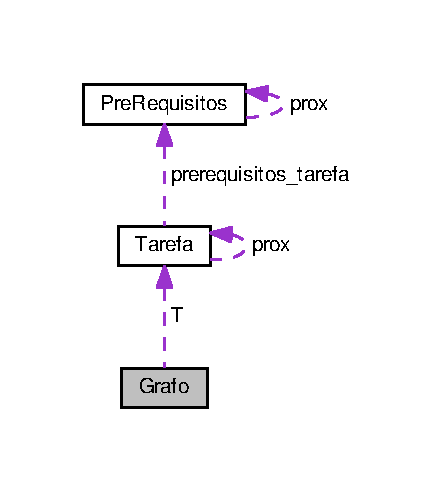
\includegraphics[width=208pt]{structGrafo__coll__graph}
\end{center}
\end{figure}
\subsection*{Atributos Públicos}
\begin{DoxyCompactItemize}
\item 
\hyperlink{grafo_8h_ab156210f10bb550f6d61bea964f08c22}{tarefa} $\ast$ \hyperlink{structGrafo_aeb37989f62bb38c1b5ebce8bfa63ad32}{T}
\end{DoxyCompactItemize}


\subsection{Documentação dos dados membro}
\hypertarget{structGrafo_aeb37989f62bb38c1b5ebce8bfa63ad32}{\index{Grafo@{Grafo}!T@{T}}
\index{T@{T}!Grafo@{Grafo}}
\subsubsection[{T}]{\setlength{\rightskip}{0pt plus 5cm}{\bf tarefa}$\ast$ Grafo\-::\-T}}\label{structGrafo_aeb37989f62bb38c1b5ebce8bfa63ad32}


A documentação para esta estrutura foi gerada a partir do seguinte ficheiro\-:\begin{DoxyCompactItemize}
\item 
include/\hyperlink{grafo_8h}{grafo.\-h}\end{DoxyCompactItemize}

\hypertarget{classtesting_1_1internal_1_1GTestFlagSaver}{\section{Referência à classe testing\-:\-:internal\-:\-:G\-Test\-Flag\-Saver}
\label{classtesting_1_1internal_1_1GTestFlagSaver}\index{testing\-::internal\-::\-G\-Test\-Flag\-Saver@{testing\-::internal\-::\-G\-Test\-Flag\-Saver}}
}


A documentação para esta classe foi gerada a partir do seguinte ficheiro\-:\begin{DoxyCompactItemize}
\item 
src/gtest-\/internal-\/inl.\-h\end{DoxyCompactItemize}

\hypertarget{classtesting_1_1internal_1_1GTestLog}{\section{Referência à classe testing\-:\-:internal\-:\-:G\-Test\-Log}
\label{classtesting_1_1internal_1_1GTestLog}\index{testing\-::internal\-::\-G\-Test\-Log@{testing\-::internal\-::\-G\-Test\-Log}}
}
\subsection*{Membros públicos}
\begin{DoxyCompactItemize}
\item 
\hypertarget{classtesting_1_1internal_1_1GTestLog_a364691bf972983a59cfa2891062a64af}{{\bfseries G\-Test\-Log} (G\-Test\-Log\-Severity severity, const char $\ast$file, int line)}\label{classtesting_1_1internal_1_1GTestLog_a364691bf972983a59cfa2891062a64af}

\item 
\hypertarget{classtesting_1_1internal_1_1GTestLog_aebb92e67d98eca69f0347d5121dab27a}{\-::std\-::ostream \& {\bfseries Get\-Stream} ()}\label{classtesting_1_1internal_1_1GTestLog_aebb92e67d98eca69f0347d5121dab27a}

\end{DoxyCompactItemize}


A documentação para esta classe foi gerada a partir dos seguintes ficheiros\-:\begin{DoxyCompactItemize}
\item 
include/gtest/internal/gtest-\/port.\-h\item 
src/gtest-\/port.\-cc\end{DoxyCompactItemize}

\hypertarget{classtesting_1_1internal_1_1GTestMutexLock}{\section{Referência à classe testing\-:\-:internal\-:\-:G\-Test\-Mutex\-Lock}
\label{classtesting_1_1internal_1_1GTestMutexLock}\index{testing\-::internal\-::\-G\-Test\-Mutex\-Lock@{testing\-::internal\-::\-G\-Test\-Mutex\-Lock}}
}
\subsection*{Membros públicos}
\begin{DoxyCompactItemize}
\item 
\hypertarget{classtesting_1_1internal_1_1GTestMutexLock_a77e3cba326d5356b4a1dea3790559c26}{{\bfseries G\-Test\-Mutex\-Lock} (\hyperlink{classtesting_1_1internal_1_1Mutex}{Mutex} $\ast$)}\label{classtesting_1_1internal_1_1GTestMutexLock_a77e3cba326d5356b4a1dea3790559c26}

\end{DoxyCompactItemize}


A documentação para esta classe foi gerada a partir do seguinte ficheiro\-:\begin{DoxyCompactItemize}
\item 
include/gtest/internal/gtest-\/port.\-h\end{DoxyCompactItemize}

\hypertarget{classtesting_1_1internal_1_1HasNewFatalFailureHelper}{\section{Referência à classe testing\-:\-:internal\-:\-:Has\-New\-Fatal\-Failure\-Helper}
\label{classtesting_1_1internal_1_1HasNewFatalFailureHelper}\index{testing\-::internal\-::\-Has\-New\-Fatal\-Failure\-Helper@{testing\-::internal\-::\-Has\-New\-Fatal\-Failure\-Helper}}
}
Diagrama de heranças da classe testing\-:\-:internal\-:\-:Has\-New\-Fatal\-Failure\-Helper\begin{figure}[H]
\begin{center}
\leavevmode
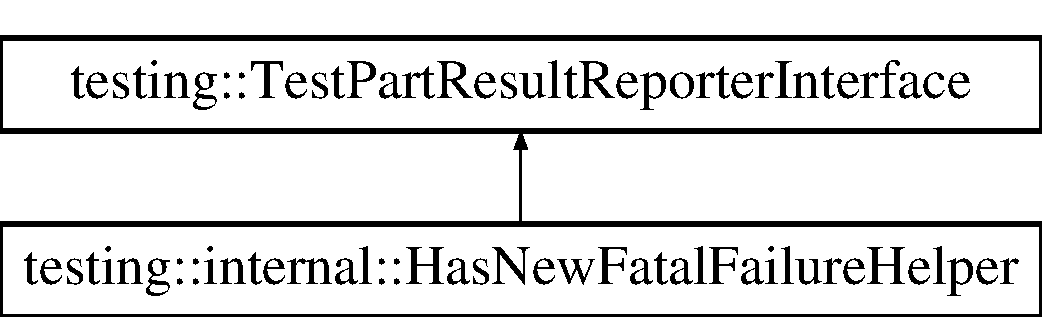
\includegraphics[height=2.000000cm]{classtesting_1_1internal_1_1HasNewFatalFailureHelper}
\end{center}
\end{figure}
\subsection*{Membros públicos}
\begin{DoxyCompactItemize}
\item 
\hypertarget{classtesting_1_1internal_1_1HasNewFatalFailureHelper_a2d2e1faa1f3669b82810df97ac678a27}{virtual void {\bfseries Report\-Test\-Part\-Result} (const \hyperlink{classtesting_1_1TestPartResult}{Test\-Part\-Result} \&result)}\label{classtesting_1_1internal_1_1HasNewFatalFailureHelper_a2d2e1faa1f3669b82810df97ac678a27}

\item 
\hypertarget{classtesting_1_1internal_1_1HasNewFatalFailureHelper_ae137e639098071f11f531bbd72dde1c7}{bool {\bfseries has\-\_\-new\-\_\-fatal\-\_\-failure} () const }\label{classtesting_1_1internal_1_1HasNewFatalFailureHelper_ae137e639098071f11f531bbd72dde1c7}

\end{DoxyCompactItemize}


A documentação para esta classe foi gerada a partir dos seguintes ficheiros\-:\begin{DoxyCompactItemize}
\item 
include/gtest/gtest-\/test-\/part.\-h\item 
src/gtest-\/test-\/part.\-cc\end{DoxyCompactItemize}

\hypertarget{classtesting_1_1internal_1_1ImplicitlyConvertible}{\section{Referência à classe Template testing\-:\-:internal\-:\-:Implicitly\-Convertible$<$ From, To $>$}
\label{classtesting_1_1internal_1_1ImplicitlyConvertible}\index{testing\-::internal\-::\-Implicitly\-Convertible$<$ From, To $>$@{testing\-::internal\-::\-Implicitly\-Convertible$<$ From, To $>$}}
}
\subsection*{Atributos Públicos Estáticos}
\begin{DoxyCompactItemize}
\item 
static const bool {\bfseries value}
\end{DoxyCompactItemize}


\subsection{Documentação dos dados membro}
\hypertarget{classtesting_1_1internal_1_1ImplicitlyConvertible_aea51cecabca681fb75659e224771b7b7}{\index{testing\-::internal\-::\-Implicitly\-Convertible@{testing\-::internal\-::\-Implicitly\-Convertible}!value@{value}}
\index{value@{value}!testing::internal::ImplicitlyConvertible@{testing\-::internal\-::\-Implicitly\-Convertible}}
\subsubsection[{value}]{\setlength{\rightskip}{0pt plus 5cm}template$<$typename From , typename To $>$ const bool {\bf testing\-::internal\-::\-Implicitly\-Convertible}$<$ From, To $>$\-::value\hspace{0.3cm}{\ttfamily [static]}}}\label{classtesting_1_1internal_1_1ImplicitlyConvertible_aea51cecabca681fb75659e224771b7b7}
{\bfseries Valor inicial\-:}
\begin{DoxyCode}
=
      \textcolor{keyword}{sizeof}(Helper(ImplicitlyConvertible::MakeFrom())) == 1
\end{DoxyCode}


A documentação para esta classe foi gerada a partir do seguinte ficheiro\-:\begin{DoxyCompactItemize}
\item 
include/gtest/internal/gtest-\/internal.\-h\end{DoxyCompactItemize}

\hypertarget{structtesting_1_1internal_1_1is__pointer}{\section{Referência à estrutura Template testing\-:\-:internal\-:\-:is\-\_\-pointer$<$ T $>$}
\label{structtesting_1_1internal_1_1is__pointer}\index{testing\-::internal\-::is\-\_\-pointer$<$ T $>$@{testing\-::internal\-::is\-\_\-pointer$<$ T $>$}}
}
Diagrama de heranças da classe testing\-:\-:internal\-:\-:is\-\_\-pointer$<$ T $>$\begin{figure}[H]
\begin{center}
\leavevmode
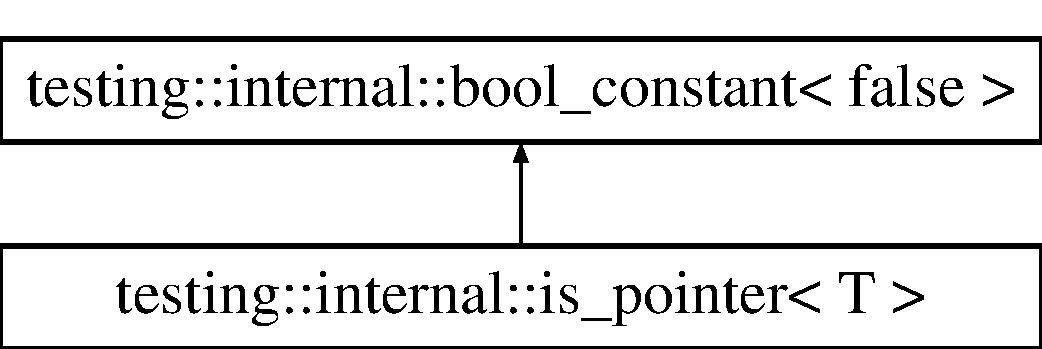
\includegraphics[height=2.000000cm]{structtesting_1_1internal_1_1is__pointer}
\end{center}
\end{figure}
\subsection*{Additional Inherited Members}


A documentação para esta estrutura foi gerada a partir do seguinte ficheiro\-:\begin{DoxyCompactItemize}
\item 
include/gtest/internal/gtest-\/port.\-h\end{DoxyCompactItemize}

\hypertarget{structtesting_1_1internal_1_1is__pointer_3_01T_01_5_01_4}{\section{Referência à estrutura Template testing\-:\-:internal\-:\-:is\-\_\-pointer$<$ T $\ast$ $>$}
\label{structtesting_1_1internal_1_1is__pointer_3_01T_01_5_01_4}\index{testing\-::internal\-::is\-\_\-pointer$<$ T $\ast$ $>$@{testing\-::internal\-::is\-\_\-pointer$<$ T $\ast$ $>$}}
}
Diagrama de heranças da classe testing\-:\-:internal\-:\-:is\-\_\-pointer$<$ T $\ast$ $>$\begin{figure}[H]
\begin{center}
\leavevmode
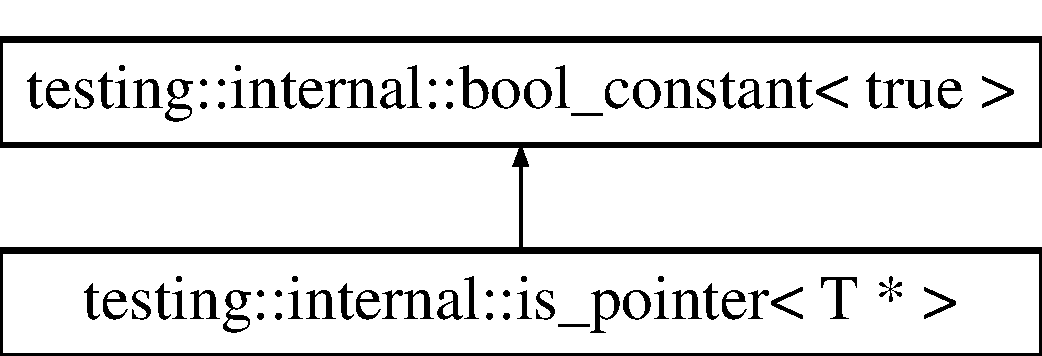
\includegraphics[height=2.000000cm]{structtesting_1_1internal_1_1is__pointer_3_01T_01_5_01_4}
\end{center}
\end{figure}
\subsection*{Additional Inherited Members}


A documentação para esta estrutura foi gerada a partir do seguinte ficheiro\-:\begin{DoxyCompactItemize}
\item 
include/gtest/internal/gtest-\/port.\-h\end{DoxyCompactItemize}

\hypertarget{structtesting_1_1internal_1_1IsAProtocolMessage}{\section{Referência à estrutura Template testing\-:\-:internal\-:\-:Is\-A\-Protocol\-Message$<$ T $>$}
\label{structtesting_1_1internal_1_1IsAProtocolMessage}\index{testing\-::internal\-::\-Is\-A\-Protocol\-Message$<$ T $>$@{testing\-::internal\-::\-Is\-A\-Protocol\-Message$<$ T $>$}}
}
Diagrama de heranças da classe testing\-:\-:internal\-:\-:Is\-A\-Protocol\-Message$<$ T $>$\begin{figure}[H]
\begin{center}
\leavevmode
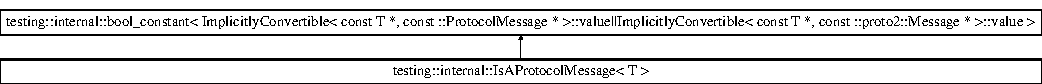
\includegraphics[height=1.132457cm]{structtesting_1_1internal_1_1IsAProtocolMessage}
\end{center}
\end{figure}
\subsection*{Additional Inherited Members}


A documentação para esta estrutura foi gerada a partir do seguinte ficheiro\-:\begin{DoxyCompactItemize}
\item 
include/gtest/internal/gtest-\/internal.\-h\end{DoxyCompactItemize}

\hypertarget{structtesting_1_1internal_1_1IteratorTraits}{\section{Referência à estrutura Template testing\-:\-:internal\-:\-:Iterator\-Traits$<$ Iterator $>$}
\label{structtesting_1_1internal_1_1IteratorTraits}\index{testing\-::internal\-::\-Iterator\-Traits$<$ Iterator $>$@{testing\-::internal\-::\-Iterator\-Traits$<$ Iterator $>$}}
}
\subsection*{Tipos Públicos}
\begin{DoxyCompactItemize}
\item 
\hypertarget{structtesting_1_1internal_1_1IteratorTraits_a29de4320a9c53ce438d3561b94e515bb}{typedef Iterator\-::value\-\_\-type {\bfseries value\-\_\-type}}\label{structtesting_1_1internal_1_1IteratorTraits_a29de4320a9c53ce438d3561b94e515bb}

\end{DoxyCompactItemize}


A documentação para esta estrutura foi gerada a partir do seguinte ficheiro\-:\begin{DoxyCompactItemize}
\item 
include/gtest/internal/gtest-\/port.\-h\end{DoxyCompactItemize}

\hypertarget{structtesting_1_1internal_1_1IteratorTraits_3_01const_01T_01_5_01_4}{\section{Referência à estrutura Template testing\-:\-:internal\-:\-:Iterator\-Traits$<$ const T $\ast$ $>$}
\label{structtesting_1_1internal_1_1IteratorTraits_3_01const_01T_01_5_01_4}\index{testing\-::internal\-::\-Iterator\-Traits$<$ const T $\ast$ $>$@{testing\-::internal\-::\-Iterator\-Traits$<$ const T $\ast$ $>$}}
}
\subsection*{Tipos Públicos}
\begin{DoxyCompactItemize}
\item 
\hypertarget{structtesting_1_1internal_1_1IteratorTraits_3_01const_01T_01_5_01_4_ae7c8867223e106f374b56a7dc4a85547}{typedef T {\bfseries value\-\_\-type}}\label{structtesting_1_1internal_1_1IteratorTraits_3_01const_01T_01_5_01_4_ae7c8867223e106f374b56a7dc4a85547}

\end{DoxyCompactItemize}


A documentação para esta estrutura foi gerada a partir do seguinte ficheiro\-:\begin{DoxyCompactItemize}
\item 
include/gtest/internal/gtest-\/port.\-h\end{DoxyCompactItemize}

\hypertarget{structtesting_1_1internal_1_1IteratorTraits_3_01T_01_5_01_4}{\section{Referência à estrutura Template testing\-:\-:internal\-:\-:Iterator\-Traits$<$ T $\ast$ $>$}
\label{structtesting_1_1internal_1_1IteratorTraits_3_01T_01_5_01_4}\index{testing\-::internal\-::\-Iterator\-Traits$<$ T $\ast$ $>$@{testing\-::internal\-::\-Iterator\-Traits$<$ T $\ast$ $>$}}
}
\subsection*{Tipos Públicos}
\begin{DoxyCompactItemize}
\item 
\hypertarget{structtesting_1_1internal_1_1IteratorTraits_3_01T_01_5_01_4_a7e46869ed36cc5aea898e243d270a8be}{typedef T {\bfseries value\-\_\-type}}\label{structtesting_1_1internal_1_1IteratorTraits_3_01T_01_5_01_4_a7e46869ed36cc5aea898e243d270a8be}

\end{DoxyCompactItemize}


A documentação para esta estrutura foi gerada a partir do seguinte ficheiro\-:\begin{DoxyCompactItemize}
\item 
include/gtest/internal/gtest-\/port.\-h\end{DoxyCompactItemize}

\hypertarget{classtesting_1_1internal_1_1linked__ptr}{\section{Referência à classe Template testing\-:\-:internal\-:\-:linked\-\_\-ptr$<$ T $>$}
\label{classtesting_1_1internal_1_1linked__ptr}\index{testing\-::internal\-::linked\-\_\-ptr$<$ T $>$@{testing\-::internal\-::linked\-\_\-ptr$<$ T $>$}}
}
\subsection*{Tipos Públicos}
\begin{DoxyCompactItemize}
\item 
\hypertarget{classtesting_1_1internal_1_1linked__ptr_a295c7d1ee4100d916514c4e4385a0063}{typedef T {\bfseries element\-\_\-type}}\label{classtesting_1_1internal_1_1linked__ptr_a295c7d1ee4100d916514c4e4385a0063}

\end{DoxyCompactItemize}
\subsection*{Membros públicos}
\begin{DoxyCompactItemize}
\item 
\hypertarget{classtesting_1_1internal_1_1linked__ptr_ae805418b9f03f14ff49649e710475dba}{{\bfseries linked\-\_\-ptr} (T $\ast$ptr=N\-U\-L\-L)}\label{classtesting_1_1internal_1_1linked__ptr_ae805418b9f03f14ff49649e710475dba}

\item 
\hypertarget{classtesting_1_1internal_1_1linked__ptr_a7597ed91006edd0467c99bd1aaab07f5}{{\footnotesize template$<$typename U $>$ }\\{\bfseries linked\-\_\-ptr} (\hyperlink{classtesting_1_1internal_1_1linked__ptr}{linked\-\_\-ptr}$<$ U $>$ const \&ptr)}\label{classtesting_1_1internal_1_1linked__ptr_a7597ed91006edd0467c99bd1aaab07f5}

\item 
\hypertarget{classtesting_1_1internal_1_1linked__ptr_abc076b5678cc7f64306d5ecfefc93aff}{{\bfseries linked\-\_\-ptr} (\hyperlink{classtesting_1_1internal_1_1linked__ptr}{linked\-\_\-ptr} const \&ptr)}\label{classtesting_1_1internal_1_1linked__ptr_abc076b5678cc7f64306d5ecfefc93aff}

\item 
\hypertarget{classtesting_1_1internal_1_1linked__ptr_a82608d98869b750d9ab729f1450a9a45}{{\footnotesize template$<$typename U $>$ }\\\hyperlink{classtesting_1_1internal_1_1linked__ptr}{linked\-\_\-ptr} \& {\bfseries operator=} (\hyperlink{classtesting_1_1internal_1_1linked__ptr}{linked\-\_\-ptr}$<$ U $>$ const \&ptr)}\label{classtesting_1_1internal_1_1linked__ptr_a82608d98869b750d9ab729f1450a9a45}

\item 
\hypertarget{classtesting_1_1internal_1_1linked__ptr_a1f40b5e66e6cf7b661ea116c806f952e}{\hyperlink{classtesting_1_1internal_1_1linked__ptr}{linked\-\_\-ptr} \& {\bfseries operator=} (\hyperlink{classtesting_1_1internal_1_1linked__ptr}{linked\-\_\-ptr} const \&ptr)}\label{classtesting_1_1internal_1_1linked__ptr_a1f40b5e66e6cf7b661ea116c806f952e}

\item 
\hypertarget{classtesting_1_1internal_1_1linked__ptr_a95ba3b7b66ed0193c779976c6e126ab6}{void {\bfseries reset} (T $\ast$ptr=N\-U\-L\-L)}\label{classtesting_1_1internal_1_1linked__ptr_a95ba3b7b66ed0193c779976c6e126ab6}

\item 
\hypertarget{classtesting_1_1internal_1_1linked__ptr_a6ea8584d9bcad13c3266834f5ce5e771}{T $\ast$ {\bfseries get} () const }\label{classtesting_1_1internal_1_1linked__ptr_a6ea8584d9bcad13c3266834f5ce5e771}

\item 
\hypertarget{classtesting_1_1internal_1_1linked__ptr_aa878c3e874242fb3cd2aa14ec603aa25}{T $\ast$ {\bfseries operator-\/$>$} () const }\label{classtesting_1_1internal_1_1linked__ptr_aa878c3e874242fb3cd2aa14ec603aa25}

\item 
\hypertarget{classtesting_1_1internal_1_1linked__ptr_aec393cbd60f96defde36ef8a69d94254}{T \& {\bfseries operator$\ast$} () const }\label{classtesting_1_1internal_1_1linked__ptr_aec393cbd60f96defde36ef8a69d94254}

\item 
\hypertarget{classtesting_1_1internal_1_1linked__ptr_abe2154fd3ad3574dfe6f2320bc1debc4}{bool {\bfseries operator==} (T $\ast$p) const }\label{classtesting_1_1internal_1_1linked__ptr_abe2154fd3ad3574dfe6f2320bc1debc4}

\item 
\hypertarget{classtesting_1_1internal_1_1linked__ptr_a3685f9661bbe410cfa58fea2f14396b7}{bool {\bfseries operator!=} (T $\ast$p) const }\label{classtesting_1_1internal_1_1linked__ptr_a3685f9661bbe410cfa58fea2f14396b7}

\item 
\hypertarget{classtesting_1_1internal_1_1linked__ptr_a3b46c9ecfd928673a524dcb3c70fd2ad}{{\footnotesize template$<$typename U $>$ }\\bool {\bfseries operator==} (\hyperlink{classtesting_1_1internal_1_1linked__ptr}{linked\-\_\-ptr}$<$ U $>$ const \&ptr) const }\label{classtesting_1_1internal_1_1linked__ptr_a3b46c9ecfd928673a524dcb3c70fd2ad}

\item 
\hypertarget{classtesting_1_1internal_1_1linked__ptr_a6449584b90a09a313300599fb3a23633}{{\footnotesize template$<$typename U $>$ }\\bool {\bfseries operator!=} (\hyperlink{classtesting_1_1internal_1_1linked__ptr}{linked\-\_\-ptr}$<$ U $>$ const \&ptr) const }\label{classtesting_1_1internal_1_1linked__ptr_a6449584b90a09a313300599fb3a23633}

\end{DoxyCompactItemize}
\subsection*{Amigos}
\begin{DoxyCompactItemize}
\item 
\hypertarget{classtesting_1_1internal_1_1linked__ptr_a7763f286ca03a7f7363a033d996c8c1c}{{\footnotesize template$<$typename U $>$ }\\class {\bfseries linked\-\_\-ptr}}\label{classtesting_1_1internal_1_1linked__ptr_a7763f286ca03a7f7363a033d996c8c1c}

\end{DoxyCompactItemize}


A documentação para esta classe foi gerada a partir do seguinte ficheiro\-:\begin{DoxyCompactItemize}
\item 
include/gtest/internal/gtest-\/linked\-\_\-ptr.\-h\end{DoxyCompactItemize}

\hypertarget{classtesting_1_1internal_1_1linked__ptr__internal}{\section{Referência à classe testing\-:\-:internal\-:\-:linked\-\_\-ptr\-\_\-internal}
\label{classtesting_1_1internal_1_1linked__ptr__internal}\index{testing\-::internal\-::linked\-\_\-ptr\-\_\-internal@{testing\-::internal\-::linked\-\_\-ptr\-\_\-internal}}
}
\subsection*{Membros públicos}
\begin{DoxyCompactItemize}
\item 
\hypertarget{classtesting_1_1internal_1_1linked__ptr__internal_a742af1f65df2d5e2b7198a1b74264a83}{void {\bfseries join\-\_\-new} ()}\label{classtesting_1_1internal_1_1linked__ptr__internal_a742af1f65df2d5e2b7198a1b74264a83}

\item 
\hypertarget{classtesting_1_1internal_1_1linked__ptr__internal_acd5a341459f7e81b10b4112d8c764e2a}{void {\bfseries join} (\hyperlink{classtesting_1_1internal_1_1linked__ptr__internal}{linked\-\_\-ptr\-\_\-internal} const $\ast$ptr) G\-T\-E\-S\-T\-\_\-\-L\-O\-C\-K\-\_\-\-E\-X\-C\-L\-U\-D\-E\-D\-\_\-(g\-\_\-linked\-\_\-ptr\-\_\-mutex)}\label{classtesting_1_1internal_1_1linked__ptr__internal_acd5a341459f7e81b10b4112d8c764e2a}

\item 
\hypertarget{classtesting_1_1internal_1_1linked__ptr__internal_a8699e539d9702d363ef0351012d1b3ca}{bool {\bfseries depart} () G\-T\-E\-S\-T\-\_\-\-L\-O\-C\-K\-\_\-\-E\-X\-C\-L\-U\-D\-E\-D\-\_\-(g\-\_\-linked\-\_\-ptr\-\_\-mutex)}\label{classtesting_1_1internal_1_1linked__ptr__internal_a8699e539d9702d363ef0351012d1b3ca}

\end{DoxyCompactItemize}


A documentação para esta classe foi gerada a partir do seguinte ficheiro\-:\begin{DoxyCompactItemize}
\item 
include/gtest/internal/gtest-\/linked\-\_\-ptr.\-h\end{DoxyCompactItemize}

\hypertarget{structLISTA}{\section{Referência à estrutura L\-I\-S\-T\-A}
\label{structLISTA}\index{L\-I\-S\-T\-A@{L\-I\-S\-T\-A}}
}
\subsection*{Atributos Públicos}
\begin{DoxyCompactItemize}
\item 
int \hyperlink{structLISTA_a81b29c44560db14d9d5ef75858c91a0b}{t}
\item 
struct \hyperlink{structLISTA}{L\-I\-S\-T\-A} $\ast$ \hyperlink{structLISTA_a818a9fbd5f34b29597c140c052309ea6}{prox}
\item 
struct \hyperlink{structLISTA}{L\-I\-S\-T\-A} $\ast$ \hyperlink{structLISTA_acbab5a56fa16181657e3036ffa9fca11}{ant}
\end{DoxyCompactItemize}


\subsection{Documentação dos dados membro}
\hypertarget{structLISTA_acbab5a56fa16181657e3036ffa9fca11}{\index{L\-I\-S\-T\-A@{L\-I\-S\-T\-A}!ant@{ant}}
\index{ant@{ant}!LISTA@{L\-I\-S\-T\-A}}
\subsubsection[{ant}]{\setlength{\rightskip}{0pt plus 5cm}struct {\bf L\-I\-S\-T\-A} $\ast$ L\-I\-S\-T\-A\-::ant}}\label{structLISTA_acbab5a56fa16181657e3036ffa9fca11}
\hypertarget{structLISTA_a818a9fbd5f34b29597c140c052309ea6}{\index{L\-I\-S\-T\-A@{L\-I\-S\-T\-A}!prox@{prox}}
\index{prox@{prox}!LISTA@{L\-I\-S\-T\-A}}
\subsubsection[{prox}]{\setlength{\rightskip}{0pt plus 5cm}struct {\bf L\-I\-S\-T\-A}$\ast$ L\-I\-S\-T\-A\-::prox}}\label{structLISTA_a818a9fbd5f34b29597c140c052309ea6}
\hypertarget{structLISTA_a81b29c44560db14d9d5ef75858c91a0b}{\index{L\-I\-S\-T\-A@{L\-I\-S\-T\-A}!t@{t}}
\index{t@{t}!LISTA@{L\-I\-S\-T\-A}}
\subsubsection[{t}]{\setlength{\rightskip}{0pt plus 5cm}int L\-I\-S\-T\-A\-::t}}\label{structLISTA_a81b29c44560db14d9d5ef75858c91a0b}


A documentação para esta estrutura foi gerada a partir do seguinte ficheiro\-:\begin{DoxyCompactItemize}
\item 
code/\hyperlink{grafo_8cc}{grafo.\-cc}\end{DoxyCompactItemize}

\hypertarget{classtesting_1_1Message}{\section{Referência à classe testing\-:\-:Message}
\label{classtesting_1_1Message}\index{testing\-::\-Message@{testing\-::\-Message}}
}
\subsection*{Membros públicos}
\begin{DoxyCompactItemize}
\item 
\hypertarget{classtesting_1_1Message_ac126e24804817a053bebba0920d94a11}{{\bfseries Message} (const \hyperlink{classtesting_1_1Message}{Message} \&msg)}\label{classtesting_1_1Message_ac126e24804817a053bebba0920d94a11}

\item 
\hypertarget{classtesting_1_1Message_a9de694ca239486809fc99fbbea8ac21d}{{\bfseries Message} (const char $\ast$str)}\label{classtesting_1_1Message_a9de694ca239486809fc99fbbea8ac21d}

\item 
\hypertarget{classtesting_1_1Message_a2e0e71be52d54c20a75a55fca812721f}{{\footnotesize template$<$typename T $>$ }\\\hyperlink{classtesting_1_1Message}{Message} \& {\bfseries operator$<$$<$} (const T \&val)}\label{classtesting_1_1Message_a2e0e71be52d54c20a75a55fca812721f}

\item 
\hypertarget{classtesting_1_1Message_aa3ab685879958f90d2d8cd5b68d10c34}{{\footnotesize template$<$typename T $>$ }\\\hyperlink{classtesting_1_1Message}{Message} \& {\bfseries operator$<$$<$} (T $\ast$const \&pointer)}\label{classtesting_1_1Message_aa3ab685879958f90d2d8cd5b68d10c34}

\item 
\hypertarget{classtesting_1_1Message_a3a71a1c1c8ea52de5852d75483d41453}{\hyperlink{classtesting_1_1Message}{Message} \& {\bfseries operator$<$$<$} (Basic\-Narrow\-Io\-Manip val)}\label{classtesting_1_1Message_a3a71a1c1c8ea52de5852d75483d41453}

\item 
\hypertarget{classtesting_1_1Message_a3e1e04f23b1bdfe18adfd59928296346}{\hyperlink{classtesting_1_1Message}{Message} \& {\bfseries operator$<$$<$} (bool b)}\label{classtesting_1_1Message_a3e1e04f23b1bdfe18adfd59928296346}

\item 
\hypertarget{classtesting_1_1Message_ac0db9c22535b28bc863bfd0a1fdf7e14}{\hyperlink{classtesting_1_1Message}{Message} \& {\bfseries operator$<$$<$} (const wchar\-\_\-t $\ast$wide\-\_\-c\-\_\-str)}\label{classtesting_1_1Message_ac0db9c22535b28bc863bfd0a1fdf7e14}

\item 
\hypertarget{classtesting_1_1Message_ac1d3a041ac4bb9c929ee746b31a13d6a}{\hyperlink{classtesting_1_1Message}{Message} \& {\bfseries operator$<$$<$} (wchar\-\_\-t $\ast$wide\-\_\-c\-\_\-str)}\label{classtesting_1_1Message_ac1d3a041ac4bb9c929ee746b31a13d6a}

\item 
\hypertarget{classtesting_1_1Message_abe8c1b7584aa670dd0e2413e8317a937}{std\-::string {\bfseries Get\-String} () const }\label{classtesting_1_1Message_abe8c1b7584aa670dd0e2413e8317a937}

\end{DoxyCompactItemize}


A documentação para esta classe foi gerada a partir dos seguintes ficheiros\-:\begin{DoxyCompactItemize}
\item 
include/gtest/gtest-\/message.\-h\item 
src/gtest.\-cc\end{DoxyCompactItemize}

\hypertarget{classtesting_1_1internal_1_1Mutex}{\section{Referência à classe testing\-:\-:internal\-:\-:Mutex}
\label{classtesting_1_1internal_1_1Mutex}\index{testing\-::internal\-::\-Mutex@{testing\-::internal\-::\-Mutex}}
}
\subsection*{Membros públicos}
\begin{DoxyCompactItemize}
\item 
\hypertarget{classtesting_1_1internal_1_1Mutex_ae7e2191886c00182176b23c4f4d049f8}{void {\bfseries Lock} ()}\label{classtesting_1_1internal_1_1Mutex_ae7e2191886c00182176b23c4f4d049f8}

\item 
\hypertarget{classtesting_1_1internal_1_1Mutex_a315188055de1be98884519ad84eff2e6}{void {\bfseries Unlock} ()}\label{classtesting_1_1internal_1_1Mutex_a315188055de1be98884519ad84eff2e6}

\item 
\hypertarget{classtesting_1_1internal_1_1Mutex_a3a0530bca3110025d85b2aa51f3ca0d7}{void {\bfseries Assert\-Held} () const }\label{classtesting_1_1internal_1_1Mutex_a3a0530bca3110025d85b2aa51f3ca0d7}

\end{DoxyCompactItemize}


A documentação para esta classe foi gerada a partir do seguinte ficheiro\-:\begin{DoxyCompactItemize}
\item 
include/gtest/internal/gtest-\/port.\-h\end{DoxyCompactItemize}

\hypertarget{classtesting_1_1internal_1_1NativeArray}{\section{Referência à classe Template testing\-:\-:internal\-:\-:Native\-Array$<$ Element $>$}
\label{classtesting_1_1internal_1_1NativeArray}\index{testing\-::internal\-::\-Native\-Array$<$ Element $>$@{testing\-::internal\-::\-Native\-Array$<$ Element $>$}}
}
\subsection*{Tipos Públicos}
\begin{DoxyCompactItemize}
\item 
\hypertarget{classtesting_1_1internal_1_1NativeArray_a12216d686e16e4cc63d952fada5b2ba9}{typedef Element {\bfseries value\-\_\-type}}\label{classtesting_1_1internal_1_1NativeArray_a12216d686e16e4cc63d952fada5b2ba9}

\item 
\hypertarget{classtesting_1_1internal_1_1NativeArray_ac1301a57977b57a1ad013e4e25fc2a72}{typedef Element $\ast$ {\bfseries iterator}}\label{classtesting_1_1internal_1_1NativeArray_ac1301a57977b57a1ad013e4e25fc2a72}

\item 
\hypertarget{classtesting_1_1internal_1_1NativeArray_a9ce7c8408460d7158a2870456d134557}{typedef const Element $\ast$ {\bfseries const\-\_\-iterator}}\label{classtesting_1_1internal_1_1NativeArray_a9ce7c8408460d7158a2870456d134557}

\end{DoxyCompactItemize}
\subsection*{Membros públicos}
\begin{DoxyCompactItemize}
\item 
\hypertarget{classtesting_1_1internal_1_1NativeArray_a568de999aca0fc0c2cc574fac2405872}{{\bfseries Native\-Array} (const Element $\ast$array, size\-\_\-t count, Relation\-To\-Source relation)}\label{classtesting_1_1internal_1_1NativeArray_a568de999aca0fc0c2cc574fac2405872}

\item 
\hypertarget{classtesting_1_1internal_1_1NativeArray_abb346ac3040f5da733f594cc2d5958bc}{{\bfseries Native\-Array} (const \hyperlink{classtesting_1_1internal_1_1NativeArray}{Native\-Array} \&rhs)}\label{classtesting_1_1internal_1_1NativeArray_abb346ac3040f5da733f594cc2d5958bc}

\item 
\hypertarget{classtesting_1_1internal_1_1NativeArray_a45de2485baac8bf148e2943828094a40}{size\-\_\-t {\bfseries size} () const }\label{classtesting_1_1internal_1_1NativeArray_a45de2485baac8bf148e2943828094a40}

\item 
\hypertarget{classtesting_1_1internal_1_1NativeArray_a49c534d29034d9230372ada54ef961bb}{const\-\_\-iterator {\bfseries begin} () const }\label{classtesting_1_1internal_1_1NativeArray_a49c534d29034d9230372ada54ef961bb}

\item 
\hypertarget{classtesting_1_1internal_1_1NativeArray_a4957ad1ebf7c21eab07d5e0ae2bb17aa}{const\-\_\-iterator {\bfseries end} () const }\label{classtesting_1_1internal_1_1NativeArray_a4957ad1ebf7c21eab07d5e0ae2bb17aa}

\item 
\hypertarget{classtesting_1_1internal_1_1NativeArray_a60af8d9c429771ee131b5ddf7e06e3c9}{bool {\bfseries operator==} (const \hyperlink{classtesting_1_1internal_1_1NativeArray}{Native\-Array} \&rhs) const }\label{classtesting_1_1internal_1_1NativeArray_a60af8d9c429771ee131b5ddf7e06e3c9}

\end{DoxyCompactItemize}


A documentação para esta classe foi gerada a partir do seguinte ficheiro\-:\begin{DoxyCompactItemize}
\item 
include/gtest/internal/gtest-\/internal.\-h\end{DoxyCompactItemize}

\hypertarget{classtesting_1_1internal_1_1OsStackTraceGetter}{\section{Referência à classe testing\-:\-:internal\-:\-:Os\-Stack\-Trace\-Getter}
\label{classtesting_1_1internal_1_1OsStackTraceGetter}\index{testing\-::internal\-::\-Os\-Stack\-Trace\-Getter@{testing\-::internal\-::\-Os\-Stack\-Trace\-Getter}}
}
Diagrama de heranças da classe testing\-:\-:internal\-:\-:Os\-Stack\-Trace\-Getter\begin{figure}[H]
\begin{center}
\leavevmode
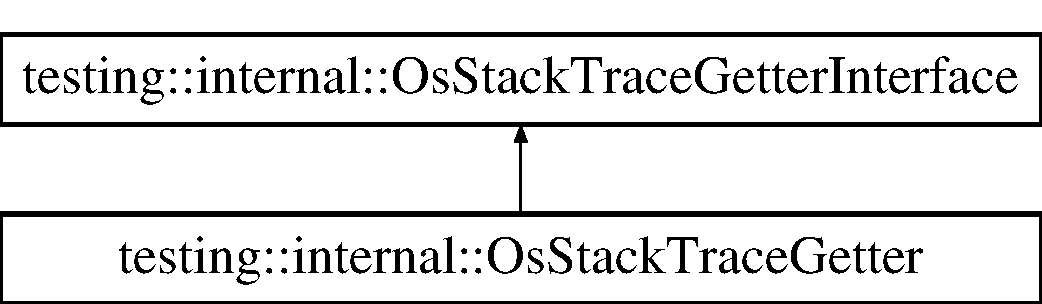
\includegraphics[height=2.000000cm]{classtesting_1_1internal_1_1OsStackTraceGetter}
\end{center}
\end{figure}
\subsection*{Membros públicos}
\begin{DoxyCompactItemize}
\item 
\hypertarget{classtesting_1_1internal_1_1OsStackTraceGetter_afe0f7539f1a325eec1adf0625bbdfbd7}{virtual string {\bfseries Current\-Stack\-Trace} (int max\-\_\-depth, int skip\-\_\-count) G\-T\-E\-S\-T\-\_\-\-L\-O\-C\-K\-\_\-\-E\-X\-C\-L\-U\-D\-E\-D\-\_\-(mutex\-\_\-)}\label{classtesting_1_1internal_1_1OsStackTraceGetter_afe0f7539f1a325eec1adf0625bbdfbd7}

\item 
\hypertarget{classtesting_1_1internal_1_1OsStackTraceGetter_abdfefeba8ffb0f1031491e4bd1a7fad9}{virtual void {\bfseries Upon\-Leaving\-G\-Test} () G\-T\-E\-S\-T\-\_\-\-L\-O\-C\-K\-\_\-\-E\-X\-C\-L\-U\-D\-E\-D\-\_\-(mutex\-\_\-)}\label{classtesting_1_1internal_1_1OsStackTraceGetter_abdfefeba8ffb0f1031491e4bd1a7fad9}

\end{DoxyCompactItemize}
\subsection*{Atributos Públicos Estáticos}
\begin{DoxyCompactItemize}
\item 
static const char $\ast$const {\bfseries k\-Elided\-Frames\-Marker}
\end{DoxyCompactItemize}


\subsection{Documentação dos dados membro}
\hypertarget{classtesting_1_1internal_1_1OsStackTraceGetter_aa736c26a4ba2b59a7572e7f44bfe269e}{\index{testing\-::internal\-::\-Os\-Stack\-Trace\-Getter@{testing\-::internal\-::\-Os\-Stack\-Trace\-Getter}!k\-Elided\-Frames\-Marker@{k\-Elided\-Frames\-Marker}}
\index{k\-Elided\-Frames\-Marker@{k\-Elided\-Frames\-Marker}!testing::internal::OsStackTraceGetter@{testing\-::internal\-::\-Os\-Stack\-Trace\-Getter}}
\subsubsection[{k\-Elided\-Frames\-Marker}]{\setlength{\rightskip}{0pt plus 5cm}const char $\ast$const testing\-::internal\-::\-Os\-Stack\-Trace\-Getter\-::k\-Elided\-Frames\-Marker\hspace{0.3cm}{\ttfamily [static]}}}\label{classtesting_1_1internal_1_1OsStackTraceGetter_aa736c26a4ba2b59a7572e7f44bfe269e}
{\bfseries Valor inicial\-:}
\begin{DoxyCode}
=
    \textcolor{stringliteral}{"... "} GTEST\_NAME\_ \textcolor{stringliteral}{" internal frames ..."}
\end{DoxyCode}


A documentação para esta classe foi gerada a partir dos seguintes ficheiros\-:\begin{DoxyCompactItemize}
\item 
src/gtest-\/internal-\/inl.\-h\item 
src/gtest.\-cc\end{DoxyCompactItemize}

\hypertarget{classtesting_1_1internal_1_1OsStackTraceGetterInterface}{\section{Referência à classe testing\-:\-:internal\-:\-:Os\-Stack\-Trace\-Getter\-Interface}
\label{classtesting_1_1internal_1_1OsStackTraceGetterInterface}\index{testing\-::internal\-::\-Os\-Stack\-Trace\-Getter\-Interface@{testing\-::internal\-::\-Os\-Stack\-Trace\-Getter\-Interface}}
}
Diagrama de heranças da classe testing\-:\-:internal\-:\-:Os\-Stack\-Trace\-Getter\-Interface\begin{figure}[H]
\begin{center}
\leavevmode
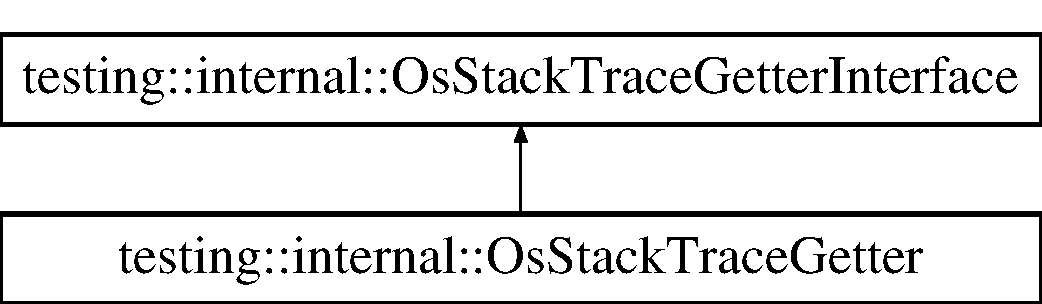
\includegraphics[height=2.000000cm]{classtesting_1_1internal_1_1OsStackTraceGetterInterface}
\end{center}
\end{figure}
\subsection*{Membros públicos}
\begin{DoxyCompactItemize}
\item 
\hypertarget{classtesting_1_1internal_1_1OsStackTraceGetterInterface_a6965eadb9b340808718fab9f1475c49a}{virtual string {\bfseries Current\-Stack\-Trace} (int max\-\_\-depth, int skip\-\_\-count)=0}\label{classtesting_1_1internal_1_1OsStackTraceGetterInterface_a6965eadb9b340808718fab9f1475c49a}

\item 
\hypertarget{classtesting_1_1internal_1_1OsStackTraceGetterInterface_a791bd120428b5a53d5eeba1b27296a39}{virtual void {\bfseries Upon\-Leaving\-G\-Test} ()=0}\label{classtesting_1_1internal_1_1OsStackTraceGetterInterface_a791bd120428b5a53d5eeba1b27296a39}

\end{DoxyCompactItemize}


A documentação para esta classe foi gerada a partir do seguinte ficheiro\-:\begin{DoxyCompactItemize}
\item 
src/gtest-\/internal-\/inl.\-h\end{DoxyCompactItemize}

\hypertarget{structPreRequisitos}{\section{Referência à estrutura Pre\-Requisitos}
\label{structPreRequisitos}\index{Pre\-Requisitos@{Pre\-Requisitos}}
}


{\ttfamily \#include $<$grafo.\-h$>$}

\subsection*{Atributos Públicos}
\begin{DoxyCompactItemize}
\item 
int \hyperlink{structPreRequisitos_aac895640418edfa91ba7c8f01b91459e}{id\-\_\-prerequisito}
\item 
struct \hyperlink{structPreRequisitos}{Pre\-Requisitos} $\ast$ \hyperlink{structPreRequisitos_ad30378886dd7fba5247ad1c77fb395f1}{prox}
\end{DoxyCompactItemize}


\subsection{Documentação dos dados membro}
\hypertarget{structPreRequisitos_aac895640418edfa91ba7c8f01b91459e}{\index{Pre\-Requisitos@{Pre\-Requisitos}!id\-\_\-prerequisito@{id\-\_\-prerequisito}}
\index{id\-\_\-prerequisito@{id\-\_\-prerequisito}!PreRequisitos@{Pre\-Requisitos}}
\subsubsection[{id\-\_\-prerequisito}]{\setlength{\rightskip}{0pt plus 5cm}int Pre\-Requisitos\-::id\-\_\-prerequisito}}\label{structPreRequisitos_aac895640418edfa91ba7c8f01b91459e}
\hypertarget{structPreRequisitos_ad30378886dd7fba5247ad1c77fb395f1}{\index{Pre\-Requisitos@{Pre\-Requisitos}!prox@{prox}}
\index{prox@{prox}!PreRequisitos@{Pre\-Requisitos}}
\subsubsection[{prox}]{\setlength{\rightskip}{0pt plus 5cm}struct {\bf Pre\-Requisitos}$\ast$ Pre\-Requisitos\-::prox}}\label{structPreRequisitos_ad30378886dd7fba5247ad1c77fb395f1}


A documentação para esta estrutura foi gerada a partir do seguinte ficheiro\-:\begin{DoxyCompactItemize}
\item 
code/\hyperlink{grafo_8h}{grafo.\-h}\end{DoxyCompactItemize}

\hypertarget{classtesting_1_1internal_1_1PrettyUnitTestResultPrinter}{\section{Referência à classe testing\-:\-:internal\-:\-:Pretty\-Unit\-Test\-Result\-Printer}
\label{classtesting_1_1internal_1_1PrettyUnitTestResultPrinter}\index{testing\-::internal\-::\-Pretty\-Unit\-Test\-Result\-Printer@{testing\-::internal\-::\-Pretty\-Unit\-Test\-Result\-Printer}}
}
Diagrama de heranças da classe testing\-:\-:internal\-:\-:Pretty\-Unit\-Test\-Result\-Printer\begin{figure}[H]
\begin{center}
\leavevmode
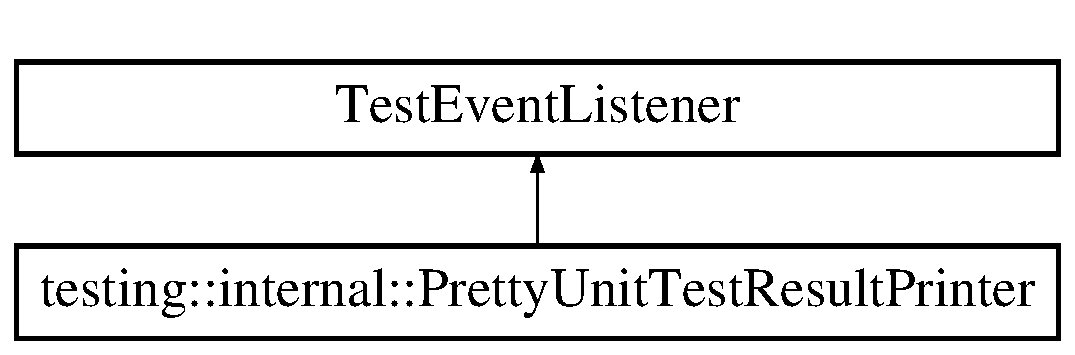
\includegraphics[height=2.000000cm]{classtesting_1_1internal_1_1PrettyUnitTestResultPrinter}
\end{center}
\end{figure}
\subsection*{Membros públicos}
\begin{DoxyCompactItemize}
\item 
\hypertarget{classtesting_1_1internal_1_1PrettyUnitTestResultPrinter_a7a6b6de195b4ef3c9f2edd2e6c270f3e}{virtual void {\bfseries On\-Test\-Program\-Start} (const \hyperlink{classtesting_1_1UnitTest}{Unit\-Test} \&)}\label{classtesting_1_1internal_1_1PrettyUnitTestResultPrinter_a7a6b6de195b4ef3c9f2edd2e6c270f3e}

\item 
\hypertarget{classtesting_1_1internal_1_1PrettyUnitTestResultPrinter_abdba10a8c97e272ab4cee97cb652c957}{virtual void {\bfseries On\-Test\-Iteration\-Start} (const \hyperlink{classtesting_1_1UnitTest}{Unit\-Test} \&unit\-\_\-test, int iteration)}\label{classtesting_1_1internal_1_1PrettyUnitTestResultPrinter_abdba10a8c97e272ab4cee97cb652c957}

\item 
\hypertarget{classtesting_1_1internal_1_1PrettyUnitTestResultPrinter_a846a5e82b421e04fcdd2b1b2b64b162f}{virtual void {\bfseries On\-Environments\-Set\-Up\-Start} (const \hyperlink{classtesting_1_1UnitTest}{Unit\-Test} \&unit\-\_\-test)}\label{classtesting_1_1internal_1_1PrettyUnitTestResultPrinter_a846a5e82b421e04fcdd2b1b2b64b162f}

\item 
\hypertarget{classtesting_1_1internal_1_1PrettyUnitTestResultPrinter_aadba892f02606a8b0c5f5982b3553aac}{virtual void {\bfseries On\-Environments\-Set\-Up\-End} (const \hyperlink{classtesting_1_1UnitTest}{Unit\-Test} \&)}\label{classtesting_1_1internal_1_1PrettyUnitTestResultPrinter_aadba892f02606a8b0c5f5982b3553aac}

\item 
\hypertarget{classtesting_1_1internal_1_1PrettyUnitTestResultPrinter_adcb68c729565d4bcdf8418a52902c3de}{virtual void {\bfseries On\-Test\-Case\-Start} (const \hyperlink{classtesting_1_1TestCase}{Test\-Case} \&test\-\_\-case)}\label{classtesting_1_1internal_1_1PrettyUnitTestResultPrinter_adcb68c729565d4bcdf8418a52902c3de}

\item 
\hypertarget{classtesting_1_1internal_1_1PrettyUnitTestResultPrinter_a5078ee71cfa97e37ae7a9366149195c5}{virtual void {\bfseries On\-Test\-Start} (const \hyperlink{classtesting_1_1TestInfo}{Test\-Info} \&test\-\_\-info)}\label{classtesting_1_1internal_1_1PrettyUnitTestResultPrinter_a5078ee71cfa97e37ae7a9366149195c5}

\item 
\hypertarget{classtesting_1_1internal_1_1PrettyUnitTestResultPrinter_a7589e8df7485349498a3a81bf16e2f68}{virtual void {\bfseries On\-Test\-Part\-Result} (const \hyperlink{classtesting_1_1TestPartResult}{Test\-Part\-Result} \&result)}\label{classtesting_1_1internal_1_1PrettyUnitTestResultPrinter_a7589e8df7485349498a3a81bf16e2f68}

\item 
\hypertarget{classtesting_1_1internal_1_1PrettyUnitTestResultPrinter_a06749ff2b32a16c127374ecd015f13e0}{virtual void {\bfseries On\-Test\-End} (const \hyperlink{classtesting_1_1TestInfo}{Test\-Info} \&test\-\_\-info)}\label{classtesting_1_1internal_1_1PrettyUnitTestResultPrinter_a06749ff2b32a16c127374ecd015f13e0}

\item 
\hypertarget{classtesting_1_1internal_1_1PrettyUnitTestResultPrinter_a7a62fe58fa6f6aace813eb62b31e5a51}{virtual void {\bfseries On\-Test\-Case\-End} (const \hyperlink{classtesting_1_1TestCase}{Test\-Case} \&test\-\_\-case)}\label{classtesting_1_1internal_1_1PrettyUnitTestResultPrinter_a7a62fe58fa6f6aace813eb62b31e5a51}

\item 
\hypertarget{classtesting_1_1internal_1_1PrettyUnitTestResultPrinter_afea9dc849c92fdbc1d8505f4c74ffc1a}{virtual void {\bfseries On\-Environments\-Tear\-Down\-Start} (const \hyperlink{classtesting_1_1UnitTest}{Unit\-Test} \&unit\-\_\-test)}\label{classtesting_1_1internal_1_1PrettyUnitTestResultPrinter_afea9dc849c92fdbc1d8505f4c74ffc1a}

\item 
\hypertarget{classtesting_1_1internal_1_1PrettyUnitTestResultPrinter_ab23094ef3b714778b2f742d39818c280}{virtual void {\bfseries On\-Environments\-Tear\-Down\-End} (const \hyperlink{classtesting_1_1UnitTest}{Unit\-Test} \&)}\label{classtesting_1_1internal_1_1PrettyUnitTestResultPrinter_ab23094ef3b714778b2f742d39818c280}

\item 
\hypertarget{classtesting_1_1internal_1_1PrettyUnitTestResultPrinter_ac29b30216023baddda04ef5889f484ff}{virtual void {\bfseries On\-Test\-Iteration\-End} (const \hyperlink{classtesting_1_1UnitTest}{Unit\-Test} \&unit\-\_\-test, int iteration)}\label{classtesting_1_1internal_1_1PrettyUnitTestResultPrinter_ac29b30216023baddda04ef5889f484ff}

\item 
\hypertarget{classtesting_1_1internal_1_1PrettyUnitTestResultPrinter_a8c92c062889abdb940b04ffe113f5980}{virtual void {\bfseries On\-Test\-Program\-End} (const \hyperlink{classtesting_1_1UnitTest}{Unit\-Test} \&)}\label{classtesting_1_1internal_1_1PrettyUnitTestResultPrinter_a8c92c062889abdb940b04ffe113f5980}

\end{DoxyCompactItemize}
\subsection*{Membros públicos estáticos}
\begin{DoxyCompactItemize}
\item 
\hypertarget{classtesting_1_1internal_1_1PrettyUnitTestResultPrinter_a5b60a9aed1db02837b11450f6e8d0f71}{static void {\bfseries Print\-Test\-Name} (const char $\ast$test\-\_\-case, const char $\ast$test)}\label{classtesting_1_1internal_1_1PrettyUnitTestResultPrinter_a5b60a9aed1db02837b11450f6e8d0f71}

\end{DoxyCompactItemize}


A documentação para esta classe foi gerada a partir do seguinte ficheiro\-:\begin{DoxyCompactItemize}
\item 
src/gtest.\-cc\end{DoxyCompactItemize}

\hypertarget{classtesting_1_1internal_1_1Random}{\section{Referência à classe testing\-:\-:internal\-:\-:Random}
\label{classtesting_1_1internal_1_1Random}\index{testing\-::internal\-::\-Random@{testing\-::internal\-::\-Random}}
}
\subsection*{Membros públicos}
\begin{DoxyCompactItemize}
\item 
\hypertarget{classtesting_1_1internal_1_1Random_a6e112be5e7cce00551f6383025f69460}{{\bfseries Random} (U\-Int32 seed)}\label{classtesting_1_1internal_1_1Random_a6e112be5e7cce00551f6383025f69460}

\item 
\hypertarget{classtesting_1_1internal_1_1Random_adf2f24199318a46f885c78f50d89a69e}{void {\bfseries Reseed} (U\-Int32 seed)}\label{classtesting_1_1internal_1_1Random_adf2f24199318a46f885c78f50d89a69e}

\item 
\hypertarget{classtesting_1_1internal_1_1Random_a9315b7fb621cbcfdf92ed4b5e584c0db}{U\-Int32 {\bfseries Generate} (U\-Int32 range)}\label{classtesting_1_1internal_1_1Random_a9315b7fb621cbcfdf92ed4b5e584c0db}

\end{DoxyCompactItemize}
\subsection*{Atributos Públicos Estáticos}
\begin{DoxyCompactItemize}
\item 
\hypertarget{classtesting_1_1internal_1_1Random_a36d72dd7063d0b5338f229e75382fdd2}{static const U\-Int32 {\bfseries k\-Max\-Range} = 1u $<$$<$ 31}\label{classtesting_1_1internal_1_1Random_a36d72dd7063d0b5338f229e75382fdd2}

\end{DoxyCompactItemize}


A documentação para esta classe foi gerada a partir dos seguintes ficheiros\-:\begin{DoxyCompactItemize}
\item 
include/gtest/internal/gtest-\/internal.\-h\item 
src/gtest.\-cc\end{DoxyCompactItemize}

\hypertarget{classtesting_1_1internal_1_1RE}{\section{Referência à classe testing\-:\-:internal\-:\-:R\-E}
\label{classtesting_1_1internal_1_1RE}\index{testing\-::internal\-::\-R\-E@{testing\-::internal\-::\-R\-E}}
}
\subsection*{Membros públicos}
\begin{DoxyCompactItemize}
\item 
\hypertarget{classtesting_1_1internal_1_1RE_ab215dbc2565fce641e1746ca43e9d68a}{{\bfseries R\-E} (const \hyperlink{classtesting_1_1internal_1_1RE}{R\-E} \&other)}\label{classtesting_1_1internal_1_1RE_ab215dbc2565fce641e1746ca43e9d68a}

\item 
\hypertarget{classtesting_1_1internal_1_1RE_a8840bd639642f3d4769a94a68ce463c2}{{\bfseries R\-E} (const \-::std\-::string \&regex)}\label{classtesting_1_1internal_1_1RE_a8840bd639642f3d4769a94a68ce463c2}

\item 
\hypertarget{classtesting_1_1internal_1_1RE_a908ea936a5b7a14479a1b292a7189ca6}{{\bfseries R\-E} (const char $\ast$regex)}\label{classtesting_1_1internal_1_1RE_a908ea936a5b7a14479a1b292a7189ca6}

\item 
\hypertarget{classtesting_1_1internal_1_1RE_acb67d77f53e73af81cce6dcd663c94df}{const char $\ast$ {\bfseries pattern} () const }\label{classtesting_1_1internal_1_1RE_acb67d77f53e73af81cce6dcd663c94df}

\end{DoxyCompactItemize}
\subsection*{Membros públicos estáticos}
\begin{DoxyCompactItemize}
\item 
\hypertarget{classtesting_1_1internal_1_1RE_aa79a950758d0f1d62f7762d1e9cefe86}{static bool {\bfseries Full\-Match} (const \-::std\-::string \&str, const \hyperlink{classtesting_1_1internal_1_1RE}{R\-E} \&re)}\label{classtesting_1_1internal_1_1RE_aa79a950758d0f1d62f7762d1e9cefe86}

\item 
\hypertarget{classtesting_1_1internal_1_1RE_a1e81f9a87211bdca645e025f8f0236c8}{static bool {\bfseries Partial\-Match} (const \-::std\-::string \&str, const \hyperlink{classtesting_1_1internal_1_1RE}{R\-E} \&re)}\label{classtesting_1_1internal_1_1RE_a1e81f9a87211bdca645e025f8f0236c8}

\item 
\hypertarget{classtesting_1_1internal_1_1RE_a2b13ec1f6ccd6c32f7efa01e21588f0b}{static bool {\bfseries Full\-Match} (const char $\ast$str, const \hyperlink{classtesting_1_1internal_1_1RE}{R\-E} \&re)}\label{classtesting_1_1internal_1_1RE_a2b13ec1f6ccd6c32f7efa01e21588f0b}

\item 
\hypertarget{classtesting_1_1internal_1_1RE_a97495dd4c2bb9589522823f060c8e8ba}{static bool {\bfseries Partial\-Match} (const char $\ast$str, const \hyperlink{classtesting_1_1internal_1_1RE}{R\-E} \&re)}\label{classtesting_1_1internal_1_1RE_a97495dd4c2bb9589522823f060c8e8ba}

\end{DoxyCompactItemize}


A documentação para esta classe foi gerada a partir do seguinte ficheiro\-:\begin{DoxyCompactItemize}
\item 
include/gtest/internal/gtest-\/port.\-h\end{DoxyCompactItemize}

\hypertarget{structtesting_1_1internal_1_1RemoveConst}{\section{Referência à estrutura Template testing\-:\-:internal\-:\-:Remove\-Const$<$ T $>$}
\label{structtesting_1_1internal_1_1RemoveConst}\index{testing\-::internal\-::\-Remove\-Const$<$ T $>$@{testing\-::internal\-::\-Remove\-Const$<$ T $>$}}
}
\subsection*{Tipos Públicos}
\begin{DoxyCompactItemize}
\item 
\hypertarget{structtesting_1_1internal_1_1RemoveConst_a1be32027ea4edcc0d15abd59aba4a97f}{typedef T {\bfseries type}}\label{structtesting_1_1internal_1_1RemoveConst_a1be32027ea4edcc0d15abd59aba4a97f}

\end{DoxyCompactItemize}


A documentação para esta estrutura foi gerada a partir do seguinte ficheiro\-:\begin{DoxyCompactItemize}
\item 
include/gtest/internal/gtest-\/internal.\-h\end{DoxyCompactItemize}

\hypertarget{structtesting_1_1internal_1_1RemoveConst_3_01const_01T_01_4}{\section{Referência à estrutura Template testing\-:\-:internal\-:\-:Remove\-Const$<$ const T $>$}
\label{structtesting_1_1internal_1_1RemoveConst_3_01const_01T_01_4}\index{testing\-::internal\-::\-Remove\-Const$<$ const T $>$@{testing\-::internal\-::\-Remove\-Const$<$ const T $>$}}
}
\subsection*{Tipos Públicos}
\begin{DoxyCompactItemize}
\item 
\hypertarget{structtesting_1_1internal_1_1RemoveConst_3_01const_01T_01_4_ac88c6824d228ab05091e5a4f1c1a95fc}{typedef T {\bfseries type}}\label{structtesting_1_1internal_1_1RemoveConst_3_01const_01T_01_4_ac88c6824d228ab05091e5a4f1c1a95fc}

\end{DoxyCompactItemize}


A documentação para esta estrutura foi gerada a partir do seguinte ficheiro\-:\begin{DoxyCompactItemize}
\item 
include/gtest/internal/gtest-\/internal.\-h\end{DoxyCompactItemize}

\hypertarget{structtesting_1_1internal_1_1RemoveConst_3_01const_01T[N]_4}{\section{Referência à estrutura Template testing\-:\-:internal\-:\-:Remove\-Const$<$ const T\mbox{[}N\mbox{]}$>$}
\label{structtesting_1_1internal_1_1RemoveConst_3_01const_01T[N]_4}\index{testing\-::internal\-::\-Remove\-Const$<$ const T\mbox{[}\-N\mbox{]}$>$@{testing\-::internal\-::\-Remove\-Const$<$ const T[N]$>$}}
}
\subsection*{Tipos Públicos}
\begin{DoxyCompactItemize}
\item 
\hypertarget{structtesting_1_1internal_1_1RemoveConst_3_01const_01T[N]_4_ac976b53cb5d031a120fafbe790650068}{typedef \hyperlink{structtesting_1_1internal_1_1RemoveConst}{Remove\-Const}$<$ T $>$\-::type {\bfseries type} \mbox{[}N\mbox{]}}\label{structtesting_1_1internal_1_1RemoveConst_3_01const_01T[N]_4_ac976b53cb5d031a120fafbe790650068}

\end{DoxyCompactItemize}


A documentação para esta estrutura foi gerada a partir do seguinte ficheiro\-:\begin{DoxyCompactItemize}
\item 
include/gtest/internal/gtest-\/internal.\-h\end{DoxyCompactItemize}

\hypertarget{structtesting_1_1internal_1_1RemoveReference}{\section{Referência à estrutura Template testing\-:\-:internal\-:\-:Remove\-Reference$<$ T $>$}
\label{structtesting_1_1internal_1_1RemoveReference}\index{testing\-::internal\-::\-Remove\-Reference$<$ T $>$@{testing\-::internal\-::\-Remove\-Reference$<$ T $>$}}
}
\subsection*{Tipos Públicos}
\begin{DoxyCompactItemize}
\item 
\hypertarget{structtesting_1_1internal_1_1RemoveReference_a9ca4f6499579225f7986b789ee4b2895}{typedef T {\bfseries type}}\label{structtesting_1_1internal_1_1RemoveReference_a9ca4f6499579225f7986b789ee4b2895}

\end{DoxyCompactItemize}


A documentação para esta estrutura foi gerada a partir do seguinte ficheiro\-:\begin{DoxyCompactItemize}
\item 
include/gtest/internal/gtest-\/internal.\-h\end{DoxyCompactItemize}

\hypertarget{structtesting_1_1internal_1_1RemoveReference_3_01T_01_6_01_4}{\section{Referência à estrutura Template testing\-:\-:internal\-:\-:Remove\-Reference$<$ T \& $>$}
\label{structtesting_1_1internal_1_1RemoveReference_3_01T_01_6_01_4}\index{testing\-::internal\-::\-Remove\-Reference$<$ T \& $>$@{testing\-::internal\-::\-Remove\-Reference$<$ T \& $>$}}
}
\subsection*{Tipos Públicos}
\begin{DoxyCompactItemize}
\item 
\hypertarget{structtesting_1_1internal_1_1RemoveReference_3_01T_01_6_01_4_a3d0f32a66759f333c2dd66aa31005e6d}{typedef T {\bfseries type}}\label{structtesting_1_1internal_1_1RemoveReference_3_01T_01_6_01_4_a3d0f32a66759f333c2dd66aa31005e6d}

\end{DoxyCompactItemize}


A documentação para esta estrutura foi gerada a partir do seguinte ficheiro\-:\begin{DoxyCompactItemize}
\item 
include/gtest/internal/gtest-\/internal.\-h\end{DoxyCompactItemize}

\hypertarget{structstd_1_1tr1_1_1gtest__internal_1_1SameSizeTuplePrefixComparator}{\section{Referência à estrutura Template std\-:\-:tr1\-:\-:gtest\-\_\-internal\-:\-:Same\-Size\-Tuple\-Prefix\-Comparator$<$ k\-Size1, k\-Size2 $>$}
\label{structstd_1_1tr1_1_1gtest__internal_1_1SameSizeTuplePrefixComparator}\index{std\-::tr1\-::gtest\-\_\-internal\-::\-Same\-Size\-Tuple\-Prefix\-Comparator$<$ k\-Size1, k\-Size2 $>$@{std\-::tr1\-::gtest\-\_\-internal\-::\-Same\-Size\-Tuple\-Prefix\-Comparator$<$ k\-Size1, k\-Size2 $>$}}
}


A documentação para esta estrutura foi gerada a partir do seguinte ficheiro\-:\begin{DoxyCompactItemize}
\item 
include/gtest/internal/gtest-\/tuple.\-h\end{DoxyCompactItemize}

\hypertarget{structstd_1_1tr1_1_1gtest__internal_1_1SameSizeTuplePrefixComparator_3_010_00_010_01_4}{\section{Referência à estrutura Template std\-:\-:tr1\-:\-:gtest\-\_\-internal\-:\-:Same\-Size\-Tuple\-Prefix\-Comparator$<$ 0, 0 $>$}
\label{structstd_1_1tr1_1_1gtest__internal_1_1SameSizeTuplePrefixComparator_3_010_00_010_01_4}\index{std\-::tr1\-::gtest\-\_\-internal\-::\-Same\-Size\-Tuple\-Prefix\-Comparator$<$ 0, 0 $>$@{std\-::tr1\-::gtest\-\_\-internal\-::\-Same\-Size\-Tuple\-Prefix\-Comparator$<$ 0, 0 $>$}}
}
\subsection*{Membros públicos estáticos}
\begin{DoxyCompactItemize}
\item 
\hypertarget{structstd_1_1tr1_1_1gtest__internal_1_1SameSizeTuplePrefixComparator_3_010_00_010_01_4_a4f209822266c6bb1832c49750a11ef95}{{\footnotesize template$<$class Tuple1 , class Tuple2 $>$ }\\static bool {\bfseries Eq} (const Tuple1 \&, const Tuple2 \&)}\label{structstd_1_1tr1_1_1gtest__internal_1_1SameSizeTuplePrefixComparator_3_010_00_010_01_4_a4f209822266c6bb1832c49750a11ef95}

\end{DoxyCompactItemize}


A documentação para esta estrutura foi gerada a partir do seguinte ficheiro\-:\begin{DoxyCompactItemize}
\item 
include/gtest/internal/gtest-\/tuple.\-h\end{DoxyCompactItemize}

\hypertarget{structstd_1_1tr1_1_1gtest__internal_1_1SameSizeTuplePrefixComparator_3_01k_00_01k_01_4}{\section{Referência à estrutura Template std\-:\-:tr1\-:\-:gtest\-\_\-internal\-:\-:Same\-Size\-Tuple\-Prefix\-Comparator$<$ k, k $>$}
\label{structstd_1_1tr1_1_1gtest__internal_1_1SameSizeTuplePrefixComparator_3_01k_00_01k_01_4}\index{std\-::tr1\-::gtest\-\_\-internal\-::\-Same\-Size\-Tuple\-Prefix\-Comparator$<$ k, k $>$@{std\-::tr1\-::gtest\-\_\-internal\-::\-Same\-Size\-Tuple\-Prefix\-Comparator$<$ k, k $>$}}
}
\subsection*{Membros públicos estáticos}
\begin{DoxyCompactItemize}
\item 
\hypertarget{structstd_1_1tr1_1_1gtest__internal_1_1SameSizeTuplePrefixComparator_3_01k_00_01k_01_4_a5564fbade05a2d0522d9899da62c2119}{{\footnotesize template$<$class Tuple1 , class Tuple2 $>$ }\\static bool {\bfseries Eq} (const Tuple1 \&t1, const Tuple2 \&t2)}\label{structstd_1_1tr1_1_1gtest__internal_1_1SameSizeTuplePrefixComparator_3_01k_00_01k_01_4_a5564fbade05a2d0522d9899da62c2119}

\end{DoxyCompactItemize}


A documentação para esta estrutura foi gerada a partir do seguinte ficheiro\-:\begin{DoxyCompactItemize}
\item 
include/gtest/internal/gtest-\/tuple.\-h\end{DoxyCompactItemize}

\hypertarget{classtesting_1_1internal_1_1scoped__ptr}{\section{Referência à classe Template testing\-:\-:internal\-:\-:scoped\-\_\-ptr$<$ T $>$}
\label{classtesting_1_1internal_1_1scoped__ptr}\index{testing\-::internal\-::scoped\-\_\-ptr$<$ T $>$@{testing\-::internal\-::scoped\-\_\-ptr$<$ T $>$}}
}
\subsection*{Tipos Públicos}
\begin{DoxyCompactItemize}
\item 
\hypertarget{classtesting_1_1internal_1_1scoped__ptr_ae755ffeebada8e20b68c1d1ffa91cf13}{typedef T {\bfseries element\-\_\-type}}\label{classtesting_1_1internal_1_1scoped__ptr_ae755ffeebada8e20b68c1d1ffa91cf13}

\end{DoxyCompactItemize}
\subsection*{Membros públicos}
\begin{DoxyCompactItemize}
\item 
\hypertarget{classtesting_1_1internal_1_1scoped__ptr_adb972432999a0c63720df148964ac2a5}{{\bfseries scoped\-\_\-ptr} (T $\ast$p=N\-U\-L\-L)}\label{classtesting_1_1internal_1_1scoped__ptr_adb972432999a0c63720df148964ac2a5}

\item 
\hypertarget{classtesting_1_1internal_1_1scoped__ptr_ab197837f87062de69d9d6e04539bbabe}{T \& {\bfseries operator$\ast$} () const }\label{classtesting_1_1internal_1_1scoped__ptr_ab197837f87062de69d9d6e04539bbabe}

\item 
\hypertarget{classtesting_1_1internal_1_1scoped__ptr_adc38310fbbe400faf9279e36000a17c4}{T $\ast$ {\bfseries operator-\/$>$} () const }\label{classtesting_1_1internal_1_1scoped__ptr_adc38310fbbe400faf9279e36000a17c4}

\item 
\hypertarget{classtesting_1_1internal_1_1scoped__ptr_adc8f8fcb63ce69f80f011456e6d2f08d}{T $\ast$ {\bfseries get} () const }\label{classtesting_1_1internal_1_1scoped__ptr_adc8f8fcb63ce69f80f011456e6d2f08d}

\item 
\hypertarget{classtesting_1_1internal_1_1scoped__ptr_a7a4f3e568d81a5d8bcb5f8d6bf5130b1}{T $\ast$ {\bfseries release} ()}\label{classtesting_1_1internal_1_1scoped__ptr_a7a4f3e568d81a5d8bcb5f8d6bf5130b1}

\item 
\hypertarget{classtesting_1_1internal_1_1scoped__ptr_acac03266a43359801aff0de5c990bec0}{void {\bfseries reset} (T $\ast$p=N\-U\-L\-L)}\label{classtesting_1_1internal_1_1scoped__ptr_acac03266a43359801aff0de5c990bec0}

\end{DoxyCompactItemize}


A documentação para esta classe foi gerada a partir do seguinte ficheiro\-:\begin{DoxyCompactItemize}
\item 
include/gtest/internal/gtest-\/port.\-h\end{DoxyCompactItemize}

\hypertarget{classtesting_1_1ScopedFakeTestPartResultReporter}{\section{Referência à classe testing\-:\-:Scoped\-Fake\-Test\-Part\-Result\-Reporter}
\label{classtesting_1_1ScopedFakeTestPartResultReporter}\index{testing\-::\-Scoped\-Fake\-Test\-Part\-Result\-Reporter@{testing\-::\-Scoped\-Fake\-Test\-Part\-Result\-Reporter}}
}
Diagrama de heranças da classe testing\-:\-:Scoped\-Fake\-Test\-Part\-Result\-Reporter\begin{figure}[H]
\begin{center}
\leavevmode
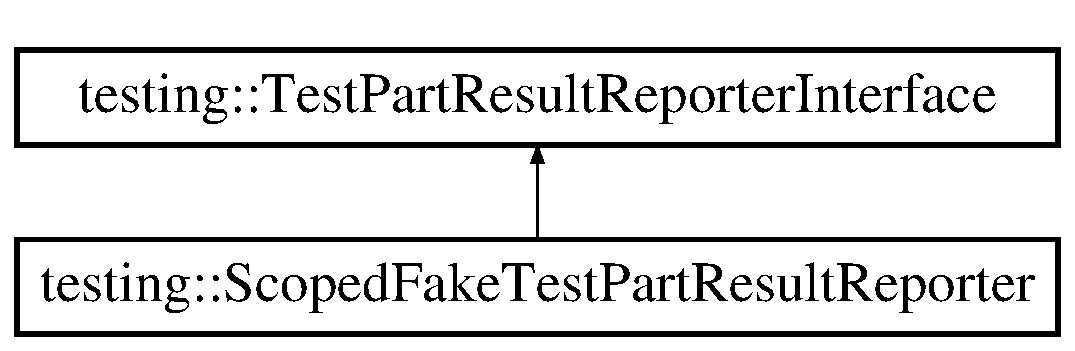
\includegraphics[height=2.000000cm]{classtesting_1_1ScopedFakeTestPartResultReporter}
\end{center}
\end{figure}
\subsection*{Tipos Públicos}
\begin{DoxyCompactItemize}
\item 
enum {\bfseries Intercept\-Mode} \{ {\bfseries I\-N\-T\-E\-R\-C\-E\-P\-T\-\_\-\-O\-N\-L\-Y\-\_\-\-C\-U\-R\-R\-E\-N\-T\-\_\-\-T\-H\-R\-E\-A\-D}, 
{\bfseries I\-N\-T\-E\-R\-C\-E\-P\-T\-\_\-\-A\-L\-L\-\_\-\-T\-H\-R\-E\-A\-D\-S}
 \}
\end{DoxyCompactItemize}
\subsection*{Membros públicos}
\begin{DoxyCompactItemize}
\item 
\hypertarget{classtesting_1_1ScopedFakeTestPartResultReporter_aa0100ecf4799fb51d45167be6a5de1d5}{{\bfseries Scoped\-Fake\-Test\-Part\-Result\-Reporter} (\hyperlink{classtesting_1_1TestPartResultArray}{Test\-Part\-Result\-Array} $\ast$result)}\label{classtesting_1_1ScopedFakeTestPartResultReporter_aa0100ecf4799fb51d45167be6a5de1d5}

\item 
\hypertarget{classtesting_1_1ScopedFakeTestPartResultReporter_a57cbc09ed48627c8a73e622618dc4b4f}{{\bfseries Scoped\-Fake\-Test\-Part\-Result\-Reporter} (Intercept\-Mode intercept\-\_\-mode, \hyperlink{classtesting_1_1TestPartResultArray}{Test\-Part\-Result\-Array} $\ast$result)}\label{classtesting_1_1ScopedFakeTestPartResultReporter_a57cbc09ed48627c8a73e622618dc4b4f}

\item 
\hypertarget{classtesting_1_1ScopedFakeTestPartResultReporter_a82531434f51632d98ed7cdcdb10b8b92}{virtual void {\bfseries Report\-Test\-Part\-Result} (const \hyperlink{classtesting_1_1TestPartResult}{Test\-Part\-Result} \&result)}\label{classtesting_1_1ScopedFakeTestPartResultReporter_a82531434f51632d98ed7cdcdb10b8b92}

\end{DoxyCompactItemize}


A documentação para esta classe foi gerada a partir dos seguintes ficheiros\-:\begin{DoxyCompactItemize}
\item 
include/gtest/gtest-\/spi.\-h\item 
src/gtest.\-cc\end{DoxyCompactItemize}

\hypertarget{classtesting_1_1internal_1_1ScopedPrematureExitFile}{\section{Referência à classe testing\-:\-:internal\-:\-:Scoped\-Premature\-Exit\-File}
\label{classtesting_1_1internal_1_1ScopedPrematureExitFile}\index{testing\-::internal\-::\-Scoped\-Premature\-Exit\-File@{testing\-::internal\-::\-Scoped\-Premature\-Exit\-File}}
}
\subsection*{Membros públicos}
\begin{DoxyCompactItemize}
\item 
\hypertarget{classtesting_1_1internal_1_1ScopedPrematureExitFile_ae520883b8a6984a864ce675acedff4a2}{{\bfseries Scoped\-Premature\-Exit\-File} (const char $\ast$premature\-\_\-exit\-\_\-filepath)}\label{classtesting_1_1internal_1_1ScopedPrematureExitFile_ae520883b8a6984a864ce675acedff4a2}

\end{DoxyCompactItemize}


A documentação para esta classe foi gerada a partir do seguinte ficheiro\-:\begin{DoxyCompactItemize}
\item 
src/gtest.\-cc\end{DoxyCompactItemize}

\hypertarget{classtesting_1_1internal_1_1ScopedTrace}{\section{Referência à classe testing\-:\-:internal\-:\-:Scoped\-Trace}
\label{classtesting_1_1internal_1_1ScopedTrace}\index{testing\-::internal\-::\-Scoped\-Trace@{testing\-::internal\-::\-Scoped\-Trace}}
}
\subsection*{Membros públicos}
\begin{DoxyCompactItemize}
\item 
\hypertarget{classtesting_1_1internal_1_1ScopedTrace_ab965d7010bbbc82c1bef6ebf8748bede}{{\bfseries Scoped\-Trace} (const char $\ast$file, int line, const \hyperlink{classtesting_1_1Message}{Message} \&message)}\label{classtesting_1_1internal_1_1ScopedTrace_ab965d7010bbbc82c1bef6ebf8748bede}

\end{DoxyCompactItemize}


A documentação para esta classe foi gerada a partir dos seguintes ficheiros\-:\begin{DoxyCompactItemize}
\item 
include/gtest/internal/gtest-\/internal.\-h\item 
src/gtest.\-cc\end{DoxyCompactItemize}

\hypertarget{classtesting_1_1internal_1_1SingleFailureChecker}{\section{Referência à classe testing\-:\-:internal\-:\-:Single\-Failure\-Checker}
\label{classtesting_1_1internal_1_1SingleFailureChecker}\index{testing\-::internal\-::\-Single\-Failure\-Checker@{testing\-::internal\-::\-Single\-Failure\-Checker}}
}
\subsection*{Membros públicos}
\begin{DoxyCompactItemize}
\item 
\hypertarget{classtesting_1_1internal_1_1SingleFailureChecker_a6d350d385526c97c9982e928f5f8fb56}{{\bfseries Single\-Failure\-Checker} (const \hyperlink{classtesting_1_1TestPartResultArray}{Test\-Part\-Result\-Array} $\ast$results, Test\-Part\-Result\-::\-Type type, const string \&substr)}\label{classtesting_1_1internal_1_1SingleFailureChecker_a6d350d385526c97c9982e928f5f8fb56}

\end{DoxyCompactItemize}


A documentação para esta classe foi gerada a partir dos seguintes ficheiros\-:\begin{DoxyCompactItemize}
\item 
include/gtest/gtest-\/spi.\-h\item 
src/gtest.\-cc\end{DoxyCompactItemize}

\hypertarget{structtesting_1_1internal_1_1StaticAssertTypeEqHelper}{\section{Referência à estrutura Template testing\-:\-:internal\-:\-:Static\-Assert\-Type\-Eq\-Helper$<$ T1, T2 $>$}
\label{structtesting_1_1internal_1_1StaticAssertTypeEqHelper}\index{testing\-::internal\-::\-Static\-Assert\-Type\-Eq\-Helper$<$ T1, T2 $>$@{testing\-::internal\-::\-Static\-Assert\-Type\-Eq\-Helper$<$ T1, T2 $>$}}
}


A documentação para esta estrutura foi gerada a partir do seguinte ficheiro\-:\begin{DoxyCompactItemize}
\item 
include/gtest/internal/gtest-\/port.\-h\end{DoxyCompactItemize}

\hypertarget{structtesting_1_1internal_1_1StaticAssertTypeEqHelper_3_01T_00_01T_01_4}{\section{Referência à estrutura Template testing\-:\-:internal\-:\-:Static\-Assert\-Type\-Eq\-Helper$<$ T, T $>$}
\label{structtesting_1_1internal_1_1StaticAssertTypeEqHelper_3_01T_00_01T_01_4}\index{testing\-::internal\-::\-Static\-Assert\-Type\-Eq\-Helper$<$ T, T $>$@{testing\-::internal\-::\-Static\-Assert\-Type\-Eq\-Helper$<$ T, T $>$}}
}


A documentação para esta estrutura foi gerada a partir do seguinte ficheiro\-:\begin{DoxyCompactItemize}
\item 
include/gtest/internal/gtest-\/port.\-h\end{DoxyCompactItemize}

\hypertarget{classtesting_1_1internal_1_1String}{\section{Referência à classe testing\-:\-:internal\-:\-:String}
\label{classtesting_1_1internal_1_1String}\index{testing\-::internal\-::\-String@{testing\-::internal\-::\-String}}
}
\subsection*{Membros públicos estáticos}
\begin{DoxyCompactItemize}
\item 
\hypertarget{classtesting_1_1internal_1_1String_a8bce6b1281ae3d2f9061b920aa78aca0}{static const char $\ast$ {\bfseries Clone\-C\-String} (const char $\ast$c\-\_\-str)}\label{classtesting_1_1internal_1_1String_a8bce6b1281ae3d2f9061b920aa78aca0}

\item 
\hypertarget{classtesting_1_1internal_1_1String_a8bea7b33e7effbd299a0b4a5522ea96e}{static bool {\bfseries C\-String\-Equals} (const char $\ast$lhs, const char $\ast$rhs)}\label{classtesting_1_1internal_1_1String_a8bea7b33e7effbd299a0b4a5522ea96e}

\item 
\hypertarget{classtesting_1_1internal_1_1String_aaf7e376ff580677ea4954d5913d5b917}{static std\-::string {\bfseries Show\-Wide\-C\-String} (const wchar\-\_\-t $\ast$wide\-\_\-c\-\_\-str)}\label{classtesting_1_1internal_1_1String_aaf7e376ff580677ea4954d5913d5b917}

\item 
\hypertarget{classtesting_1_1internal_1_1String_ab0373bf6e96453d6ca0de2e68df13d3a}{static bool {\bfseries Wide\-C\-String\-Equals} (const wchar\-\_\-t $\ast$lhs, const wchar\-\_\-t $\ast$rhs)}\label{classtesting_1_1internal_1_1String_ab0373bf6e96453d6ca0de2e68df13d3a}

\item 
\hypertarget{classtesting_1_1internal_1_1String_a116ca435d63306927ba19f90a3596787}{static bool {\bfseries Case\-Insensitive\-C\-String\-Equals} (const char $\ast$lhs, const char $\ast$rhs)}\label{classtesting_1_1internal_1_1String_a116ca435d63306927ba19f90a3596787}

\item 
\hypertarget{classtesting_1_1internal_1_1String_a1f12d1780ca7afbf8975f5d425b9f362}{static bool {\bfseries Case\-Insensitive\-Wide\-C\-String\-Equals} (const wchar\-\_\-t $\ast$lhs, const wchar\-\_\-t $\ast$rhs)}\label{classtesting_1_1internal_1_1String_a1f12d1780ca7afbf8975f5d425b9f362}

\item 
\hypertarget{classtesting_1_1internal_1_1String_a968f242b709f8c7c0ed5ecf246553321}{static bool {\bfseries Ends\-With\-Case\-Insensitive} (const std\-::string \&str, const std\-::string \&suffix)}\label{classtesting_1_1internal_1_1String_a968f242b709f8c7c0ed5ecf246553321}

\item 
\hypertarget{classtesting_1_1internal_1_1String_af50b18d588355871e1982c4043523e0f}{static std\-::string {\bfseries Format\-Int\-Width2} (int value)}\label{classtesting_1_1internal_1_1String_af50b18d588355871e1982c4043523e0f}

\item 
\hypertarget{classtesting_1_1internal_1_1String_affe59102e49092fc0684388e9b0c5c1e}{static std\-::string {\bfseries Format\-Hex\-Int} (int value)}\label{classtesting_1_1internal_1_1String_affe59102e49092fc0684388e9b0c5c1e}

\item 
\hypertarget{classtesting_1_1internal_1_1String_af702dc7cbd569589d8e3ff215a7cafa9}{static std\-::string {\bfseries Format\-Byte} (unsigned char value)}\label{classtesting_1_1internal_1_1String_af702dc7cbd569589d8e3ff215a7cafa9}

\end{DoxyCompactItemize}


A documentação para esta classe foi gerada a partir dos seguintes ficheiros\-:\begin{DoxyCompactItemize}
\item 
include/gtest/internal/gtest-\/string.\-h\item 
src/gtest.\-cc\end{DoxyCompactItemize}

\hypertarget{structTarefa}{\section{Referência à estrutura Tarefa}
\label{structTarefa}\index{Tarefa@{Tarefa}}
}


{\ttfamily \#include $<$grafo.\-h$>$}



Diagrama de colaboração para Tarefa\-:
\nopagebreak
\begin{figure}[H]
\begin{center}
\leavevmode
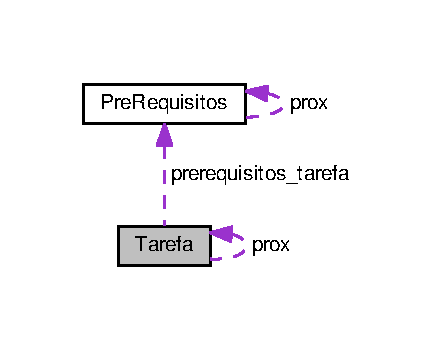
\includegraphics[width=208pt]{structTarefa__coll__graph}
\end{center}
\end{figure}
\subsection*{Atributos Públicos}
\begin{DoxyCompactItemize}
\item 
int \hyperlink{structTarefa_a1509b75b75f758e2d0502df4162366f2}{id\-\_\-tarefa}
\item 
char \hyperlink{structTarefa_a43c0db59f4e6a3031ef2a5951ad8910f}{nome\-\_\-tarefa} \mbox{[}\hyperlink{grafo_8h_a5d28dfdab86222715d699097e8cd092f}{T\-A\-M\-\_\-\-S\-T\-R\-I\-N\-G}\mbox{]}
\item 
int \hyperlink{structTarefa_a86ef331b855e3f91eec492a00171cc9c}{tarefa\-\_\-executada}
\item 
int \hyperlink{structTarefa_a7962bef326f487f4ffa7dc0f04153729}{duracao\-\_\-tarefa}
\item 
int \hyperlink{structTarefa_a7d09c30d0162c55a0aab1ad71716fae6}{inicio\-\_\-min\-\_\-tarefa}
\item 
int \hyperlink{structTarefa_a9f6369cef91f4b9d544d9e1be0bc705f}{n\-\_\-prerequisitos}
\item 
struct \hyperlink{structTarefa}{Tarefa} $\ast$ \hyperlink{structTarefa_a1b0bbf147698174596c486d12afa254e}{prox}
\item 
\hyperlink{grafo_8h_a8d260ebf15bfe9b5f9366d2245289e15}{prerequisitos} $\ast$ \hyperlink{structTarefa_abdbaac144f089e939832a4d6cbf0759a}{prerequisitos\-\_\-tarefa}
\item 
int \hyperlink{structTarefa_a4fd1b4c3fd98a3fb754116f6cc80c906}{tempo\-\_\-min}
\item 
int \hyperlink{structTarefa_a202a3c8fbee0bf74488fa057587f13df}{tempo\-\_\-inic}
\end{DoxyCompactItemize}


\subsection{Documentação dos dados membro}
\hypertarget{structTarefa_a7962bef326f487f4ffa7dc0f04153729}{\index{Tarefa@{Tarefa}!duracao\-\_\-tarefa@{duracao\-\_\-tarefa}}
\index{duracao\-\_\-tarefa@{duracao\-\_\-tarefa}!Tarefa@{Tarefa}}
\subsubsection[{duracao\-\_\-tarefa}]{\setlength{\rightskip}{0pt plus 5cm}int Tarefa\-::duracao\-\_\-tarefa}}\label{structTarefa_a7962bef326f487f4ffa7dc0f04153729}
\hypertarget{structTarefa_a1509b75b75f758e2d0502df4162366f2}{\index{Tarefa@{Tarefa}!id\-\_\-tarefa@{id\-\_\-tarefa}}
\index{id\-\_\-tarefa@{id\-\_\-tarefa}!Tarefa@{Tarefa}}
\subsubsection[{id\-\_\-tarefa}]{\setlength{\rightskip}{0pt plus 5cm}int Tarefa\-::id\-\_\-tarefa}}\label{structTarefa_a1509b75b75f758e2d0502df4162366f2}
\hypertarget{structTarefa_a7d09c30d0162c55a0aab1ad71716fae6}{\index{Tarefa@{Tarefa}!inicio\-\_\-min\-\_\-tarefa@{inicio\-\_\-min\-\_\-tarefa}}
\index{inicio\-\_\-min\-\_\-tarefa@{inicio\-\_\-min\-\_\-tarefa}!Tarefa@{Tarefa}}
\subsubsection[{inicio\-\_\-min\-\_\-tarefa}]{\setlength{\rightskip}{0pt plus 5cm}int Tarefa\-::inicio\-\_\-min\-\_\-tarefa}}\label{structTarefa_a7d09c30d0162c55a0aab1ad71716fae6}
\hypertarget{structTarefa_a9f6369cef91f4b9d544d9e1be0bc705f}{\index{Tarefa@{Tarefa}!n\-\_\-prerequisitos@{n\-\_\-prerequisitos}}
\index{n\-\_\-prerequisitos@{n\-\_\-prerequisitos}!Tarefa@{Tarefa}}
\subsubsection[{n\-\_\-prerequisitos}]{\setlength{\rightskip}{0pt plus 5cm}int Tarefa\-::n\-\_\-prerequisitos}}\label{structTarefa_a9f6369cef91f4b9d544d9e1be0bc705f}
\hypertarget{structTarefa_a43c0db59f4e6a3031ef2a5951ad8910f}{\index{Tarefa@{Tarefa}!nome\-\_\-tarefa@{nome\-\_\-tarefa}}
\index{nome\-\_\-tarefa@{nome\-\_\-tarefa}!Tarefa@{Tarefa}}
\subsubsection[{nome\-\_\-tarefa}]{\setlength{\rightskip}{0pt plus 5cm}char Tarefa\-::nome\-\_\-tarefa\mbox{[}{\bf T\-A\-M\-\_\-\-S\-T\-R\-I\-N\-G}\mbox{]}}}\label{structTarefa_a43c0db59f4e6a3031ef2a5951ad8910f}
\hypertarget{structTarefa_abdbaac144f089e939832a4d6cbf0759a}{\index{Tarefa@{Tarefa}!prerequisitos\-\_\-tarefa@{prerequisitos\-\_\-tarefa}}
\index{prerequisitos\-\_\-tarefa@{prerequisitos\-\_\-tarefa}!Tarefa@{Tarefa}}
\subsubsection[{prerequisitos\-\_\-tarefa}]{\setlength{\rightskip}{0pt plus 5cm}{\bf prerequisitos}$\ast$ Tarefa\-::prerequisitos\-\_\-tarefa}}\label{structTarefa_abdbaac144f089e939832a4d6cbf0759a}
\hypertarget{structTarefa_a1b0bbf147698174596c486d12afa254e}{\index{Tarefa@{Tarefa}!prox@{prox}}
\index{prox@{prox}!Tarefa@{Tarefa}}
\subsubsection[{prox}]{\setlength{\rightskip}{0pt plus 5cm}struct {\bf Tarefa}$\ast$ Tarefa\-::prox}}\label{structTarefa_a1b0bbf147698174596c486d12afa254e}
\hypertarget{structTarefa_a86ef331b855e3f91eec492a00171cc9c}{\index{Tarefa@{Tarefa}!tarefa\-\_\-executada@{tarefa\-\_\-executada}}
\index{tarefa\-\_\-executada@{tarefa\-\_\-executada}!Tarefa@{Tarefa}}
\subsubsection[{tarefa\-\_\-executada}]{\setlength{\rightskip}{0pt plus 5cm}int Tarefa\-::tarefa\-\_\-executada}}\label{structTarefa_a86ef331b855e3f91eec492a00171cc9c}
\hypertarget{structTarefa_a202a3c8fbee0bf74488fa057587f13df}{\index{Tarefa@{Tarefa}!tempo\-\_\-inic@{tempo\-\_\-inic}}
\index{tempo\-\_\-inic@{tempo\-\_\-inic}!Tarefa@{Tarefa}}
\subsubsection[{tempo\-\_\-inic}]{\setlength{\rightskip}{0pt plus 5cm}int Tarefa\-::tempo\-\_\-inic}}\label{structTarefa_a202a3c8fbee0bf74488fa057587f13df}
\hypertarget{structTarefa_a4fd1b4c3fd98a3fb754116f6cc80c906}{\index{Tarefa@{Tarefa}!tempo\-\_\-min@{tempo\-\_\-min}}
\index{tempo\-\_\-min@{tempo\-\_\-min}!Tarefa@{Tarefa}}
\subsubsection[{tempo\-\_\-min}]{\setlength{\rightskip}{0pt plus 5cm}int Tarefa\-::tempo\-\_\-min}}\label{structTarefa_a4fd1b4c3fd98a3fb754116f6cc80c906}


A documentação para esta estrutura foi gerada a partir do seguinte ficheiro\-:\begin{DoxyCompactItemize}
\item 
include/\hyperlink{grafo_8h}{grafo.\-h}\end{DoxyCompactItemize}

\hypertarget{classtesting_1_1Test}{\section{Referência à classe testing\-:\-:Test}
\label{classtesting_1_1Test}\index{testing\-::\-Test@{testing\-::\-Test}}
}
\subsection*{Tipos Públicos}
\begin{DoxyCompactItemize}
\item 
\hypertarget{classtesting_1_1Test_a5f2a051d1d99c9b784c666c586186cf9}{typedef internal\-::\-Set\-Up\-Test\-Case\-Func {\bfseries Set\-Up\-Test\-Case\-Func}}\label{classtesting_1_1Test_a5f2a051d1d99c9b784c666c586186cf9}

\item 
\hypertarget{classtesting_1_1Test_aa0f532e93b9f3500144c53f31466976c}{typedef \\*
internal\-::\-Tear\-Down\-Test\-Case\-Func {\bfseries Tear\-Down\-Test\-Case\-Func}}\label{classtesting_1_1Test_aa0f532e93b9f3500144c53f31466976c}

\end{DoxyCompactItemize}
\subsection*{Membros públicos estáticos}
\begin{DoxyCompactItemize}
\item 
\hypertarget{classtesting_1_1Test_a5ccbac42fee8c5b00b0bfe89b6c49d79}{static void {\bfseries Set\-Up\-Test\-Case} ()}\label{classtesting_1_1Test_a5ccbac42fee8c5b00b0bfe89b6c49d79}

\item 
\hypertarget{classtesting_1_1Test_af374706cbaf0ffc460f4fd04e7c150f1}{static void {\bfseries Tear\-Down\-Test\-Case} ()}\label{classtesting_1_1Test_af374706cbaf0ffc460f4fd04e7c150f1}

\item 
\hypertarget{classtesting_1_1Test_aa8d0725cfb519f82eaf4fd2d2f46d97d}{static bool {\bfseries Has\-Fatal\-Failure} ()}\label{classtesting_1_1Test_aa8d0725cfb519f82eaf4fd2d2f46d97d}

\item 
\hypertarget{classtesting_1_1Test_a3b933cea62eff67a05e23aa07f38bf29}{static bool {\bfseries Has\-Nonfatal\-Failure} ()}\label{classtesting_1_1Test_a3b933cea62eff67a05e23aa07f38bf29}

\item 
\hypertarget{classtesting_1_1Test_a7a00be7dd0a6bfdc8d47a1b784623613}{static bool {\bfseries Has\-Failure} ()}\label{classtesting_1_1Test_a7a00be7dd0a6bfdc8d47a1b784623613}

\item 
\hypertarget{classtesting_1_1Test_a7b20a48c0bbc9dd1fe96715e4a5c0164}{static void {\bfseries Record\-Property} (const std\-::string \&key, const std\-::string \&value)}\label{classtesting_1_1Test_a7b20a48c0bbc9dd1fe96715e4a5c0164}

\item 
\hypertarget{classtesting_1_1Test_afb8d29af28e48dc65b2b743f1874ccfe}{static void {\bfseries Record\-Property} (const std\-::string \&key, int value)}\label{classtesting_1_1Test_afb8d29af28e48dc65b2b743f1874ccfe}

\end{DoxyCompactItemize}
\subsection*{Membros protegidos}
\begin{DoxyCompactItemize}
\item 
\hypertarget{classtesting_1_1Test_a57a4116f39f6636a80710ded7d42e889}{virtual void {\bfseries Set\-Up} ()}\label{classtesting_1_1Test_a57a4116f39f6636a80710ded7d42e889}

\item 
\hypertarget{classtesting_1_1Test_a2889fd829b6c712d98fb3896d28f64a3}{virtual void {\bfseries Tear\-Down} ()}\label{classtesting_1_1Test_a2889fd829b6c712d98fb3896d28f64a3}

\end{DoxyCompactItemize}
\subsection*{Amigos}
\begin{DoxyCompactItemize}
\item 
\hypertarget{classtesting_1_1Test_a4c49c2cdb6c328e6b709b4542f23de3c}{class {\bfseries Test\-Info}}\label{classtesting_1_1Test_a4c49c2cdb6c328e6b709b4542f23de3c}

\end{DoxyCompactItemize}


A documentação para esta classe foi gerada a partir dos seguintes ficheiros\-:\begin{DoxyCompactItemize}
\item 
include/gtest/gtest.\-h\item 
src/gtest.\-cc\end{DoxyCompactItemize}

\hypertarget{classtesting_1_1TestCase}{\section{Referência à classe testing\-:\-:Test\-Case}
\label{classtesting_1_1TestCase}\index{testing\-::\-Test\-Case@{testing\-::\-Test\-Case}}
}
\subsection*{Membros públicos}
\begin{DoxyCompactItemize}
\item 
\hypertarget{classtesting_1_1TestCase_a8a43b04703bfc7d56597fcb9b76ffbf5}{{\bfseries Test\-Case} (const char $\ast$name, const char $\ast$a\-\_\-type\-\_\-param, Test\-::\-Set\-Up\-Test\-Case\-Func set\-\_\-up\-\_\-tc, Test\-::\-Tear\-Down\-Test\-Case\-Func tear\-\_\-down\-\_\-tc)}\label{classtesting_1_1TestCase_a8a43b04703bfc7d56597fcb9b76ffbf5}

\item 
\hypertarget{classtesting_1_1TestCase_af4dfd4ece8e66520a30e6a9fbd9d43aa}{const char $\ast$ {\bfseries name} () const }\label{classtesting_1_1TestCase_af4dfd4ece8e66520a30e6a9fbd9d43aa}

\item 
\hypertarget{classtesting_1_1TestCase_a2052c095bc6ac9c0ab1cae6f0e2d9fc9}{const char $\ast$ {\bfseries type\-\_\-param} () const }\label{classtesting_1_1TestCase_a2052c095bc6ac9c0ab1cae6f0e2d9fc9}

\item 
\hypertarget{classtesting_1_1TestCase_a0e49de754452943d88e3083e6cdded00}{bool {\bfseries should\-\_\-run} () const }\label{classtesting_1_1TestCase_a0e49de754452943d88e3083e6cdded00}

\item 
\hypertarget{classtesting_1_1TestCase_a8fb3974ccb5242ad9d1d633d53c0f730}{int {\bfseries successful\-\_\-test\-\_\-count} () const }\label{classtesting_1_1TestCase_a8fb3974ccb5242ad9d1d633d53c0f730}

\item 
\hypertarget{classtesting_1_1TestCase_ae74e7a2e75d07f9feca2c3384604cb01}{int {\bfseries failed\-\_\-test\-\_\-count} () const }\label{classtesting_1_1TestCase_ae74e7a2e75d07f9feca2c3384604cb01}

\item 
\hypertarget{classtesting_1_1TestCase_a4ec19c0058282562c0cc2c0e87d4b211}{int {\bfseries reportable\-\_\-disabled\-\_\-test\-\_\-count} () const }\label{classtesting_1_1TestCase_a4ec19c0058282562c0cc2c0e87d4b211}

\item 
\hypertarget{classtesting_1_1TestCase_ac1e3cd2b598f19ce10e42b3421508a9e}{int {\bfseries disabled\-\_\-test\-\_\-count} () const }\label{classtesting_1_1TestCase_ac1e3cd2b598f19ce10e42b3421508a9e}

\item 
\hypertarget{classtesting_1_1TestCase_a7693150fa71d460a19b291ed6f5c18bd}{int {\bfseries reportable\-\_\-test\-\_\-count} () const }\label{classtesting_1_1TestCase_a7693150fa71d460a19b291ed6f5c18bd}

\item 
\hypertarget{classtesting_1_1TestCase_a47de0cf87858370388275c9d995f1ff4}{int {\bfseries test\-\_\-to\-\_\-run\-\_\-count} () const }\label{classtesting_1_1TestCase_a47de0cf87858370388275c9d995f1ff4}

\item 
\hypertarget{classtesting_1_1TestCase_ac7b2ed22822735b7b9ae2740162332c9}{int {\bfseries total\-\_\-test\-\_\-count} () const }\label{classtesting_1_1TestCase_ac7b2ed22822735b7b9ae2740162332c9}

\item 
\hypertarget{classtesting_1_1TestCase_ad093a04334d7eb8d707a7f1a321b040f}{bool {\bfseries Passed} () const }\label{classtesting_1_1TestCase_ad093a04334d7eb8d707a7f1a321b040f}

\item 
\hypertarget{classtesting_1_1TestCase_a5c0922d310f860e78cca7e215f2fa0e4}{bool {\bfseries Failed} () const }\label{classtesting_1_1TestCase_a5c0922d310f860e78cca7e215f2fa0e4}

\item 
\hypertarget{classtesting_1_1TestCase_a80f163d2826ba8586fffb41e8d686727}{Time\-In\-Millis {\bfseries elapsed\-\_\-time} () const }\label{classtesting_1_1TestCase_a80f163d2826ba8586fffb41e8d686727}

\item 
\hypertarget{classtesting_1_1TestCase_a9a7d5757d4b352cda2dddd0fda714a88}{const \hyperlink{classtesting_1_1TestInfo}{Test\-Info} $\ast$ {\bfseries Get\-Test\-Info} (int i) const }\label{classtesting_1_1TestCase_a9a7d5757d4b352cda2dddd0fda714a88}

\item 
\hypertarget{classtesting_1_1TestCase_a3993481a8f0c2253653b5e1ec5934432}{const \hyperlink{classtesting_1_1TestResult}{Test\-Result} \& {\bfseries ad\-\_\-hoc\-\_\-test\-\_\-result} () const }\label{classtesting_1_1TestCase_a3993481a8f0c2253653b5e1ec5934432}

\end{DoxyCompactItemize}
\subsection*{Amigos}
\begin{DoxyCompactItemize}
\item 
\hypertarget{classtesting_1_1TestCase_a5b78b1c2e1fa07ffed92da365593eaa4}{class {\bfseries Test}}\label{classtesting_1_1TestCase_a5b78b1c2e1fa07ffed92da365593eaa4}

\item 
\hypertarget{classtesting_1_1TestCase_acc0a5e7573fd6ae7ad1878613bb86853}{class {\bfseries internal\-::\-Unit\-Test\-Impl}}\label{classtesting_1_1TestCase_acc0a5e7573fd6ae7ad1878613bb86853}

\end{DoxyCompactItemize}


A documentação para esta classe foi gerada a partir dos seguintes ficheiros\-:\begin{DoxyCompactItemize}
\item 
include/gtest/gtest.\-h\item 
src/gtest.\-cc\end{DoxyCompactItemize}

\hypertarget{classtesting_1_1internal_1_1TestCaseNameIs}{\section{Referência à classe testing\-:\-:internal\-:\-:Test\-Case\-Name\-Is}
\label{classtesting_1_1internal_1_1TestCaseNameIs}\index{testing\-::internal\-::\-Test\-Case\-Name\-Is@{testing\-::internal\-::\-Test\-Case\-Name\-Is}}
}
\subsection*{Membros públicos}
\begin{DoxyCompactItemize}
\item 
\hypertarget{classtesting_1_1internal_1_1TestCaseNameIs_a7c983707f4cfe7f36dbabc95da5113c4}{{\bfseries Test\-Case\-Name\-Is} (const std\-::string \&name)}\label{classtesting_1_1internal_1_1TestCaseNameIs_a7c983707f4cfe7f36dbabc95da5113c4}

\item 
\hypertarget{classtesting_1_1internal_1_1TestCaseNameIs_a6d6b1bf43aa7105aee9ef44edbc6d2e8}{bool {\bfseries operator()} (const \hyperlink{classtesting_1_1TestCase}{Test\-Case} $\ast$test\-\_\-case) const }\label{classtesting_1_1internal_1_1TestCaseNameIs_a6d6b1bf43aa7105aee9ef44edbc6d2e8}

\end{DoxyCompactItemize}


A documentação para esta classe foi gerada a partir do seguinte ficheiro\-:\begin{DoxyCompactItemize}
\item 
src/gtest.\-cc\end{DoxyCompactItemize}

\hypertarget{classtesting_1_1TestEventListener}{\section{Referência à classe testing\-:\-:Test\-Event\-Listener}
\label{classtesting_1_1TestEventListener}\index{testing\-::\-Test\-Event\-Listener@{testing\-::\-Test\-Event\-Listener}}
}
Diagrama de heranças da classe testing\-:\-:Test\-Event\-Listener\begin{figure}[H]
\begin{center}
\leavevmode
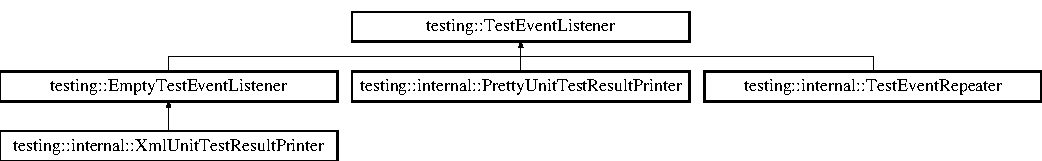
\includegraphics[height=2.162162cm]{classtesting_1_1TestEventListener}
\end{center}
\end{figure}
\subsection*{Membros públicos}
\begin{DoxyCompactItemize}
\item 
\hypertarget{classtesting_1_1TestEventListener_a5f6c84f39851e8a603a2d2e10063816b}{virtual void {\bfseries On\-Test\-Program\-Start} (const \hyperlink{classtesting_1_1UnitTest}{Unit\-Test} \&unit\-\_\-test)=0}\label{classtesting_1_1TestEventListener_a5f6c84f39851e8a603a2d2e10063816b}

\item 
\hypertarget{classtesting_1_1TestEventListener_a60cc09b7907cb329d152eb5e7133bdeb}{virtual void {\bfseries On\-Test\-Iteration\-Start} (const \hyperlink{classtesting_1_1UnitTest}{Unit\-Test} \&unit\-\_\-test, int iteration)=0}\label{classtesting_1_1TestEventListener_a60cc09b7907cb329d152eb5e7133bdeb}

\item 
\hypertarget{classtesting_1_1TestEventListener_aa6502e534919605be45f26a6daf9a40c}{virtual void {\bfseries On\-Environments\-Set\-Up\-Start} (const \hyperlink{classtesting_1_1UnitTest}{Unit\-Test} \&unit\-\_\-test)=0}\label{classtesting_1_1TestEventListener_aa6502e534919605be45f26a6daf9a40c}

\item 
\hypertarget{classtesting_1_1TestEventListener_aaa1021d75f5dbf3f05c829c1cc520341}{virtual void {\bfseries On\-Environments\-Set\-Up\-End} (const \hyperlink{classtesting_1_1UnitTest}{Unit\-Test} \&unit\-\_\-test)=0}\label{classtesting_1_1TestEventListener_aaa1021d75f5dbf3f05c829c1cc520341}

\item 
\hypertarget{classtesting_1_1TestEventListener_ab4ed885d63f5bbff8076c1329b3dfe36}{virtual void {\bfseries On\-Test\-Case\-Start} (const \hyperlink{classtesting_1_1TestCase}{Test\-Case} \&test\-\_\-case)=0}\label{classtesting_1_1TestEventListener_ab4ed885d63f5bbff8076c1329b3dfe36}

\item 
\hypertarget{classtesting_1_1TestEventListener_ab4f6a0ca16ae75daf385b3b5914e1048}{virtual void {\bfseries On\-Test\-Start} (const \hyperlink{classtesting_1_1TestInfo}{Test\-Info} \&test\-\_\-info)=0}\label{classtesting_1_1TestEventListener_ab4f6a0ca16ae75daf385b3b5914e1048}

\item 
\hypertarget{classtesting_1_1TestEventListener_a054f8705c883fa120b91473aff38f2ee}{virtual void {\bfseries On\-Test\-Part\-Result} (const \hyperlink{classtesting_1_1TestPartResult}{Test\-Part\-Result} \&test\-\_\-part\-\_\-result)=0}\label{classtesting_1_1TestEventListener_a054f8705c883fa120b91473aff38f2ee}

\item 
\hypertarget{classtesting_1_1TestEventListener_abb1c44525ef038500608b5dc2f17099b}{virtual void {\bfseries On\-Test\-End} (const \hyperlink{classtesting_1_1TestInfo}{Test\-Info} \&test\-\_\-info)=0}\label{classtesting_1_1TestEventListener_abb1c44525ef038500608b5dc2f17099b}

\item 
\hypertarget{classtesting_1_1TestEventListener_ae61985e2ef76ac78379b077be57a9c36}{virtual void {\bfseries On\-Test\-Case\-End} (const \hyperlink{classtesting_1_1TestCase}{Test\-Case} \&test\-\_\-case)=0}\label{classtesting_1_1TestEventListener_ae61985e2ef76ac78379b077be57a9c36}

\item 
\hypertarget{classtesting_1_1TestEventListener_a468b5e6701bcb86cb2c956caadbba5e4}{virtual void {\bfseries On\-Environments\-Tear\-Down\-Start} (const \hyperlink{classtesting_1_1UnitTest}{Unit\-Test} \&unit\-\_\-test)=0}\label{classtesting_1_1TestEventListener_a468b5e6701bcb86cb2c956caadbba5e4}

\item 
\hypertarget{classtesting_1_1TestEventListener_a9ea04fa7f447865ba76df35e12ba2092}{virtual void {\bfseries On\-Environments\-Tear\-Down\-End} (const \hyperlink{classtesting_1_1UnitTest}{Unit\-Test} \&unit\-\_\-test)=0}\label{classtesting_1_1TestEventListener_a9ea04fa7f447865ba76df35e12ba2092}

\item 
\hypertarget{classtesting_1_1TestEventListener_a550fdb3e55726e4cefa09f5697941425}{virtual void {\bfseries On\-Test\-Iteration\-End} (const \hyperlink{classtesting_1_1UnitTest}{Unit\-Test} \&unit\-\_\-test, int iteration)=0}\label{classtesting_1_1TestEventListener_a550fdb3e55726e4cefa09f5697941425}

\item 
\hypertarget{classtesting_1_1TestEventListener_ad15b6246d94c268e233487a86463ef3d}{virtual void {\bfseries On\-Test\-Program\-End} (const \hyperlink{classtesting_1_1UnitTest}{Unit\-Test} \&unit\-\_\-test)=0}\label{classtesting_1_1TestEventListener_ad15b6246d94c268e233487a86463ef3d}

\end{DoxyCompactItemize}


A documentação para esta classe foi gerada a partir do seguinte ficheiro\-:\begin{DoxyCompactItemize}
\item 
include/gtest/gtest.\-h\end{DoxyCompactItemize}

\hypertarget{classtesting_1_1TestEventListeners}{\section{Referência à classe testing\-:\-:Test\-Event\-Listeners}
\label{classtesting_1_1TestEventListeners}\index{testing\-::\-Test\-Event\-Listeners@{testing\-::\-Test\-Event\-Listeners}}
}
\subsection*{Membros públicos}
\begin{DoxyCompactItemize}
\item 
\hypertarget{classtesting_1_1TestEventListeners_a1207dce74d64c1c39ffa6105560536a0}{void {\bfseries Append} (\hyperlink{classtesting_1_1TestEventListener}{Test\-Event\-Listener} $\ast$listener)}\label{classtesting_1_1TestEventListeners_a1207dce74d64c1c39ffa6105560536a0}

\item 
\hypertarget{classtesting_1_1TestEventListeners_a038c9fa1975f84d6f3d25b52bc7bccdd}{\hyperlink{classtesting_1_1TestEventListener}{Test\-Event\-Listener} $\ast$ {\bfseries Release} (\hyperlink{classtesting_1_1TestEventListener}{Test\-Event\-Listener} $\ast$listener)}\label{classtesting_1_1TestEventListeners_a038c9fa1975f84d6f3d25b52bc7bccdd}

\item 
\hypertarget{classtesting_1_1TestEventListeners_a0a69b6a19e27d53d9ef4683c05e9f75a}{\hyperlink{classtesting_1_1TestEventListener}{Test\-Event\-Listener} $\ast$ {\bfseries default\-\_\-result\-\_\-printer} () const }\label{classtesting_1_1TestEventListeners_a0a69b6a19e27d53d9ef4683c05e9f75a}

\item 
\hypertarget{classtesting_1_1TestEventListeners_a9867c9af50e8d2934a2475286c7cebc5}{\hyperlink{classtesting_1_1TestEventListener}{Test\-Event\-Listener} $\ast$ {\bfseries default\-\_\-xml\-\_\-generator} () const }\label{classtesting_1_1TestEventListeners_a9867c9af50e8d2934a2475286c7cebc5}

\end{DoxyCompactItemize}
\subsection*{Amigos}
\begin{DoxyCompactItemize}
\item 
\hypertarget{classtesting_1_1TestEventListeners_aff779e55b06adfa7c0088bd10253f0f0}{class {\bfseries Test\-Case}}\label{classtesting_1_1TestEventListeners_aff779e55b06adfa7c0088bd10253f0f0}

\item 
\hypertarget{classtesting_1_1TestEventListeners_a4c49c2cdb6c328e6b709b4542f23de3c}{class {\bfseries Test\-Info}}\label{classtesting_1_1TestEventListeners_a4c49c2cdb6c328e6b709b4542f23de3c}

\item 
\hypertarget{classtesting_1_1TestEventListeners_abae39633da9932847b41cb80efd62115}{class {\bfseries internal\-::\-Default\-Global\-Test\-Part\-Result\-Reporter}}\label{classtesting_1_1TestEventListeners_abae39633da9932847b41cb80efd62115}

\item 
\hypertarget{classtesting_1_1TestEventListeners_afddba49fdf3f493532b4d5efb9814f4e}{class {\bfseries internal\-::\-No\-Exec\-Death\-Test}}\label{classtesting_1_1TestEventListeners_afddba49fdf3f493532b4d5efb9814f4e}

\item 
\hypertarget{classtesting_1_1TestEventListeners_addbc107b6b445617c880182bd4f44cf9}{class {\bfseries internal\-::\-Test\-Event\-Listeners\-Accessor}}\label{classtesting_1_1TestEventListeners_addbc107b6b445617c880182bd4f44cf9}

\item 
\hypertarget{classtesting_1_1TestEventListeners_acc0a5e7573fd6ae7ad1878613bb86853}{class {\bfseries internal\-::\-Unit\-Test\-Impl}}\label{classtesting_1_1TestEventListeners_acc0a5e7573fd6ae7ad1878613bb86853}

\end{DoxyCompactItemize}


A documentação para esta classe foi gerada a partir dos seguintes ficheiros\-:\begin{DoxyCompactItemize}
\item 
include/gtest/gtest.\-h\item 
src/gtest.\-cc\end{DoxyCompactItemize}

\hypertarget{classtesting_1_1internal_1_1TestEventRepeater}{\section{Referência à classe testing\-:\-:internal\-:\-:Test\-Event\-Repeater}
\label{classtesting_1_1internal_1_1TestEventRepeater}\index{testing\-::internal\-::\-Test\-Event\-Repeater@{testing\-::internal\-::\-Test\-Event\-Repeater}}
}
Diagrama de heranças da classe testing\-:\-:internal\-:\-:Test\-Event\-Repeater\begin{figure}[H]
\begin{center}
\leavevmode
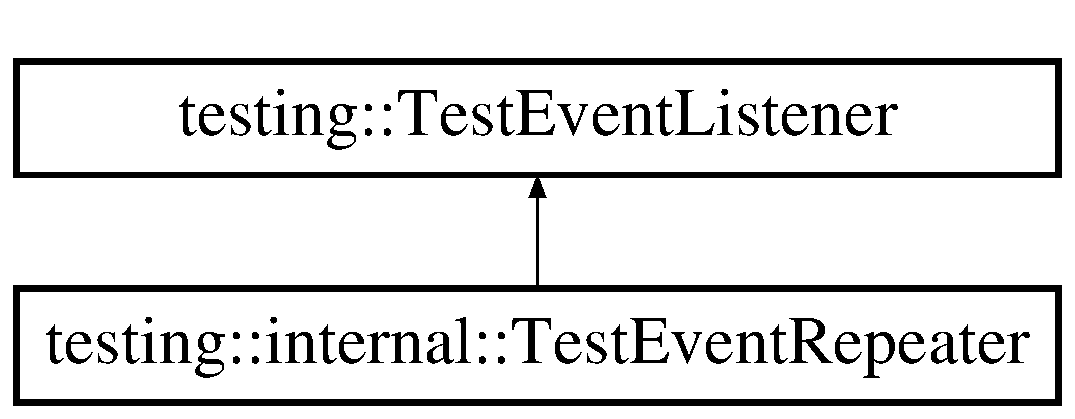
\includegraphics[height=2.000000cm]{classtesting_1_1internal_1_1TestEventRepeater}
\end{center}
\end{figure}
\subsection*{Membros públicos}
\begin{DoxyCompactItemize}
\item 
\hypertarget{classtesting_1_1internal_1_1TestEventRepeater_ad154ce021881721a5c46994316b14cb1}{void {\bfseries Append} (Test\-Event\-Listener $\ast$listener)}\label{classtesting_1_1internal_1_1TestEventRepeater_ad154ce021881721a5c46994316b14cb1}

\item 
\hypertarget{classtesting_1_1internal_1_1TestEventRepeater_ac77a3d127e4726e11694e4ee9cf3b793}{Test\-Event\-Listener $\ast$ {\bfseries Release} (Test\-Event\-Listener $\ast$listener)}\label{classtesting_1_1internal_1_1TestEventRepeater_ac77a3d127e4726e11694e4ee9cf3b793}

\item 
\hypertarget{classtesting_1_1internal_1_1TestEventRepeater_a65c4a855a505ff74c843cf50ad56b4c1}{bool {\bfseries forwarding\-\_\-enabled} () const }\label{classtesting_1_1internal_1_1TestEventRepeater_a65c4a855a505ff74c843cf50ad56b4c1}

\item 
\hypertarget{classtesting_1_1internal_1_1TestEventRepeater_a86c52e311b70598a385a0589277e92e0}{void {\bfseries set\-\_\-forwarding\-\_\-enabled} (bool enable)}\label{classtesting_1_1internal_1_1TestEventRepeater_a86c52e311b70598a385a0589277e92e0}

\item 
\hypertarget{classtesting_1_1internal_1_1TestEventRepeater_a15ee2ff051063088d3a89a266d5ffcc4}{virtual void {\bfseries On\-Test\-Program\-Start} (const Unit\-Test \&unit\-\_\-test)}\label{classtesting_1_1internal_1_1TestEventRepeater_a15ee2ff051063088d3a89a266d5ffcc4}

\item 
\hypertarget{classtesting_1_1internal_1_1TestEventRepeater_a4062b3f070bb6531ab8494c13d3635d3}{virtual void {\bfseries On\-Test\-Iteration\-Start} (const Unit\-Test \&unit\-\_\-test, int iteration)}\label{classtesting_1_1internal_1_1TestEventRepeater_a4062b3f070bb6531ab8494c13d3635d3}

\item 
\hypertarget{classtesting_1_1internal_1_1TestEventRepeater_ae71819925adec0471fa7abc5072b8244}{virtual void {\bfseries On\-Environments\-Set\-Up\-Start} (const Unit\-Test \&unit\-\_\-test)}\label{classtesting_1_1internal_1_1TestEventRepeater_ae71819925adec0471fa7abc5072b8244}

\item 
\hypertarget{classtesting_1_1internal_1_1TestEventRepeater_a3a92696df942dc92f985e52fddd6d303}{virtual void {\bfseries On\-Environments\-Set\-Up\-End} (const Unit\-Test \&unit\-\_\-test)}\label{classtesting_1_1internal_1_1TestEventRepeater_a3a92696df942dc92f985e52fddd6d303}

\item 
\hypertarget{classtesting_1_1internal_1_1TestEventRepeater_a70124c738caa338bcd723eb2a51c8b3e}{virtual void {\bfseries On\-Test\-Case\-Start} (const Test\-Case \&test\-\_\-case)}\label{classtesting_1_1internal_1_1TestEventRepeater_a70124c738caa338bcd723eb2a51c8b3e}

\item 
\hypertarget{classtesting_1_1internal_1_1TestEventRepeater_a70d694ca5010cc86cd458f7f529e6fbe}{virtual void {\bfseries On\-Test\-Start} (const Test\-Info \&test\-\_\-info)}\label{classtesting_1_1internal_1_1TestEventRepeater_a70d694ca5010cc86cd458f7f529e6fbe}

\item 
\hypertarget{classtesting_1_1internal_1_1TestEventRepeater_ac8fb21da6802b1ebab9cad3eee9150eb}{virtual void {\bfseries On\-Test\-Part\-Result} (const Test\-Part\-Result \&result)}\label{classtesting_1_1internal_1_1TestEventRepeater_ac8fb21da6802b1ebab9cad3eee9150eb}

\item 
\hypertarget{classtesting_1_1internal_1_1TestEventRepeater_aa0f13bded9369aae1c78583d7276f8b1}{virtual void {\bfseries On\-Test\-End} (const Test\-Info \&test\-\_\-info)}\label{classtesting_1_1internal_1_1TestEventRepeater_aa0f13bded9369aae1c78583d7276f8b1}

\item 
\hypertarget{classtesting_1_1internal_1_1TestEventRepeater_a0a335e1c3957a8c699ed56e37ea7b978}{virtual void {\bfseries On\-Test\-Case\-End} (const Test\-Case \&test\-\_\-case)}\label{classtesting_1_1internal_1_1TestEventRepeater_a0a335e1c3957a8c699ed56e37ea7b978}

\item 
\hypertarget{classtesting_1_1internal_1_1TestEventRepeater_a30db75df2d9a65d787f31e16004613c2}{virtual void {\bfseries On\-Environments\-Tear\-Down\-Start} (const Unit\-Test \&unit\-\_\-test)}\label{classtesting_1_1internal_1_1TestEventRepeater_a30db75df2d9a65d787f31e16004613c2}

\item 
\hypertarget{classtesting_1_1internal_1_1TestEventRepeater_a8428220c4cf9f0cea2dfd9a70f07ab7f}{virtual void {\bfseries On\-Environments\-Tear\-Down\-End} (const Unit\-Test \&unit\-\_\-test)}\label{classtesting_1_1internal_1_1TestEventRepeater_a8428220c4cf9f0cea2dfd9a70f07ab7f}

\item 
\hypertarget{classtesting_1_1internal_1_1TestEventRepeater_a94253e3c11753328e8a031f39352708f}{virtual void {\bfseries On\-Test\-Iteration\-End} (const Unit\-Test \&unit\-\_\-test, int iteration)}\label{classtesting_1_1internal_1_1TestEventRepeater_a94253e3c11753328e8a031f39352708f}

\item 
\hypertarget{classtesting_1_1internal_1_1TestEventRepeater_a4622616259747dbcc23f5ee39ef99ec0}{virtual void {\bfseries On\-Test\-Program\-End} (const Unit\-Test \&unit\-\_\-test)}\label{classtesting_1_1internal_1_1TestEventRepeater_a4622616259747dbcc23f5ee39ef99ec0}

\end{DoxyCompactItemize}


A documentação para esta classe foi gerada a partir do seguinte ficheiro\-:\begin{DoxyCompactItemize}
\item 
src/gtest.\-cc\end{DoxyCompactItemize}

\hypertarget{classtesting_1_1internal_1_1TestFactoryBase}{\section{Referência à classe testing\-:\-:internal\-:\-:Test\-Factory\-Base}
\label{classtesting_1_1internal_1_1TestFactoryBase}\index{testing\-::internal\-::\-Test\-Factory\-Base@{testing\-::internal\-::\-Test\-Factory\-Base}}
}
Diagrama de heranças da classe testing\-:\-:internal\-:\-:Test\-Factory\-Base\begin{figure}[H]
\begin{center}
\leavevmode
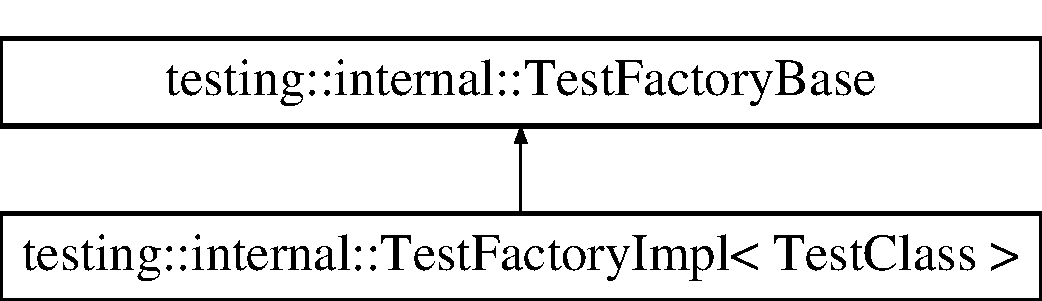
\includegraphics[height=2.000000cm]{classtesting_1_1internal_1_1TestFactoryBase}
\end{center}
\end{figure}
\subsection*{Membros públicos}
\begin{DoxyCompactItemize}
\item 
\hypertarget{classtesting_1_1internal_1_1TestFactoryBase_a07ac3ca0b196cdb092da0bb186b7c030}{virtual \hyperlink{classtesting_1_1Test}{Test} $\ast$ {\bfseries Create\-Test} ()=0}\label{classtesting_1_1internal_1_1TestFactoryBase_a07ac3ca0b196cdb092da0bb186b7c030}

\end{DoxyCompactItemize}


A documentação para esta classe foi gerada a partir do seguinte ficheiro\-:\begin{DoxyCompactItemize}
\item 
include/gtest/internal/gtest-\/internal.\-h\end{DoxyCompactItemize}

\hypertarget{classtesting_1_1internal_1_1TestFactoryImpl}{\section{Referência à classe Template testing\-:\-:internal\-:\-:Test\-Factory\-Impl$<$ Test\-Class $>$}
\label{classtesting_1_1internal_1_1TestFactoryImpl}\index{testing\-::internal\-::\-Test\-Factory\-Impl$<$ Test\-Class $>$@{testing\-::internal\-::\-Test\-Factory\-Impl$<$ Test\-Class $>$}}
}
Diagrama de heranças da classe testing\-:\-:internal\-:\-:Test\-Factory\-Impl$<$ Test\-Class $>$\begin{figure}[H]
\begin{center}
\leavevmode
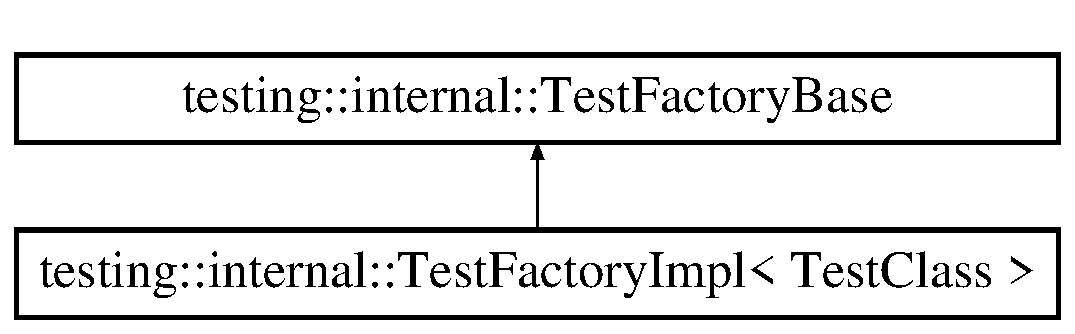
\includegraphics[height=2.000000cm]{classtesting_1_1internal_1_1TestFactoryImpl}
\end{center}
\end{figure}
\subsection*{Membros públicos}
\begin{DoxyCompactItemize}
\item 
\hypertarget{classtesting_1_1internal_1_1TestFactoryImpl_a8860c89bdb06450a5d5e8137ebd9d775}{virtual \hyperlink{classtesting_1_1Test}{Test} $\ast$ {\bfseries Create\-Test} ()}\label{classtesting_1_1internal_1_1TestFactoryImpl_a8860c89bdb06450a5d5e8137ebd9d775}

\end{DoxyCompactItemize}


A documentação para esta classe foi gerada a partir do seguinte ficheiro\-:\begin{DoxyCompactItemize}
\item 
include/gtest/internal/gtest-\/internal.\-h\end{DoxyCompactItemize}

\hypertarget{classtesting_1_1TestInfo}{\section{Referência à classe testing\-:\-:Test\-Info}
\label{classtesting_1_1TestInfo}\index{testing\-::\-Test\-Info@{testing\-::\-Test\-Info}}
}
\subsection*{Membros públicos}
\begin{DoxyCompactItemize}
\item 
\hypertarget{classtesting_1_1TestInfo_a26d22556d04b94c9cd15e28d74fef91c}{const char $\ast$ {\bfseries test\-\_\-case\-\_\-name} () const }\label{classtesting_1_1TestInfo_a26d22556d04b94c9cd15e28d74fef91c}

\item 
\hypertarget{classtesting_1_1TestInfo_ab3d24cad310f0cde29a80b9a83949ff5}{const char $\ast$ {\bfseries name} () const }\label{classtesting_1_1TestInfo_ab3d24cad310f0cde29a80b9a83949ff5}

\item 
\hypertarget{classtesting_1_1TestInfo_af15d5c533a7237ffc183bc4c924dfcf4}{const char $\ast$ {\bfseries type\-\_\-param} () const }\label{classtesting_1_1TestInfo_af15d5c533a7237ffc183bc4c924dfcf4}

\item 
\hypertarget{classtesting_1_1TestInfo_a9671fbc0effcb32e98803888dc166a66}{const char $\ast$ {\bfseries value\-\_\-param} () const }\label{classtesting_1_1TestInfo_a9671fbc0effcb32e98803888dc166a66}

\item 
\hypertarget{classtesting_1_1TestInfo_a240c9fb051d7b0586ed380c6b4e729e4}{bool {\bfseries should\-\_\-run} () const }\label{classtesting_1_1TestInfo_a240c9fb051d7b0586ed380c6b4e729e4}

\item 
\hypertarget{classtesting_1_1TestInfo_a7ad90aeebb1d6fe3a43c6e3e3427e382}{bool {\bfseries is\-\_\-reportable} () const }\label{classtesting_1_1TestInfo_a7ad90aeebb1d6fe3a43c6e3e3427e382}

\item 
\hypertarget{classtesting_1_1TestInfo_addea8766df3b8abe4cc4103218a49a65}{const \hyperlink{classtesting_1_1TestResult}{Test\-Result} $\ast$ {\bfseries result} () const }\label{classtesting_1_1TestInfo_addea8766df3b8abe4cc4103218a49a65}

\end{DoxyCompactItemize}
\subsection*{Amigos}
\begin{DoxyCompactItemize}
\item 
\hypertarget{classtesting_1_1TestInfo_a5b78b1c2e1fa07ffed92da365593eaa4}{class {\bfseries Test}}\label{classtesting_1_1TestInfo_a5b78b1c2e1fa07ffed92da365593eaa4}

\item 
\hypertarget{classtesting_1_1TestInfo_aff779e55b06adfa7c0088bd10253f0f0}{class {\bfseries Test\-Case}}\label{classtesting_1_1TestInfo_aff779e55b06adfa7c0088bd10253f0f0}

\item 
\hypertarget{classtesting_1_1TestInfo_acc0a5e7573fd6ae7ad1878613bb86853}{class {\bfseries internal\-::\-Unit\-Test\-Impl}}\label{classtesting_1_1TestInfo_acc0a5e7573fd6ae7ad1878613bb86853}

\item 
\hypertarget{classtesting_1_1TestInfo_adc037d188dab349a94868991955c9cd4}{class {\bfseries internal\-::\-Streaming\-Listener\-Test}}\label{classtesting_1_1TestInfo_adc037d188dab349a94868991955c9cd4}

\item 
\hypertarget{classtesting_1_1TestInfo_a3e27fa5e97044d379b1e3b2a753f56f8}{\hyperlink{classtesting_1_1TestInfo}{Test\-Info} $\ast$ {\bfseries internal\-::\-Make\-And\-Register\-Test\-Info} (const char $\ast$test\-\_\-case\-\_\-name, const char $\ast$name, const char $\ast$type\-\_\-param, const char $\ast$value\-\_\-param, internal\-::\-Type\-Id fixture\-\_\-class\-\_\-id, Test\-::\-Set\-Up\-Test\-Case\-Func set\-\_\-up\-\_\-tc, Test\-::\-Tear\-Down\-Test\-Case\-Func tear\-\_\-down\-\_\-tc, \hyperlink{classtesting_1_1internal_1_1TestFactoryBase}{internal\-::\-Test\-Factory\-Base} $\ast$factory)}\label{classtesting_1_1TestInfo_a3e27fa5e97044d379b1e3b2a753f56f8}

\end{DoxyCompactItemize}


A documentação para esta classe foi gerada a partir dos seguintes ficheiros\-:\begin{DoxyCompactItemize}
\item 
include/gtest/gtest.\-h\item 
src/gtest.\-cc\end{DoxyCompactItemize}

\hypertarget{classtesting_1_1TestPartResult}{\section{Referência à classe testing\-:\-:Test\-Part\-Result}
\label{classtesting_1_1TestPartResult}\index{testing\-::\-Test\-Part\-Result@{testing\-::\-Test\-Part\-Result}}
}
\subsection*{Tipos Públicos}
\begin{DoxyCompactItemize}
\item 
enum {\bfseries Type} \{ {\bfseries k\-Success}, 
{\bfseries k\-Non\-Fatal\-Failure}, 
{\bfseries k\-Fatal\-Failure}
 \}
\end{DoxyCompactItemize}
\subsection*{Membros públicos}
\begin{DoxyCompactItemize}
\item 
\hypertarget{classtesting_1_1TestPartResult_a6409eb519c1cd514aab2426c8f40737f}{{\bfseries Test\-Part\-Result} (Type a\-\_\-type, const char $\ast$a\-\_\-file\-\_\-name, int a\-\_\-line\-\_\-number, const char $\ast$a\-\_\-message)}\label{classtesting_1_1TestPartResult_a6409eb519c1cd514aab2426c8f40737f}

\item 
\hypertarget{classtesting_1_1TestPartResult_ae852bf8693f066078c74c34345531940}{Type {\bfseries type} () const }\label{classtesting_1_1TestPartResult_ae852bf8693f066078c74c34345531940}

\item 
\hypertarget{classtesting_1_1TestPartResult_a5d8742dc28ddb880cd2391edb9fc2c9b}{const char $\ast$ {\bfseries file\-\_\-name} () const }\label{classtesting_1_1TestPartResult_a5d8742dc28ddb880cd2391edb9fc2c9b}

\item 
\hypertarget{classtesting_1_1TestPartResult_a174900cf4403d23784af34f50e7b0a46}{int {\bfseries line\-\_\-number} () const }\label{classtesting_1_1TestPartResult_a174900cf4403d23784af34f50e7b0a46}

\item 
\hypertarget{classtesting_1_1TestPartResult_af0d4f960b453ce087c581fe13817b2a3}{const char $\ast$ {\bfseries summary} () const }\label{classtesting_1_1TestPartResult_af0d4f960b453ce087c581fe13817b2a3}

\item 
\hypertarget{classtesting_1_1TestPartResult_aae73962246be4d200e2c1d04246a708a}{const char $\ast$ {\bfseries message} () const }\label{classtesting_1_1TestPartResult_aae73962246be4d200e2c1d04246a708a}

\item 
\hypertarget{classtesting_1_1TestPartResult_a901bd62d9fbe7f39826a9d02ab2bdaec}{bool {\bfseries passed} () const }\label{classtesting_1_1TestPartResult_a901bd62d9fbe7f39826a9d02ab2bdaec}

\item 
\hypertarget{classtesting_1_1TestPartResult_aaf835515fb53eb1aa01c1798b05e61f6}{bool {\bfseries failed} () const }\label{classtesting_1_1TestPartResult_aaf835515fb53eb1aa01c1798b05e61f6}

\item 
\hypertarget{classtesting_1_1TestPartResult_a7bb08c87fbc1664f9fcca1504339ed29}{bool {\bfseries nonfatally\-\_\-failed} () const }\label{classtesting_1_1TestPartResult_a7bb08c87fbc1664f9fcca1504339ed29}

\item 
\hypertarget{classtesting_1_1TestPartResult_a34d31718b5fc6c06f73d03e8dbb1aa9e}{bool {\bfseries fatally\-\_\-failed} () const }\label{classtesting_1_1TestPartResult_a34d31718b5fc6c06f73d03e8dbb1aa9e}

\end{DoxyCompactItemize}


A documentação para esta classe foi gerada a partir dos seguintes ficheiros\-:\begin{DoxyCompactItemize}
\item 
include/gtest/gtest-\/test-\/part.\-h\item 
src/gtest-\/test-\/part.\-cc\end{DoxyCompactItemize}

\hypertarget{classtesting_1_1TestPartResultArray}{\section{Referência à classe testing\-:\-:Test\-Part\-Result\-Array}
\label{classtesting_1_1TestPartResultArray}\index{testing\-::\-Test\-Part\-Result\-Array@{testing\-::\-Test\-Part\-Result\-Array}}
}
\subsection*{Membros públicos}
\begin{DoxyCompactItemize}
\item 
\hypertarget{classtesting_1_1TestPartResultArray_a01844bd505b18a666324617a1b459558}{void {\bfseries Append} (const \hyperlink{classtesting_1_1TestPartResult}{Test\-Part\-Result} \&result)}\label{classtesting_1_1TestPartResultArray_a01844bd505b18a666324617a1b459558}

\item 
\hypertarget{classtesting_1_1TestPartResultArray_a799a09c9ad8c1c8875400af78efe4b17}{const \hyperlink{classtesting_1_1TestPartResult}{Test\-Part\-Result} \& {\bfseries Get\-Test\-Part\-Result} (int index) const }\label{classtesting_1_1TestPartResultArray_a799a09c9ad8c1c8875400af78efe4b17}

\item 
\hypertarget{classtesting_1_1TestPartResultArray_acd805ad4edda06d983456b2a30760dce}{int {\bfseries size} () const }\label{classtesting_1_1TestPartResultArray_acd805ad4edda06d983456b2a30760dce}

\end{DoxyCompactItemize}


A documentação para esta classe foi gerada a partir dos seguintes ficheiros\-:\begin{DoxyCompactItemize}
\item 
include/gtest/gtest-\/test-\/part.\-h\item 
src/gtest-\/test-\/part.\-cc\end{DoxyCompactItemize}

\hypertarget{classtesting_1_1TestPartResultReporterInterface}{\section{Referência à classe testing\-:\-:Test\-Part\-Result\-Reporter\-Interface}
\label{classtesting_1_1TestPartResultReporterInterface}\index{testing\-::\-Test\-Part\-Result\-Reporter\-Interface@{testing\-::\-Test\-Part\-Result\-Reporter\-Interface}}
}
Diagrama de heranças da classe testing\-:\-:Test\-Part\-Result\-Reporter\-Interface\begin{figure}[H]
\begin{center}
\leavevmode
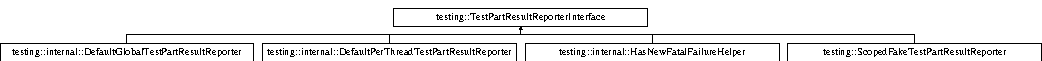
\includegraphics[height=0.825959cm]{classtesting_1_1TestPartResultReporterInterface}
\end{center}
\end{figure}
\subsection*{Membros públicos}
\begin{DoxyCompactItemize}
\item 
\hypertarget{classtesting_1_1TestPartResultReporterInterface_aa2f920e7a5a0a6d0faf19e3727928c22}{virtual void {\bfseries Report\-Test\-Part\-Result} (const \hyperlink{classtesting_1_1TestPartResult}{Test\-Part\-Result} \&result)=0}\label{classtesting_1_1TestPartResultReporterInterface_aa2f920e7a5a0a6d0faf19e3727928c22}

\end{DoxyCompactItemize}


A documentação para esta classe foi gerada a partir do seguinte ficheiro\-:\begin{DoxyCompactItemize}
\item 
include/gtest/gtest-\/test-\/part.\-h\end{DoxyCompactItemize}

\hypertarget{classtesting_1_1TestProperty}{\section{Referência à classe testing\-:\-:Test\-Property}
\label{classtesting_1_1TestProperty}\index{testing\-::\-Test\-Property@{testing\-::\-Test\-Property}}
}
\subsection*{Membros públicos}
\begin{DoxyCompactItemize}
\item 
\hypertarget{classtesting_1_1TestProperty_a25a0ccf1c75a92af46a48d3c2a873e6d}{{\bfseries Test\-Property} (const std\-::string \&a\-\_\-key, const std\-::string \&a\-\_\-value)}\label{classtesting_1_1TestProperty_a25a0ccf1c75a92af46a48d3c2a873e6d}

\item 
\hypertarget{classtesting_1_1TestProperty_a2c569d47685b89aa64e737fb11df3aba}{const char $\ast$ {\bfseries key} () const }\label{classtesting_1_1TestProperty_a2c569d47685b89aa64e737fb11df3aba}

\item 
\hypertarget{classtesting_1_1TestProperty_ad46323c18491f365d72d8a4288f54bd6}{const char $\ast$ {\bfseries value} () const }\label{classtesting_1_1TestProperty_ad46323c18491f365d72d8a4288f54bd6}

\item 
\hypertarget{classtesting_1_1TestProperty_a377245335d9f614cd06d1650e3358e1d}{void {\bfseries Set\-Value} (const std\-::string \&new\-\_\-value)}\label{classtesting_1_1TestProperty_a377245335d9f614cd06d1650e3358e1d}

\end{DoxyCompactItemize}


A documentação para esta classe foi gerada a partir do seguinte ficheiro\-:\begin{DoxyCompactItemize}
\item 
include/gtest/gtest.\-h\end{DoxyCompactItemize}

\hypertarget{classtesting_1_1internal_1_1TestPropertyKeyIs}{\section{Referência à classe testing\-:\-:internal\-:\-:Test\-Property\-Key\-Is}
\label{classtesting_1_1internal_1_1TestPropertyKeyIs}\index{testing\-::internal\-::\-Test\-Property\-Key\-Is@{testing\-::internal\-::\-Test\-Property\-Key\-Is}}
}
\subsection*{Membros públicos}
\begin{DoxyCompactItemize}
\item 
\hypertarget{classtesting_1_1internal_1_1TestPropertyKeyIs_a509ed1271caa1032e40c5d811b3da385}{{\bfseries Test\-Property\-Key\-Is} (const std\-::string \&key)}\label{classtesting_1_1internal_1_1TestPropertyKeyIs_a509ed1271caa1032e40c5d811b3da385}

\item 
\hypertarget{classtesting_1_1internal_1_1TestPropertyKeyIs_aed5dfb89159b3a071a8f3521fa1f8eb0}{bool {\bfseries operator()} (const \hyperlink{classtesting_1_1TestProperty}{Test\-Property} \&test\-\_\-property) const }\label{classtesting_1_1internal_1_1TestPropertyKeyIs_aed5dfb89159b3a071a8f3521fa1f8eb0}

\end{DoxyCompactItemize}


A documentação para esta classe foi gerada a partir do seguinte ficheiro\-:\begin{DoxyCompactItemize}
\item 
src/gtest-\/internal-\/inl.\-h\end{DoxyCompactItemize}

\hypertarget{classtesting_1_1TestResult}{\section{Referência à classe testing\-:\-:Test\-Result}
\label{classtesting_1_1TestResult}\index{testing\-::\-Test\-Result@{testing\-::\-Test\-Result}}
}
\subsection*{Membros públicos}
\begin{DoxyCompactItemize}
\item 
\hypertarget{classtesting_1_1TestResult_ae6a378ec743edfbed55890c955d0adc8}{int {\bfseries total\-\_\-part\-\_\-count} () const }\label{classtesting_1_1TestResult_ae6a378ec743edfbed55890c955d0adc8}

\item 
\hypertarget{classtesting_1_1TestResult_a5075f9d595d51c7cc2f5c0921e622831}{int {\bfseries test\-\_\-property\-\_\-count} () const }\label{classtesting_1_1TestResult_a5075f9d595d51c7cc2f5c0921e622831}

\item 
\hypertarget{classtesting_1_1TestResult_aa46a04342f02ec297357f47288da3ef3}{bool {\bfseries Passed} () const }\label{classtesting_1_1TestResult_aa46a04342f02ec297357f47288da3ef3}

\item 
\hypertarget{classtesting_1_1TestResult_abb5d051bf958071c14020132a4d6cc07}{bool {\bfseries Failed} () const }\label{classtesting_1_1TestResult_abb5d051bf958071c14020132a4d6cc07}

\item 
\hypertarget{classtesting_1_1TestResult_ace61ce992083a9124f9ff0e99a2041cc}{bool {\bfseries Has\-Fatal\-Failure} () const }\label{classtesting_1_1TestResult_ace61ce992083a9124f9ff0e99a2041cc}

\item 
\hypertarget{classtesting_1_1TestResult_a34e6901b9772f51ce4f17a5517c26607}{bool {\bfseries Has\-Nonfatal\-Failure} () const }\label{classtesting_1_1TestResult_a34e6901b9772f51ce4f17a5517c26607}

\item 
\hypertarget{classtesting_1_1TestResult_a582f6383265d0619df812b75499d0616}{Time\-In\-Millis {\bfseries elapsed\-\_\-time} () const }\label{classtesting_1_1TestResult_a582f6383265d0619df812b75499d0616}

\item 
\hypertarget{classtesting_1_1TestResult_a08b680f63d91391db4161f909da2bbcc}{const \hyperlink{classtesting_1_1TestPartResult}{Test\-Part\-Result} \& {\bfseries Get\-Test\-Part\-Result} (int i) const }\label{classtesting_1_1TestResult_a08b680f63d91391db4161f909da2bbcc}

\item 
\hypertarget{classtesting_1_1TestResult_a2cb23a457a444ba85684dd655895f08e}{const \hyperlink{classtesting_1_1TestProperty}{Test\-Property} \& {\bfseries Get\-Test\-Property} (int i) const }\label{classtesting_1_1TestResult_a2cb23a457a444ba85684dd655895f08e}

\end{DoxyCompactItemize}
\subsection*{Amigos}
\begin{DoxyCompactItemize}
\item 
\hypertarget{classtesting_1_1TestResult_a4c49c2cdb6c328e6b709b4542f23de3c}{class {\bfseries Test\-Info}}\label{classtesting_1_1TestResult_a4c49c2cdb6c328e6b709b4542f23de3c}

\item 
\hypertarget{classtesting_1_1TestResult_aff779e55b06adfa7c0088bd10253f0f0}{class {\bfseries Test\-Case}}\label{classtesting_1_1TestResult_aff779e55b06adfa7c0088bd10253f0f0}

\item 
\hypertarget{classtesting_1_1TestResult_a832b4d233efee1a32feb0f4190b30d39}{class {\bfseries Unit\-Test}}\label{classtesting_1_1TestResult_a832b4d233efee1a32feb0f4190b30d39}

\item 
\hypertarget{classtesting_1_1TestResult_abae39633da9932847b41cb80efd62115}{class {\bfseries internal\-::\-Default\-Global\-Test\-Part\-Result\-Reporter}}\label{classtesting_1_1TestResult_abae39633da9932847b41cb80efd62115}

\item 
\hypertarget{classtesting_1_1TestResult_adf5553cae6aea6f8648d47e299237e34}{class {\bfseries internal\-::\-Exec\-Death\-Test}}\label{classtesting_1_1TestResult_adf5553cae6aea6f8648d47e299237e34}

\item 
\hypertarget{classtesting_1_1TestResult_ae762da04e74a0d3b0daded3c5bd4a8e8}{class {\bfseries internal\-::\-Test\-Result\-Accessor}}\label{classtesting_1_1TestResult_ae762da04e74a0d3b0daded3c5bd4a8e8}

\item 
\hypertarget{classtesting_1_1TestResult_acc0a5e7573fd6ae7ad1878613bb86853}{class {\bfseries internal\-::\-Unit\-Test\-Impl}}\label{classtesting_1_1TestResult_acc0a5e7573fd6ae7ad1878613bb86853}

\item 
\hypertarget{classtesting_1_1TestResult_a6aeedc04a0590fcc1b3c5f687dbb0f9f}{class {\bfseries internal\-::\-Windows\-Death\-Test}}\label{classtesting_1_1TestResult_a6aeedc04a0590fcc1b3c5f687dbb0f9f}

\end{DoxyCompactItemize}


A documentação para esta classe foi gerada a partir dos seguintes ficheiros\-:\begin{DoxyCompactItemize}
\item 
include/gtest/gtest.\-h\item 
src/gtest.\-cc\end{DoxyCompactItemize}

\hypertarget{classtesting_1_1internal_1_1TestResultAccessor}{\section{Referência à classe testing\-:\-:internal\-:\-:Test\-Result\-Accessor}
\label{classtesting_1_1internal_1_1TestResultAccessor}\index{testing\-::internal\-::\-Test\-Result\-Accessor@{testing\-::internal\-::\-Test\-Result\-Accessor}}
}
\subsection*{Membros públicos estáticos}
\begin{DoxyCompactItemize}
\item 
\hypertarget{classtesting_1_1internal_1_1TestResultAccessor_abcc4b32d1b201eeef92f0ec0ae161cf9}{static void {\bfseries Record\-Property} (Test\-Result $\ast$test\-\_\-result, const std\-::string \&xml\-\_\-element, const Test\-Property \&property)}\label{classtesting_1_1internal_1_1TestResultAccessor_abcc4b32d1b201eeef92f0ec0ae161cf9}

\item 
\hypertarget{classtesting_1_1internal_1_1TestResultAccessor_a53c626632bac65d82d88e432072b866b}{static void {\bfseries Clear\-Test\-Part\-Results} (Test\-Result $\ast$test\-\_\-result)}\label{classtesting_1_1internal_1_1TestResultAccessor_a53c626632bac65d82d88e432072b866b}

\item 
\hypertarget{classtesting_1_1internal_1_1TestResultAccessor_a55d771904317c1b0cc380104d175f1db}{static const std\-::vector\\*
$<$ testing\-::\-Test\-Part\-Result $>$ \& {\bfseries test\-\_\-part\-\_\-results} (const Test\-Result \&test\-\_\-result)}\label{classtesting_1_1internal_1_1TestResultAccessor_a55d771904317c1b0cc380104d175f1db}

\end{DoxyCompactItemize}


A documentação para esta classe foi gerada a partir do seguinte ficheiro\-:\begin{DoxyCompactItemize}
\item 
src/gtest-\/internal-\/inl.\-h\end{DoxyCompactItemize}

\hypertarget{classtesting_1_1internal_1_1ThreadLocal}{\section{Referência à classe Template testing\-:\-:internal\-:\-:Thread\-Local$<$ T $>$}
\label{classtesting_1_1internal_1_1ThreadLocal}\index{testing\-::internal\-::\-Thread\-Local$<$ T $>$@{testing\-::internal\-::\-Thread\-Local$<$ T $>$}}
}
\subsection*{Membros públicos}
\begin{DoxyCompactItemize}
\item 
\hypertarget{classtesting_1_1internal_1_1ThreadLocal_a85610bdfdbc93a4c56215e0aad7da870}{{\bfseries Thread\-Local} (const T \&value)}\label{classtesting_1_1internal_1_1ThreadLocal_a85610bdfdbc93a4c56215e0aad7da870}

\item 
\hypertarget{classtesting_1_1internal_1_1ThreadLocal_a882f57fed4b074de83693c0c0fe62858}{T $\ast$ {\bfseries pointer} ()}\label{classtesting_1_1internal_1_1ThreadLocal_a882f57fed4b074de83693c0c0fe62858}

\item 
\hypertarget{classtesting_1_1internal_1_1ThreadLocal_af4b33c12fd2da7d43d8654feccca77f7}{const T $\ast$ {\bfseries pointer} () const }\label{classtesting_1_1internal_1_1ThreadLocal_af4b33c12fd2da7d43d8654feccca77f7}

\item 
\hypertarget{classtesting_1_1internal_1_1ThreadLocal_a9cfa47ae6e9e8c19fe8782e2e9c1b13e}{const T \& {\bfseries get} () const }\label{classtesting_1_1internal_1_1ThreadLocal_a9cfa47ae6e9e8c19fe8782e2e9c1b13e}

\item 
\hypertarget{classtesting_1_1internal_1_1ThreadLocal_ab5ebc7ba07426cef7167afa2a7707eb4}{void {\bfseries set} (const T \&value)}\label{classtesting_1_1internal_1_1ThreadLocal_ab5ebc7ba07426cef7167afa2a7707eb4}

\end{DoxyCompactItemize}


A documentação para esta classe foi gerada a partir do seguinte ficheiro\-:\begin{DoxyCompactItemize}
\item 
include/gtest/internal/gtest-\/port.\-h\end{DoxyCompactItemize}

\hypertarget{structtesting_1_1internal_1_1TraceInfo}{\section{Referência à estrutura testing\-:\-:internal\-:\-:Trace\-Info}
\label{structtesting_1_1internal_1_1TraceInfo}\index{testing\-::internal\-::\-Trace\-Info@{testing\-::internal\-::\-Trace\-Info}}
}
\subsection*{Atributos Públicos}
\begin{DoxyCompactItemize}
\item 
\hypertarget{structtesting_1_1internal_1_1TraceInfo_a5d801209d3c0840aa55cfd4b67504254}{const char $\ast$ {\bfseries file}}\label{structtesting_1_1internal_1_1TraceInfo_a5d801209d3c0840aa55cfd4b67504254}

\item 
\hypertarget{structtesting_1_1internal_1_1TraceInfo_ae9d269de1b77f4a3180d0d34acb4d7ff}{int {\bfseries line}}\label{structtesting_1_1internal_1_1TraceInfo_ae9d269de1b77f4a3180d0d34acb4d7ff}

\item 
\hypertarget{structtesting_1_1internal_1_1TraceInfo_a39e74f39ce6d5fdbac799abdb1c27f90}{std\-::string {\bfseries message}}\label{structtesting_1_1internal_1_1TraceInfo_a39e74f39ce6d5fdbac799abdb1c27f90}

\end{DoxyCompactItemize}


A documentação para esta estrutura foi gerada a partir do seguinte ficheiro\-:\begin{DoxyCompactItemize}
\item 
src/gtest-\/internal-\/inl.\-h\end{DoxyCompactItemize}

\hypertarget{classstd_1_1tr1_1_1tuple}{\section{Referência à classe Template std\-:\-:tr1\-:\-:tuple$<$ T0, T1, T2, T3, T4, T5, T6, T7, T8, T9 $>$}
\label{classstd_1_1tr1_1_1tuple}\index{std\-::tr1\-::tuple$<$ T0, T1, T2, T3, T4, T5, T6, T7, T8, T9 $>$@{std\-::tr1\-::tuple$<$ T0, T1, T2, T3, T4, T5, T6, T7, T8, T9 $>$}}
}
\subsection*{Membros públicos}
\begin{DoxyCompactItemize}
\item 
\hypertarget{classstd_1_1tr1_1_1tuple_a5c31ee8e6f548fc37ef814d3db7d273f}{{\bfseries tuple} (G\-T\-E\-S\-T\-\_\-\-B\-Y\-\_\-\-R\-E\-F\-\_\-(T0) f0, G\-T\-E\-S\-T\-\_\-\-B\-Y\-\_\-\-R\-E\-F\-\_\-(T1) f1, G\-T\-E\-S\-T\-\_\-\-B\-Y\-\_\-\-R\-E\-F\-\_\-(T2) f2, G\-T\-E\-S\-T\-\_\-\-B\-Y\-\_\-\-R\-E\-F\-\_\-(T3) f3, G\-T\-E\-S\-T\-\_\-\-B\-Y\-\_\-\-R\-E\-F\-\_\-(T4) f4, G\-T\-E\-S\-T\-\_\-\-B\-Y\-\_\-\-R\-E\-F\-\_\-(T5) f5, G\-T\-E\-S\-T\-\_\-\-B\-Y\-\_\-\-R\-E\-F\-\_\-(T6) f6, G\-T\-E\-S\-T\-\_\-\-B\-Y\-\_\-\-R\-E\-F\-\_\-(T7) f7, G\-T\-E\-S\-T\-\_\-\-B\-Y\-\_\-\-R\-E\-F\-\_\-(T8) f8, G\-T\-E\-S\-T\-\_\-\-B\-Y\-\_\-\-R\-E\-F\-\_\-(T9) f9)}\label{classstd_1_1tr1_1_1tuple_a5c31ee8e6f548fc37ef814d3db7d273f}

\item 
\hypertarget{classstd_1_1tr1_1_1tuple_a70a4e487f56c2f544a40ca81e1b69303}{{\bfseries tuple} (const \hyperlink{classstd_1_1tr1_1_1tuple}{tuple} \&t)}\label{classstd_1_1tr1_1_1tuple_a70a4e487f56c2f544a40ca81e1b69303}

\item 
\hypertarget{classstd_1_1tr1_1_1tuple_a3ecd978bce485352717c801af8a6e113}{{\footnotesize template$<$G\-T\-E\-S\-T\-\_\-10\-\_\-\-T\-Y\-P\-E\-N\-A\-M\-E\-S\-\_\-(\-U) $>$ }\\{\bfseries tuple} (const G\-T\-E\-S\-T\-\_\-10\-\_\-\-T\-U\-P\-L\-E\-\_\-(U)\&t)}\label{classstd_1_1tr1_1_1tuple_a3ecd978bce485352717c801af8a6e113}

\item 
\hypertarget{classstd_1_1tr1_1_1tuple_a2544141b07a65060937e594228ee815a}{\hyperlink{classstd_1_1tr1_1_1tuple}{tuple} \& {\bfseries operator=} (const \hyperlink{classstd_1_1tr1_1_1tuple}{tuple} \&t)}\label{classstd_1_1tr1_1_1tuple_a2544141b07a65060937e594228ee815a}

\item 
\hypertarget{classstd_1_1tr1_1_1tuple_af0df06ea0529f3caa6cbbf9daaa4d341}{{\footnotesize template$<$G\-T\-E\-S\-T\-\_\-10\-\_\-\-T\-Y\-P\-E\-N\-A\-M\-E\-S\-\_\-(\-U) $>$ }\\\hyperlink{classstd_1_1tr1_1_1tuple}{tuple} \& {\bfseries operator=} (const G\-T\-E\-S\-T\-\_\-10\-\_\-\-T\-U\-P\-L\-E\-\_\-(U)\&t)}\label{classstd_1_1tr1_1_1tuple_af0df06ea0529f3caa6cbbf9daaa4d341}

\item 
\hypertarget{classstd_1_1tr1_1_1tuple_aa76d0c02e6f4c6c99f32f9738623f23c}{{\footnotesize template$<$G\-T\-E\-S\-T\-\_\-10\-\_\-\-T\-Y\-P\-E\-N\-A\-M\-E\-S\-\_\-(\-U) $>$ }\\G\-T\-E\-S\-T\-\_\-\-D\-E\-C\-L\-A\-R\-E\-\_\-\-T\-U\-P\-L\-E\-\_\-\-A\-S\-\_\-\-F\-R\-I\-E\-N\-D\-\_\- \\*
\hyperlink{classstd_1_1tr1_1_1tuple}{tuple} \& {\bfseries Copy\-From} (const G\-T\-E\-S\-T\-\_\-10\-\_\-\-T\-U\-P\-L\-E\-\_\-(U)\&t)}\label{classstd_1_1tr1_1_1tuple_aa76d0c02e6f4c6c99f32f9738623f23c}

\end{DoxyCompactItemize}
\subsection*{Atributos Públicos}
\begin{DoxyCompactItemize}
\item 
\hypertarget{classstd_1_1tr1_1_1tuple_a133b02f631ce9c46c8368756d5ce7d68}{T0 {\bfseries f0\-\_\-}}\label{classstd_1_1tr1_1_1tuple_a133b02f631ce9c46c8368756d5ce7d68}

\item 
\hypertarget{classstd_1_1tr1_1_1tuple_a809d974a332969e624830b02d9361107}{T1 {\bfseries f1\-\_\-}}\label{classstd_1_1tr1_1_1tuple_a809d974a332969e624830b02d9361107}

\item 
\hypertarget{classstd_1_1tr1_1_1tuple_a1a3d444570fccf3810322a5cea025993}{T2 {\bfseries f2\-\_\-}}\label{classstd_1_1tr1_1_1tuple_a1a3d444570fccf3810322a5cea025993}

\item 
\hypertarget{classstd_1_1tr1_1_1tuple_a7d1ea537cc17e4c1aa1e4a7b39822c93}{T3 {\bfseries f3\-\_\-}}\label{classstd_1_1tr1_1_1tuple_a7d1ea537cc17e4c1aa1e4a7b39822c93}

\item 
\hypertarget{classstd_1_1tr1_1_1tuple_a893ccbbb34a262058b4cfa5020bbf84e}{T4 {\bfseries f4\-\_\-}}\label{classstd_1_1tr1_1_1tuple_a893ccbbb34a262058b4cfa5020bbf84e}

\item 
\hypertarget{classstd_1_1tr1_1_1tuple_a1fbe806ede11f6e48aff17ce5c7b96a8}{T5 {\bfseries f5\-\_\-}}\label{classstd_1_1tr1_1_1tuple_a1fbe806ede11f6e48aff17ce5c7b96a8}

\item 
\hypertarget{classstd_1_1tr1_1_1tuple_a1b7ddbc9893546b3028ee8f4543534cc}{T6 {\bfseries f6\-\_\-}}\label{classstd_1_1tr1_1_1tuple_a1b7ddbc9893546b3028ee8f4543534cc}

\item 
\hypertarget{classstd_1_1tr1_1_1tuple_a254d543fc3669d5cbd41d5da833b9492}{T7 {\bfseries f7\-\_\-}}\label{classstd_1_1tr1_1_1tuple_a254d543fc3669d5cbd41d5da833b9492}

\item 
\hypertarget{classstd_1_1tr1_1_1tuple_a335bd9d920b8aff1e2a47980bbf274db}{T8 {\bfseries f8\-\_\-}}\label{classstd_1_1tr1_1_1tuple_a335bd9d920b8aff1e2a47980bbf274db}

\item 
\hypertarget{classstd_1_1tr1_1_1tuple_a1b8a389f9e3974be4130f6ba2fbe5234}{T9 {\bfseries f9\-\_\-}}\label{classstd_1_1tr1_1_1tuple_a1b8a389f9e3974be4130f6ba2fbe5234}

\end{DoxyCompactItemize}
\subsection*{Amigos}
\begin{DoxyCompactItemize}
\item 
\hypertarget{classstd_1_1tr1_1_1tuple_aeeed38755abdaa78587dd1eac9ccc950}{{\footnotesize template$<$int k$>$ }\\class {\bfseries gtest\-\_\-internal\-::\-Get}}\label{classstd_1_1tr1_1_1tuple_aeeed38755abdaa78587dd1eac9ccc950}

\end{DoxyCompactItemize}


A documentação para esta classe foi gerada a partir do seguinte ficheiro\-:\begin{DoxyCompactItemize}
\item 
include/gtest/internal/gtest-\/tuple.\-h\end{DoxyCompactItemize}

\hypertarget{classstd_1_1tr1_1_1tuple_3_4}{\section{Referência à classe Template std\-:\-:tr1\-:\-:tuple$<$$>$}
\label{classstd_1_1tr1_1_1tuple_3_4}\index{std\-::tr1\-::tuple$<$$>$@{std\-::tr1\-::tuple$<$$>$}}
}
\subsection*{Membros públicos}
\begin{DoxyCompactItemize}
\item 
\hypertarget{classstd_1_1tr1_1_1tuple_3_4_aa857599acb126134e29dc5e53fd9d1a7}{{\bfseries tuple} (const \hyperlink{classstd_1_1tr1_1_1tuple}{tuple} \&)}\label{classstd_1_1tr1_1_1tuple_3_4_aa857599acb126134e29dc5e53fd9d1a7}

\item 
\hypertarget{classstd_1_1tr1_1_1tuple_3_4_a93ddab6f662662fc49635608619150c8}{\hyperlink{classstd_1_1tr1_1_1tuple}{tuple} \& {\bfseries operator=} (const \hyperlink{classstd_1_1tr1_1_1tuple}{tuple} \&)}\label{classstd_1_1tr1_1_1tuple_3_4_a93ddab6f662662fc49635608619150c8}

\end{DoxyCompactItemize}


A documentação para esta classe foi gerada a partir do seguinte ficheiro\-:\begin{DoxyCompactItemize}
\item 
include/gtest/internal/gtest-\/tuple.\-h\end{DoxyCompactItemize}

\hypertarget{structstd_1_1tr1_1_1tuple__element}{\section{Referência à estrutura Template std\-:\-:tr1\-:\-:tuple\-\_\-element$<$ k, Tuple $>$}
\label{structstd_1_1tr1_1_1tuple__element}\index{std\-::tr1\-::tuple\-\_\-element$<$ k, Tuple $>$@{std\-::tr1\-::tuple\-\_\-element$<$ k, Tuple $>$}}
}


A documentação para esta estrutura foi gerada a partir do seguinte ficheiro\-:\begin{DoxyCompactItemize}
\item 
include/gtest/internal/gtest-\/tuple.\-h\end{DoxyCompactItemize}

\hypertarget{structstd_1_1tr1_1_1tuple__size}{\section{Referência à estrutura Template std\-:\-:tr1\-:\-:tuple\-\_\-size$<$ Tuple $>$}
\label{structstd_1_1tr1_1_1tuple__size}\index{std\-::tr1\-::tuple\-\_\-size$<$ Tuple $>$@{std\-::tr1\-::tuple\-\_\-size$<$ Tuple $>$}}
}


A documentação para esta estrutura foi gerada a partir do seguinte ficheiro\-:\begin{DoxyCompactItemize}
\item 
include/gtest/internal/gtest-\/tuple.\-h\end{DoxyCompactItemize}

\hypertarget{structstd_1_1tr1_1_1tuple__size_3_01GTEST__0__TUPLE___07T_08_01_4}{\section{Referência à estrutura Template std\-:\-:tr1\-:\-:tuple\-\_\-size$<$ G\-T\-E\-S\-T\-\_\-0\-\_\-\-T\-U\-P\-L\-E\-\_\-(T) $>$}
\label{structstd_1_1tr1_1_1tuple__size_3_01GTEST__0__TUPLE___07T_08_01_4}\index{std\-::tr1\-::tuple\-\_\-size$<$ G\-T\-E\-S\-T\-\_\-0\-\_\-\-T\-U\-P\-L\-E\-\_\-(\-T) $>$@{std\-::tr1\-::tuple\-\_\-size$<$ G\-T\-E\-S\-T\-\_\-0\-\_\-\-T\-U\-P\-L\-E\-\_\-(\-T) $>$}}
}
\subsection*{Atributos Públicos Estáticos}
\begin{DoxyCompactItemize}
\item 
\hypertarget{structstd_1_1tr1_1_1tuple__size_3_01GTEST__0__TUPLE___07T_08_01_4_af34d6d0b87d7379b14817a386c1e18ee}{static const int {\bfseries value} = 0}\label{structstd_1_1tr1_1_1tuple__size_3_01GTEST__0__TUPLE___07T_08_01_4_af34d6d0b87d7379b14817a386c1e18ee}

\end{DoxyCompactItemize}


A documentação para esta estrutura foi gerada a partir do seguinte ficheiro\-:\begin{DoxyCompactItemize}
\item 
include/gtest/internal/gtest-\/tuple.\-h\end{DoxyCompactItemize}

\hypertarget{structstd_1_1tr1_1_1tuple__size_3_01GTEST__10__TUPLE___07T_08_01_4}{\section{Referência à estrutura Template std\-:\-:tr1\-:\-:tuple\-\_\-size$<$ G\-T\-E\-S\-T\-\_\-10\-\_\-\-T\-U\-P\-L\-E\-\_\-(T) $>$}
\label{structstd_1_1tr1_1_1tuple__size_3_01GTEST__10__TUPLE___07T_08_01_4}\index{std\-::tr1\-::tuple\-\_\-size$<$ G\-T\-E\-S\-T\-\_\-10\-\_\-\-T\-U\-P\-L\-E\-\_\-(\-T) $>$@{std\-::tr1\-::tuple\-\_\-size$<$ G\-T\-E\-S\-T\-\_\-10\-\_\-\-T\-U\-P\-L\-E\-\_\-(\-T) $>$}}
}
\subsection*{Atributos Públicos Estáticos}
\begin{DoxyCompactItemize}
\item 
\hypertarget{structstd_1_1tr1_1_1tuple__size_3_01GTEST__10__TUPLE___07T_08_01_4_a8181de395f9761be991e4cbdef144373}{static const int {\bfseries value} = 10}\label{structstd_1_1tr1_1_1tuple__size_3_01GTEST__10__TUPLE___07T_08_01_4_a8181de395f9761be991e4cbdef144373}

\end{DoxyCompactItemize}


A documentação para esta estrutura foi gerada a partir do seguinte ficheiro\-:\begin{DoxyCompactItemize}
\item 
include/gtest/internal/gtest-\/tuple.\-h\end{DoxyCompactItemize}

\hypertarget{structstd_1_1tr1_1_1tuple__size_3_01GTEST__1__TUPLE___07T_08_01_4}{\section{Referência à estrutura Template std\-:\-:tr1\-:\-:tuple\-\_\-size$<$ G\-T\-E\-S\-T\-\_\-1\-\_\-\-T\-U\-P\-L\-E\-\_\-(T) $>$}
\label{structstd_1_1tr1_1_1tuple__size_3_01GTEST__1__TUPLE___07T_08_01_4}\index{std\-::tr1\-::tuple\-\_\-size$<$ G\-T\-E\-S\-T\-\_\-1\-\_\-\-T\-U\-P\-L\-E\-\_\-(\-T) $>$@{std\-::tr1\-::tuple\-\_\-size$<$ G\-T\-E\-S\-T\-\_\-1\-\_\-\-T\-U\-P\-L\-E\-\_\-(\-T) $>$}}
}
\subsection*{Atributos Públicos Estáticos}
\begin{DoxyCompactItemize}
\item 
\hypertarget{structstd_1_1tr1_1_1tuple__size_3_01GTEST__1__TUPLE___07T_08_01_4_a02cb0da1163ad7eb74782b8f63420d5a}{static const int {\bfseries value} = 1}\label{structstd_1_1tr1_1_1tuple__size_3_01GTEST__1__TUPLE___07T_08_01_4_a02cb0da1163ad7eb74782b8f63420d5a}

\end{DoxyCompactItemize}


A documentação para esta estrutura foi gerada a partir do seguinte ficheiro\-:\begin{DoxyCompactItemize}
\item 
include/gtest/internal/gtest-\/tuple.\-h\end{DoxyCompactItemize}

\hypertarget{structstd_1_1tr1_1_1tuple__size_3_01GTEST__2__TUPLE___07T_08_01_4}{\section{Referência à estrutura Template std\-:\-:tr1\-:\-:tuple\-\_\-size$<$ G\-T\-E\-S\-T\-\_\-2\-\_\-\-T\-U\-P\-L\-E\-\_\-(T) $>$}
\label{structstd_1_1tr1_1_1tuple__size_3_01GTEST__2__TUPLE___07T_08_01_4}\index{std\-::tr1\-::tuple\-\_\-size$<$ G\-T\-E\-S\-T\-\_\-2\-\_\-\-T\-U\-P\-L\-E\-\_\-(\-T) $>$@{std\-::tr1\-::tuple\-\_\-size$<$ G\-T\-E\-S\-T\-\_\-2\-\_\-\-T\-U\-P\-L\-E\-\_\-(\-T) $>$}}
}
\subsection*{Atributos Públicos Estáticos}
\begin{DoxyCompactItemize}
\item 
\hypertarget{structstd_1_1tr1_1_1tuple__size_3_01GTEST__2__TUPLE___07T_08_01_4_a18545d733fa1f811712aa1153d8ba5d9}{static const int {\bfseries value} = 2}\label{structstd_1_1tr1_1_1tuple__size_3_01GTEST__2__TUPLE___07T_08_01_4_a18545d733fa1f811712aa1153d8ba5d9}

\end{DoxyCompactItemize}


A documentação para esta estrutura foi gerada a partir do seguinte ficheiro\-:\begin{DoxyCompactItemize}
\item 
include/gtest/internal/gtest-\/tuple.\-h\end{DoxyCompactItemize}

\hypertarget{structstd_1_1tr1_1_1tuple__size_3_01GTEST__3__TUPLE___07T_08_01_4}{\section{Referência à estrutura Template std\-:\-:tr1\-:\-:tuple\-\_\-size$<$ G\-T\-E\-S\-T\-\_\-3\-\_\-\-T\-U\-P\-L\-E\-\_\-(T) $>$}
\label{structstd_1_1tr1_1_1tuple__size_3_01GTEST__3__TUPLE___07T_08_01_4}\index{std\-::tr1\-::tuple\-\_\-size$<$ G\-T\-E\-S\-T\-\_\-3\-\_\-\-T\-U\-P\-L\-E\-\_\-(\-T) $>$@{std\-::tr1\-::tuple\-\_\-size$<$ G\-T\-E\-S\-T\-\_\-3\-\_\-\-T\-U\-P\-L\-E\-\_\-(\-T) $>$}}
}
\subsection*{Atributos Públicos Estáticos}
\begin{DoxyCompactItemize}
\item 
\hypertarget{structstd_1_1tr1_1_1tuple__size_3_01GTEST__3__TUPLE___07T_08_01_4_ac1e2e7bb87bad1d33e4373b3e1af37c3}{static const int {\bfseries value} = 3}\label{structstd_1_1tr1_1_1tuple__size_3_01GTEST__3__TUPLE___07T_08_01_4_ac1e2e7bb87bad1d33e4373b3e1af37c3}

\end{DoxyCompactItemize}


A documentação para esta estrutura foi gerada a partir do seguinte ficheiro\-:\begin{DoxyCompactItemize}
\item 
include/gtest/internal/gtest-\/tuple.\-h\end{DoxyCompactItemize}

\hypertarget{structstd_1_1tr1_1_1tuple__size_3_01GTEST__4__TUPLE___07T_08_01_4}{\section{Referência à estrutura Template std\-:\-:tr1\-:\-:tuple\-\_\-size$<$ G\-T\-E\-S\-T\-\_\-4\-\_\-\-T\-U\-P\-L\-E\-\_\-(T) $>$}
\label{structstd_1_1tr1_1_1tuple__size_3_01GTEST__4__TUPLE___07T_08_01_4}\index{std\-::tr1\-::tuple\-\_\-size$<$ G\-T\-E\-S\-T\-\_\-4\-\_\-\-T\-U\-P\-L\-E\-\_\-(\-T) $>$@{std\-::tr1\-::tuple\-\_\-size$<$ G\-T\-E\-S\-T\-\_\-4\-\_\-\-T\-U\-P\-L\-E\-\_\-(\-T) $>$}}
}
\subsection*{Atributos Públicos Estáticos}
\begin{DoxyCompactItemize}
\item 
\hypertarget{structstd_1_1tr1_1_1tuple__size_3_01GTEST__4__TUPLE___07T_08_01_4_a21078ed0600d243c5b82f7ba12269a53}{static const int {\bfseries value} = 4}\label{structstd_1_1tr1_1_1tuple__size_3_01GTEST__4__TUPLE___07T_08_01_4_a21078ed0600d243c5b82f7ba12269a53}

\end{DoxyCompactItemize}


A documentação para esta estrutura foi gerada a partir do seguinte ficheiro\-:\begin{DoxyCompactItemize}
\item 
include/gtest/internal/gtest-\/tuple.\-h\end{DoxyCompactItemize}

\hypertarget{structstd_1_1tr1_1_1tuple__size_3_01GTEST__5__TUPLE___07T_08_01_4}{\section{Referência à estrutura Template std\-:\-:tr1\-:\-:tuple\-\_\-size$<$ G\-T\-E\-S\-T\-\_\-5\-\_\-\-T\-U\-P\-L\-E\-\_\-(T) $>$}
\label{structstd_1_1tr1_1_1tuple__size_3_01GTEST__5__TUPLE___07T_08_01_4}\index{std\-::tr1\-::tuple\-\_\-size$<$ G\-T\-E\-S\-T\-\_\-5\-\_\-\-T\-U\-P\-L\-E\-\_\-(\-T) $>$@{std\-::tr1\-::tuple\-\_\-size$<$ G\-T\-E\-S\-T\-\_\-5\-\_\-\-T\-U\-P\-L\-E\-\_\-(\-T) $>$}}
}
\subsection*{Atributos Públicos Estáticos}
\begin{DoxyCompactItemize}
\item 
\hypertarget{structstd_1_1tr1_1_1tuple__size_3_01GTEST__5__TUPLE___07T_08_01_4_a83d207f8b8e95d9b747a586550feefcb}{static const int {\bfseries value} = 5}\label{structstd_1_1tr1_1_1tuple__size_3_01GTEST__5__TUPLE___07T_08_01_4_a83d207f8b8e95d9b747a586550feefcb}

\end{DoxyCompactItemize}


A documentação para esta estrutura foi gerada a partir do seguinte ficheiro\-:\begin{DoxyCompactItemize}
\item 
include/gtest/internal/gtest-\/tuple.\-h\end{DoxyCompactItemize}

\hypertarget{structstd_1_1tr1_1_1tuple__size_3_01GTEST__6__TUPLE___07T_08_01_4}{\section{Referência à estrutura Template std\-:\-:tr1\-:\-:tuple\-\_\-size$<$ G\-T\-E\-S\-T\-\_\-6\-\_\-\-T\-U\-P\-L\-E\-\_\-(T) $>$}
\label{structstd_1_1tr1_1_1tuple__size_3_01GTEST__6__TUPLE___07T_08_01_4}\index{std\-::tr1\-::tuple\-\_\-size$<$ G\-T\-E\-S\-T\-\_\-6\-\_\-\-T\-U\-P\-L\-E\-\_\-(\-T) $>$@{std\-::tr1\-::tuple\-\_\-size$<$ G\-T\-E\-S\-T\-\_\-6\-\_\-\-T\-U\-P\-L\-E\-\_\-(\-T) $>$}}
}
\subsection*{Atributos Públicos Estáticos}
\begin{DoxyCompactItemize}
\item 
\hypertarget{structstd_1_1tr1_1_1tuple__size_3_01GTEST__6__TUPLE___07T_08_01_4_a8c6740533d301f5d47f86ef5370a4b06}{static const int {\bfseries value} = 6}\label{structstd_1_1tr1_1_1tuple__size_3_01GTEST__6__TUPLE___07T_08_01_4_a8c6740533d301f5d47f86ef5370a4b06}

\end{DoxyCompactItemize}


A documentação para esta estrutura foi gerada a partir do seguinte ficheiro\-:\begin{DoxyCompactItemize}
\item 
include/gtest/internal/gtest-\/tuple.\-h\end{DoxyCompactItemize}

\hypertarget{structstd_1_1tr1_1_1tuple__size_3_01GTEST__7__TUPLE___07T_08_01_4}{\section{Referência à estrutura Template std\-:\-:tr1\-:\-:tuple\-\_\-size$<$ G\-T\-E\-S\-T\-\_\-7\-\_\-\-T\-U\-P\-L\-E\-\_\-(T) $>$}
\label{structstd_1_1tr1_1_1tuple__size_3_01GTEST__7__TUPLE___07T_08_01_4}\index{std\-::tr1\-::tuple\-\_\-size$<$ G\-T\-E\-S\-T\-\_\-7\-\_\-\-T\-U\-P\-L\-E\-\_\-(\-T) $>$@{std\-::tr1\-::tuple\-\_\-size$<$ G\-T\-E\-S\-T\-\_\-7\-\_\-\-T\-U\-P\-L\-E\-\_\-(\-T) $>$}}
}
\subsection*{Atributos Públicos Estáticos}
\begin{DoxyCompactItemize}
\item 
\hypertarget{structstd_1_1tr1_1_1tuple__size_3_01GTEST__7__TUPLE___07T_08_01_4_a9ccabab5024fd1be44276a58c88817c3}{static const int {\bfseries value} = 7}\label{structstd_1_1tr1_1_1tuple__size_3_01GTEST__7__TUPLE___07T_08_01_4_a9ccabab5024fd1be44276a58c88817c3}

\end{DoxyCompactItemize}


A documentação para esta estrutura foi gerada a partir do seguinte ficheiro\-:\begin{DoxyCompactItemize}
\item 
include/gtest/internal/gtest-\/tuple.\-h\end{DoxyCompactItemize}

\hypertarget{structstd_1_1tr1_1_1tuple__size_3_01GTEST__8__TUPLE___07T_08_01_4}{\section{Referência à estrutura Template std\-:\-:tr1\-:\-:tuple\-\_\-size$<$ G\-T\-E\-S\-T\-\_\-8\-\_\-\-T\-U\-P\-L\-E\-\_\-(T) $>$}
\label{structstd_1_1tr1_1_1tuple__size_3_01GTEST__8__TUPLE___07T_08_01_4}\index{std\-::tr1\-::tuple\-\_\-size$<$ G\-T\-E\-S\-T\-\_\-8\-\_\-\-T\-U\-P\-L\-E\-\_\-(\-T) $>$@{std\-::tr1\-::tuple\-\_\-size$<$ G\-T\-E\-S\-T\-\_\-8\-\_\-\-T\-U\-P\-L\-E\-\_\-(\-T) $>$}}
}
\subsection*{Atributos Públicos Estáticos}
\begin{DoxyCompactItemize}
\item 
\hypertarget{structstd_1_1tr1_1_1tuple__size_3_01GTEST__8__TUPLE___07T_08_01_4_a71abbf8156b1b110d3b8894ce02a44d8}{static const int {\bfseries value} = 8}\label{structstd_1_1tr1_1_1tuple__size_3_01GTEST__8__TUPLE___07T_08_01_4_a71abbf8156b1b110d3b8894ce02a44d8}

\end{DoxyCompactItemize}


A documentação para esta estrutura foi gerada a partir do seguinte ficheiro\-:\begin{DoxyCompactItemize}
\item 
include/gtest/internal/gtest-\/tuple.\-h\end{DoxyCompactItemize}

\hypertarget{structstd_1_1tr1_1_1tuple__size_3_01GTEST__9__TUPLE___07T_08_01_4}{\section{Referência à estrutura Template std\-:\-:tr1\-:\-:tuple\-\_\-size$<$ G\-T\-E\-S\-T\-\_\-9\-\_\-\-T\-U\-P\-L\-E\-\_\-(T) $>$}
\label{structstd_1_1tr1_1_1tuple__size_3_01GTEST__9__TUPLE___07T_08_01_4}\index{std\-::tr1\-::tuple\-\_\-size$<$ G\-T\-E\-S\-T\-\_\-9\-\_\-\-T\-U\-P\-L\-E\-\_\-(\-T) $>$@{std\-::tr1\-::tuple\-\_\-size$<$ G\-T\-E\-S\-T\-\_\-9\-\_\-\-T\-U\-P\-L\-E\-\_\-(\-T) $>$}}
}
\subsection*{Atributos Públicos Estáticos}
\begin{DoxyCompactItemize}
\item 
\hypertarget{structstd_1_1tr1_1_1tuple__size_3_01GTEST__9__TUPLE___07T_08_01_4_aea347b00f3a9643d02e322d5cc6648e4}{static const int {\bfseries value} = 9}\label{structstd_1_1tr1_1_1tuple__size_3_01GTEST__9__TUPLE___07T_08_01_4_aea347b00f3a9643d02e322d5cc6648e4}

\end{DoxyCompactItemize}


A documentação para esta estrutura foi gerada a partir do seguinte ficheiro\-:\begin{DoxyCompactItemize}
\item 
include/gtest/internal/gtest-\/tuple.\-h\end{DoxyCompactItemize}

\hypertarget{structstd_1_1tr1_1_1gtest__internal_1_1TupleElement}{\section{Referência à estrutura Template std\-:\-:tr1\-:\-:gtest\-\_\-internal\-:\-:Tuple\-Element$<$ k\-Index\-Valid, k\-Index, Tuple $>$}
\label{structstd_1_1tr1_1_1gtest__internal_1_1TupleElement}\index{std\-::tr1\-::gtest\-\_\-internal\-::\-Tuple\-Element$<$ k\-Index\-Valid, k\-Index, Tuple $>$@{std\-::tr1\-::gtest\-\_\-internal\-::\-Tuple\-Element$<$ k\-Index\-Valid, k\-Index, Tuple $>$}}
}


A documentação para esta estrutura foi gerada a partir do seguinte ficheiro\-:\begin{DoxyCompactItemize}
\item 
include/gtest/internal/gtest-\/tuple.\-h\end{DoxyCompactItemize}

\hypertarget{structstd_1_1tr1_1_1gtest__internal_1_1TupleElement_3_01true_00_010_00_01GTEST__10__TUPLE___07T_08_01_4}{\section{Referência à estrutura Template std\-:\-:tr1\-:\-:gtest\-\_\-internal\-:\-:Tuple\-Element$<$ true, 0, G\-T\-E\-S\-T\-\_\-10\-\_\-\-T\-U\-P\-L\-E\-\_\-(T) $>$}
\label{structstd_1_1tr1_1_1gtest__internal_1_1TupleElement_3_01true_00_010_00_01GTEST__10__TUPLE___07T_08_01_4}\index{std\-::tr1\-::gtest\-\_\-internal\-::\-Tuple\-Element$<$ true, 0, G\-T\-E\-S\-T\-\_\-10\-\_\-\-T\-U\-P\-L\-E\-\_\-(\-T) $>$@{std\-::tr1\-::gtest\-\_\-internal\-::\-Tuple\-Element$<$ true, 0, G\-T\-E\-S\-T\-\_\-10\-\_\-\-T\-U\-P\-L\-E\-\_\-(\-T) $>$}}
}
\subsection*{Tipos Públicos}
\begin{DoxyCompactItemize}
\item 
\hypertarget{structstd_1_1tr1_1_1gtest__internal_1_1TupleElement_3_01true_00_010_00_01GTEST__10__TUPLE___07T_08_01_4_a9884837daf9c541890f3bce26e90981b}{typedef T0 {\bfseries type}}\label{structstd_1_1tr1_1_1gtest__internal_1_1TupleElement_3_01true_00_010_00_01GTEST__10__TUPLE___07T_08_01_4_a9884837daf9c541890f3bce26e90981b}

\end{DoxyCompactItemize}


A documentação para esta estrutura foi gerada a partir do seguinte ficheiro\-:\begin{DoxyCompactItemize}
\item 
include/gtest/internal/gtest-\/tuple.\-h\end{DoxyCompactItemize}

\hypertarget{structstd_1_1tr1_1_1gtest__internal_1_1TupleElement_3_01true_00_011_00_01GTEST__10__TUPLE___07T_08_01_4}{\section{Referência à estrutura Template std\-:\-:tr1\-:\-:gtest\-\_\-internal\-:\-:Tuple\-Element$<$ true, 1, G\-T\-E\-S\-T\-\_\-10\-\_\-\-T\-U\-P\-L\-E\-\_\-(T) $>$}
\label{structstd_1_1tr1_1_1gtest__internal_1_1TupleElement_3_01true_00_011_00_01GTEST__10__TUPLE___07T_08_01_4}\index{std\-::tr1\-::gtest\-\_\-internal\-::\-Tuple\-Element$<$ true, 1, G\-T\-E\-S\-T\-\_\-10\-\_\-\-T\-U\-P\-L\-E\-\_\-(\-T) $>$@{std\-::tr1\-::gtest\-\_\-internal\-::\-Tuple\-Element$<$ true, 1, G\-T\-E\-S\-T\-\_\-10\-\_\-\-T\-U\-P\-L\-E\-\_\-(\-T) $>$}}
}
\subsection*{Tipos Públicos}
\begin{DoxyCompactItemize}
\item 
\hypertarget{structstd_1_1tr1_1_1gtest__internal_1_1TupleElement_3_01true_00_011_00_01GTEST__10__TUPLE___07T_08_01_4_a485ca13c9a68cc87072ef1592f97665e}{typedef T1 {\bfseries type}}\label{structstd_1_1tr1_1_1gtest__internal_1_1TupleElement_3_01true_00_011_00_01GTEST__10__TUPLE___07T_08_01_4_a485ca13c9a68cc87072ef1592f97665e}

\end{DoxyCompactItemize}


A documentação para esta estrutura foi gerada a partir do seguinte ficheiro\-:\begin{DoxyCompactItemize}
\item 
include/gtest/internal/gtest-\/tuple.\-h\end{DoxyCompactItemize}

\hypertarget{structstd_1_1tr1_1_1gtest__internal_1_1TupleElement_3_01true_00_012_00_01GTEST__10__TUPLE___07T_08_01_4}{\section{Referência à estrutura Template std\-:\-:tr1\-:\-:gtest\-\_\-internal\-:\-:Tuple\-Element$<$ true, 2, G\-T\-E\-S\-T\-\_\-10\-\_\-\-T\-U\-P\-L\-E\-\_\-(T) $>$}
\label{structstd_1_1tr1_1_1gtest__internal_1_1TupleElement_3_01true_00_012_00_01GTEST__10__TUPLE___07T_08_01_4}\index{std\-::tr1\-::gtest\-\_\-internal\-::\-Tuple\-Element$<$ true, 2, G\-T\-E\-S\-T\-\_\-10\-\_\-\-T\-U\-P\-L\-E\-\_\-(\-T) $>$@{std\-::tr1\-::gtest\-\_\-internal\-::\-Tuple\-Element$<$ true, 2, G\-T\-E\-S\-T\-\_\-10\-\_\-\-T\-U\-P\-L\-E\-\_\-(\-T) $>$}}
}
\subsection*{Tipos Públicos}
\begin{DoxyCompactItemize}
\item 
\hypertarget{structstd_1_1tr1_1_1gtest__internal_1_1TupleElement_3_01true_00_012_00_01GTEST__10__TUPLE___07T_08_01_4_a2162d0e4f4c93fb1fdedb1938b844fbe}{typedef T2 {\bfseries type}}\label{structstd_1_1tr1_1_1gtest__internal_1_1TupleElement_3_01true_00_012_00_01GTEST__10__TUPLE___07T_08_01_4_a2162d0e4f4c93fb1fdedb1938b844fbe}

\end{DoxyCompactItemize}


A documentação para esta estrutura foi gerada a partir do seguinte ficheiro\-:\begin{DoxyCompactItemize}
\item 
include/gtest/internal/gtest-\/tuple.\-h\end{DoxyCompactItemize}

\hypertarget{structstd_1_1tr1_1_1gtest__internal_1_1TupleElement_3_01true_00_013_00_01GTEST__10__TUPLE___07T_08_01_4}{\section{Referência à estrutura Template std\-:\-:tr1\-:\-:gtest\-\_\-internal\-:\-:Tuple\-Element$<$ true, 3, G\-T\-E\-S\-T\-\_\-10\-\_\-\-T\-U\-P\-L\-E\-\_\-(T) $>$}
\label{structstd_1_1tr1_1_1gtest__internal_1_1TupleElement_3_01true_00_013_00_01GTEST__10__TUPLE___07T_08_01_4}\index{std\-::tr1\-::gtest\-\_\-internal\-::\-Tuple\-Element$<$ true, 3, G\-T\-E\-S\-T\-\_\-10\-\_\-\-T\-U\-P\-L\-E\-\_\-(\-T) $>$@{std\-::tr1\-::gtest\-\_\-internal\-::\-Tuple\-Element$<$ true, 3, G\-T\-E\-S\-T\-\_\-10\-\_\-\-T\-U\-P\-L\-E\-\_\-(\-T) $>$}}
}
\subsection*{Tipos Públicos}
\begin{DoxyCompactItemize}
\item 
\hypertarget{structstd_1_1tr1_1_1gtest__internal_1_1TupleElement_3_01true_00_013_00_01GTEST__10__TUPLE___07T_08_01_4_a0abc8519ff756a7736076063626a2718}{typedef T3 {\bfseries type}}\label{structstd_1_1tr1_1_1gtest__internal_1_1TupleElement_3_01true_00_013_00_01GTEST__10__TUPLE___07T_08_01_4_a0abc8519ff756a7736076063626a2718}

\end{DoxyCompactItemize}


A documentação para esta estrutura foi gerada a partir do seguinte ficheiro\-:\begin{DoxyCompactItemize}
\item 
include/gtest/internal/gtest-\/tuple.\-h\end{DoxyCompactItemize}

\hypertarget{structstd_1_1tr1_1_1gtest__internal_1_1TupleElement_3_01true_00_014_00_01GTEST__10__TUPLE___07T_08_01_4}{\section{Referência à estrutura Template std\-:\-:tr1\-:\-:gtest\-\_\-internal\-:\-:Tuple\-Element$<$ true, 4, G\-T\-E\-S\-T\-\_\-10\-\_\-\-T\-U\-P\-L\-E\-\_\-(T) $>$}
\label{structstd_1_1tr1_1_1gtest__internal_1_1TupleElement_3_01true_00_014_00_01GTEST__10__TUPLE___07T_08_01_4}\index{std\-::tr1\-::gtest\-\_\-internal\-::\-Tuple\-Element$<$ true, 4, G\-T\-E\-S\-T\-\_\-10\-\_\-\-T\-U\-P\-L\-E\-\_\-(\-T) $>$@{std\-::tr1\-::gtest\-\_\-internal\-::\-Tuple\-Element$<$ true, 4, G\-T\-E\-S\-T\-\_\-10\-\_\-\-T\-U\-P\-L\-E\-\_\-(\-T) $>$}}
}
\subsection*{Tipos Públicos}
\begin{DoxyCompactItemize}
\item 
\hypertarget{structstd_1_1tr1_1_1gtest__internal_1_1TupleElement_3_01true_00_014_00_01GTEST__10__TUPLE___07T_08_01_4_a8603bb94254b60248157a92e486b2d62}{typedef T4 {\bfseries type}}\label{structstd_1_1tr1_1_1gtest__internal_1_1TupleElement_3_01true_00_014_00_01GTEST__10__TUPLE___07T_08_01_4_a8603bb94254b60248157a92e486b2d62}

\end{DoxyCompactItemize}


A documentação para esta estrutura foi gerada a partir do seguinte ficheiro\-:\begin{DoxyCompactItemize}
\item 
include/gtest/internal/gtest-\/tuple.\-h\end{DoxyCompactItemize}

\hypertarget{structstd_1_1tr1_1_1gtest__internal_1_1TupleElement_3_01true_00_015_00_01GTEST__10__TUPLE___07T_08_01_4}{\section{Referência à estrutura Template std\-:\-:tr1\-:\-:gtest\-\_\-internal\-:\-:Tuple\-Element$<$ true, 5, G\-T\-E\-S\-T\-\_\-10\-\_\-\-T\-U\-P\-L\-E\-\_\-(T) $>$}
\label{structstd_1_1tr1_1_1gtest__internal_1_1TupleElement_3_01true_00_015_00_01GTEST__10__TUPLE___07T_08_01_4}\index{std\-::tr1\-::gtest\-\_\-internal\-::\-Tuple\-Element$<$ true, 5, G\-T\-E\-S\-T\-\_\-10\-\_\-\-T\-U\-P\-L\-E\-\_\-(\-T) $>$@{std\-::tr1\-::gtest\-\_\-internal\-::\-Tuple\-Element$<$ true, 5, G\-T\-E\-S\-T\-\_\-10\-\_\-\-T\-U\-P\-L\-E\-\_\-(\-T) $>$}}
}
\subsection*{Tipos Públicos}
\begin{DoxyCompactItemize}
\item 
\hypertarget{structstd_1_1tr1_1_1gtest__internal_1_1TupleElement_3_01true_00_015_00_01GTEST__10__TUPLE___07T_08_01_4_a9f0364ab4515993fe6694026ff6ba13c}{typedef T5 {\bfseries type}}\label{structstd_1_1tr1_1_1gtest__internal_1_1TupleElement_3_01true_00_015_00_01GTEST__10__TUPLE___07T_08_01_4_a9f0364ab4515993fe6694026ff6ba13c}

\end{DoxyCompactItemize}


A documentação para esta estrutura foi gerada a partir do seguinte ficheiro\-:\begin{DoxyCompactItemize}
\item 
include/gtest/internal/gtest-\/tuple.\-h\end{DoxyCompactItemize}

\hypertarget{structstd_1_1tr1_1_1gtest__internal_1_1TupleElement_3_01true_00_016_00_01GTEST__10__TUPLE___07T_08_01_4}{\section{Referência à estrutura Template std\-:\-:tr1\-:\-:gtest\-\_\-internal\-:\-:Tuple\-Element$<$ true, 6, G\-T\-E\-S\-T\-\_\-10\-\_\-\-T\-U\-P\-L\-E\-\_\-(T) $>$}
\label{structstd_1_1tr1_1_1gtest__internal_1_1TupleElement_3_01true_00_016_00_01GTEST__10__TUPLE___07T_08_01_4}\index{std\-::tr1\-::gtest\-\_\-internal\-::\-Tuple\-Element$<$ true, 6, G\-T\-E\-S\-T\-\_\-10\-\_\-\-T\-U\-P\-L\-E\-\_\-(\-T) $>$@{std\-::tr1\-::gtest\-\_\-internal\-::\-Tuple\-Element$<$ true, 6, G\-T\-E\-S\-T\-\_\-10\-\_\-\-T\-U\-P\-L\-E\-\_\-(\-T) $>$}}
}
\subsection*{Tipos Públicos}
\begin{DoxyCompactItemize}
\item 
\hypertarget{structstd_1_1tr1_1_1gtest__internal_1_1TupleElement_3_01true_00_016_00_01GTEST__10__TUPLE___07T_08_01_4_a929a5e4d1a751f3d1a5780643f69a121}{typedef T6 {\bfseries type}}\label{structstd_1_1tr1_1_1gtest__internal_1_1TupleElement_3_01true_00_016_00_01GTEST__10__TUPLE___07T_08_01_4_a929a5e4d1a751f3d1a5780643f69a121}

\end{DoxyCompactItemize}


A documentação para esta estrutura foi gerada a partir do seguinte ficheiro\-:\begin{DoxyCompactItemize}
\item 
include/gtest/internal/gtest-\/tuple.\-h\end{DoxyCompactItemize}

\hypertarget{structstd_1_1tr1_1_1gtest__internal_1_1TupleElement_3_01true_00_017_00_01GTEST__10__TUPLE___07T_08_01_4}{\section{Referência à estrutura Template std\-:\-:tr1\-:\-:gtest\-\_\-internal\-:\-:Tuple\-Element$<$ true, 7, G\-T\-E\-S\-T\-\_\-10\-\_\-\-T\-U\-P\-L\-E\-\_\-(T) $>$}
\label{structstd_1_1tr1_1_1gtest__internal_1_1TupleElement_3_01true_00_017_00_01GTEST__10__TUPLE___07T_08_01_4}\index{std\-::tr1\-::gtest\-\_\-internal\-::\-Tuple\-Element$<$ true, 7, G\-T\-E\-S\-T\-\_\-10\-\_\-\-T\-U\-P\-L\-E\-\_\-(\-T) $>$@{std\-::tr1\-::gtest\-\_\-internal\-::\-Tuple\-Element$<$ true, 7, G\-T\-E\-S\-T\-\_\-10\-\_\-\-T\-U\-P\-L\-E\-\_\-(\-T) $>$}}
}
\subsection*{Tipos Públicos}
\begin{DoxyCompactItemize}
\item 
\hypertarget{structstd_1_1tr1_1_1gtest__internal_1_1TupleElement_3_01true_00_017_00_01GTEST__10__TUPLE___07T_08_01_4_afc625b9bf1ae4c5c51a968134dc9b30a}{typedef T7 {\bfseries type}}\label{structstd_1_1tr1_1_1gtest__internal_1_1TupleElement_3_01true_00_017_00_01GTEST__10__TUPLE___07T_08_01_4_afc625b9bf1ae4c5c51a968134dc9b30a}

\end{DoxyCompactItemize}


A documentação para esta estrutura foi gerada a partir do seguinte ficheiro\-:\begin{DoxyCompactItemize}
\item 
include/gtest/internal/gtest-\/tuple.\-h\end{DoxyCompactItemize}

\hypertarget{structstd_1_1tr1_1_1gtest__internal_1_1TupleElement_3_01true_00_018_00_01GTEST__10__TUPLE___07T_08_01_4}{\section{Referência à estrutura Template std\-:\-:tr1\-:\-:gtest\-\_\-internal\-:\-:Tuple\-Element$<$ true, 8, G\-T\-E\-S\-T\-\_\-10\-\_\-\-T\-U\-P\-L\-E\-\_\-(T) $>$}
\label{structstd_1_1tr1_1_1gtest__internal_1_1TupleElement_3_01true_00_018_00_01GTEST__10__TUPLE___07T_08_01_4}\index{std\-::tr1\-::gtest\-\_\-internal\-::\-Tuple\-Element$<$ true, 8, G\-T\-E\-S\-T\-\_\-10\-\_\-\-T\-U\-P\-L\-E\-\_\-(\-T) $>$@{std\-::tr1\-::gtest\-\_\-internal\-::\-Tuple\-Element$<$ true, 8, G\-T\-E\-S\-T\-\_\-10\-\_\-\-T\-U\-P\-L\-E\-\_\-(\-T) $>$}}
}
\subsection*{Tipos Públicos}
\begin{DoxyCompactItemize}
\item 
\hypertarget{structstd_1_1tr1_1_1gtest__internal_1_1TupleElement_3_01true_00_018_00_01GTEST__10__TUPLE___07T_08_01_4_a7b4d456a790291b651b4179650754587}{typedef T8 {\bfseries type}}\label{structstd_1_1tr1_1_1gtest__internal_1_1TupleElement_3_01true_00_018_00_01GTEST__10__TUPLE___07T_08_01_4_a7b4d456a790291b651b4179650754587}

\end{DoxyCompactItemize}


A documentação para esta estrutura foi gerada a partir do seguinte ficheiro\-:\begin{DoxyCompactItemize}
\item 
include/gtest/internal/gtest-\/tuple.\-h\end{DoxyCompactItemize}

\hypertarget{structstd_1_1tr1_1_1gtest__internal_1_1TupleElement_3_01true_00_019_00_01GTEST__10__TUPLE___07T_08_01_4}{\section{Referência à estrutura Template std\-:\-:tr1\-:\-:gtest\-\_\-internal\-:\-:Tuple\-Element$<$ true, 9, G\-T\-E\-S\-T\-\_\-10\-\_\-\-T\-U\-P\-L\-E\-\_\-(T) $>$}
\label{structstd_1_1tr1_1_1gtest__internal_1_1TupleElement_3_01true_00_019_00_01GTEST__10__TUPLE___07T_08_01_4}\index{std\-::tr1\-::gtest\-\_\-internal\-::\-Tuple\-Element$<$ true, 9, G\-T\-E\-S\-T\-\_\-10\-\_\-\-T\-U\-P\-L\-E\-\_\-(\-T) $>$@{std\-::tr1\-::gtest\-\_\-internal\-::\-Tuple\-Element$<$ true, 9, G\-T\-E\-S\-T\-\_\-10\-\_\-\-T\-U\-P\-L\-E\-\_\-(\-T) $>$}}
}
\subsection*{Tipos Públicos}
\begin{DoxyCompactItemize}
\item 
\hypertarget{structstd_1_1tr1_1_1gtest__internal_1_1TupleElement_3_01true_00_019_00_01GTEST__10__TUPLE___07T_08_01_4_a4ee11fd8d3873bfa7cce21c1ed2ea770}{typedef T9 {\bfseries type}}\label{structstd_1_1tr1_1_1gtest__internal_1_1TupleElement_3_01true_00_019_00_01GTEST__10__TUPLE___07T_08_01_4_a4ee11fd8d3873bfa7cce21c1ed2ea770}

\end{DoxyCompactItemize}


A documentação para esta estrutura foi gerada a partir do seguinte ficheiro\-:\begin{DoxyCompactItemize}
\item 
include/gtest/internal/gtest-\/tuple.\-h\end{DoxyCompactItemize}

\hypertarget{classtesting_1_1internal_1_1TypeIdHelper}{\section{Referência à classe Template testing\-:\-:internal\-:\-:Type\-Id\-Helper$<$ T $>$}
\label{classtesting_1_1internal_1_1TypeIdHelper}\index{testing\-::internal\-::\-Type\-Id\-Helper$<$ T $>$@{testing\-::internal\-::\-Type\-Id\-Helper$<$ T $>$}}
}
\subsection*{Atributos Públicos Estáticos}
\begin{DoxyCompactItemize}
\item 
\hypertarget{classtesting_1_1internal_1_1TypeIdHelper_a372268b1520d965d0bdf01ebad3d270e}{static bool {\bfseries dummy\-\_\-} = false}\label{classtesting_1_1internal_1_1TypeIdHelper_a372268b1520d965d0bdf01ebad3d270e}

\end{DoxyCompactItemize}


A documentação para esta classe foi gerada a partir do seguinte ficheiro\-:\begin{DoxyCompactItemize}
\item 
include/gtest/internal/gtest-\/internal.\-h\end{DoxyCompactItemize}

\hypertarget{classtesting_1_1internal2_1_1TypeWithoutFormatter}{\section{Referência à classe Template testing\-:\-:internal2\-:\-:Type\-Without\-Formatter$<$ T, k\-Type\-Kind $>$}
\label{classtesting_1_1internal2_1_1TypeWithoutFormatter}\index{testing\-::internal2\-::\-Type\-Without\-Formatter$<$ T, k\-Type\-Kind $>$@{testing\-::internal2\-::\-Type\-Without\-Formatter$<$ T, k\-Type\-Kind $>$}}
}
\subsection*{Membros públicos estáticos}
\begin{DoxyCompactItemize}
\item 
\hypertarget{classtesting_1_1internal2_1_1TypeWithoutFormatter_a6c377c9580fce3a0226911417053f417}{static void {\bfseries Print\-Value} (const T \&value,\-::std\-::ostream $\ast$os)}\label{classtesting_1_1internal2_1_1TypeWithoutFormatter_a6c377c9580fce3a0226911417053f417}

\end{DoxyCompactItemize}


A documentação para esta classe foi gerada a partir do seguinte ficheiro\-:\begin{DoxyCompactItemize}
\item 
include/gtest/gtest-\/printers.\-h\end{DoxyCompactItemize}

\hypertarget{classtesting_1_1internal2_1_1TypeWithoutFormatter_3_01T_00_01kConvertibleToInteger_01_4}{\section{Referência à classe Template testing\-:\-:internal2\-:\-:Type\-Without\-Formatter$<$ T, k\-Convertible\-To\-Integer $>$}
\label{classtesting_1_1internal2_1_1TypeWithoutFormatter_3_01T_00_01kConvertibleToInteger_01_4}\index{testing\-::internal2\-::\-Type\-Without\-Formatter$<$ T, k\-Convertible\-To\-Integer $>$@{testing\-::internal2\-::\-Type\-Without\-Formatter$<$ T, k\-Convertible\-To\-Integer $>$}}
}
\subsection*{Membros públicos estáticos}
\begin{DoxyCompactItemize}
\item 
\hypertarget{classtesting_1_1internal2_1_1TypeWithoutFormatter_3_01T_00_01kConvertibleToInteger_01_4_a6b293e13b58e50bba0e220c25e0614b7}{static void {\bfseries Print\-Value} (const T \&value,\-::std\-::ostream $\ast$os)}\label{classtesting_1_1internal2_1_1TypeWithoutFormatter_3_01T_00_01kConvertibleToInteger_01_4_a6b293e13b58e50bba0e220c25e0614b7}

\end{DoxyCompactItemize}


A documentação para esta classe foi gerada a partir do seguinte ficheiro\-:\begin{DoxyCompactItemize}
\item 
include/gtest/gtest-\/printers.\-h\end{DoxyCompactItemize}

\hypertarget{classtesting_1_1internal2_1_1TypeWithoutFormatter_3_01T_00_01kProtobuf_01_4}{\section{Referência à classe Template testing\-:\-:internal2\-:\-:Type\-Without\-Formatter$<$ T, k\-Protobuf $>$}
\label{classtesting_1_1internal2_1_1TypeWithoutFormatter_3_01T_00_01kProtobuf_01_4}\index{testing\-::internal2\-::\-Type\-Without\-Formatter$<$ T, k\-Protobuf $>$@{testing\-::internal2\-::\-Type\-Without\-Formatter$<$ T, k\-Protobuf $>$}}
}
\subsection*{Membros públicos estáticos}
\begin{DoxyCompactItemize}
\item 
\hypertarget{classtesting_1_1internal2_1_1TypeWithoutFormatter_3_01T_00_01kProtobuf_01_4_a714da93952c590db954228bd9cc60abf}{static void {\bfseries Print\-Value} (const T \&value,\-::std\-::ostream $\ast$os)}\label{classtesting_1_1internal2_1_1TypeWithoutFormatter_3_01T_00_01kProtobuf_01_4_a714da93952c590db954228bd9cc60abf}

\end{DoxyCompactItemize}


A documentação para esta classe foi gerada a partir do seguinte ficheiro\-:\begin{DoxyCompactItemize}
\item 
include/gtest/gtest-\/printers.\-h\end{DoxyCompactItemize}

\hypertarget{classtesting_1_1internal_1_1TypeWithSize}{\section{Referência à classe Template testing\-:\-:internal\-:\-:Type\-With\-Size$<$ size $>$}
\label{classtesting_1_1internal_1_1TypeWithSize}\index{testing\-::internal\-::\-Type\-With\-Size$<$ size $>$@{testing\-::internal\-::\-Type\-With\-Size$<$ size $>$}}
}
\subsection*{Tipos Públicos}
\begin{DoxyCompactItemize}
\item 
\hypertarget{classtesting_1_1internal_1_1TypeWithSize_a3898640d9f6c1e18110eef90f47a5d7b}{typedef void {\bfseries U\-Int}}\label{classtesting_1_1internal_1_1TypeWithSize_a3898640d9f6c1e18110eef90f47a5d7b}

\end{DoxyCompactItemize}


A documentação para esta classe foi gerada a partir do seguinte ficheiro\-:\begin{DoxyCompactItemize}
\item 
include/gtest/internal/gtest-\/port.\-h\end{DoxyCompactItemize}

\hypertarget{classtesting_1_1internal_1_1TypeWithSize_3_014_01_4}{\section{Referência à classe Template testing\-:\-:internal\-:\-:Type\-With\-Size$<$ 4 $>$}
\label{classtesting_1_1internal_1_1TypeWithSize_3_014_01_4}\index{testing\-::internal\-::\-Type\-With\-Size$<$ 4 $>$@{testing\-::internal\-::\-Type\-With\-Size$<$ 4 $>$}}
}
\subsection*{Tipos Públicos}
\begin{DoxyCompactItemize}
\item 
\hypertarget{classtesting_1_1internal_1_1TypeWithSize_3_014_01_4_a80351860c00ed665e73f952143f4484a}{typedef int {\bfseries Int}}\label{classtesting_1_1internal_1_1TypeWithSize_3_014_01_4_a80351860c00ed665e73f952143f4484a}

\item 
\hypertarget{classtesting_1_1internal_1_1TypeWithSize_3_014_01_4_a7d559570f830bf35d095eeb94d98de58}{typedef unsigned int {\bfseries U\-Int}}\label{classtesting_1_1internal_1_1TypeWithSize_3_014_01_4_a7d559570f830bf35d095eeb94d98de58}

\end{DoxyCompactItemize}


A documentação para esta classe foi gerada a partir do seguinte ficheiro\-:\begin{DoxyCompactItemize}
\item 
include/gtest/internal/gtest-\/port.\-h\end{DoxyCompactItemize}

\hypertarget{classtesting_1_1internal_1_1TypeWithSize_3_018_01_4}{\section{Referência à classe Template testing\-:\-:internal\-:\-:Type\-With\-Size$<$ 8 $>$}
\label{classtesting_1_1internal_1_1TypeWithSize_3_018_01_4}\index{testing\-::internal\-::\-Type\-With\-Size$<$ 8 $>$@{testing\-::internal\-::\-Type\-With\-Size$<$ 8 $>$}}
}
\subsection*{Tipos Públicos}
\begin{DoxyCompactItemize}
\item 
\hypertarget{classtesting_1_1internal_1_1TypeWithSize_3_018_01_4_a36d5697e5f5254b0495f13c97d747e36}{typedef long long {\bfseries Int}}\label{classtesting_1_1internal_1_1TypeWithSize_3_018_01_4_a36d5697e5f5254b0495f13c97d747e36}

\item 
\hypertarget{classtesting_1_1internal_1_1TypeWithSize_3_018_01_4_a747e21c5aee8faf07ec65cd4c3d1ca62}{typedef unsigned long long {\bfseries U\-Int}}\label{classtesting_1_1internal_1_1TypeWithSize_3_018_01_4_a747e21c5aee8faf07ec65cd4c3d1ca62}

\end{DoxyCompactItemize}


A documentação para esta classe foi gerada a partir do seguinte ficheiro\-:\begin{DoxyCompactItemize}
\item 
include/gtest/internal/gtest-\/port.\-h\end{DoxyCompactItemize}

\hypertarget{classtesting_1_1UnitTest}{\section{Referência à classe testing\-:\-:Unit\-Test}
\label{classtesting_1_1UnitTest}\index{testing\-::\-Unit\-Test@{testing\-::\-Unit\-Test}}
}
\subsection*{Membros públicos}
\begin{DoxyCompactItemize}
\item 
\hypertarget{classtesting_1_1UnitTest_a2febc800536b44500565f4c423f359d3}{int {\bfseries Run} () G\-T\-E\-S\-T\-\_\-\-M\-U\-S\-T\-\_\-\-U\-S\-E\-\_\-\-R\-E\-S\-U\-L\-T\-\_\-}\label{classtesting_1_1UnitTest_a2febc800536b44500565f4c423f359d3}

\item 
\hypertarget{classtesting_1_1UnitTest_a275c8d3b385106ee981f74980c34e99d}{const char $\ast$ {\bfseries original\-\_\-working\-\_\-dir} () const }\label{classtesting_1_1UnitTest_a275c8d3b385106ee981f74980c34e99d}

\item 
\hypertarget{classtesting_1_1UnitTest_a2bf61896036ae03edbd7bceed14f9e18}{const \hyperlink{classtesting_1_1TestCase}{Test\-Case} $\ast$ {\bfseries current\-\_\-test\-\_\-case} () const G\-T\-E\-S\-T\-\_\-\-L\-O\-C\-K\-\_\-\-E\-X\-C\-L\-U\-D\-E\-D\-\_\-(mutex\-\_\-)}\label{classtesting_1_1UnitTest_a2bf61896036ae03edbd7bceed14f9e18}

\item 
\hypertarget{classtesting_1_1UnitTest_a088eaf814a33085ace3d881d22e6bdea}{const \hyperlink{classtesting_1_1TestInfo}{Test\-Info} $\ast$ {\bfseries current\-\_\-test\-\_\-info} () const G\-T\-E\-S\-T\-\_\-\-L\-O\-C\-K\-\_\-\-E\-X\-C\-L\-U\-D\-E\-D\-\_\-(mutex\-\_\-)}\label{classtesting_1_1UnitTest_a088eaf814a33085ace3d881d22e6bdea}

\item 
\hypertarget{classtesting_1_1UnitTest_a6fa3161a230329e07fc31a339b682a20}{int {\bfseries random\-\_\-seed} () const }\label{classtesting_1_1UnitTest_a6fa3161a230329e07fc31a339b682a20}

\item 
\hypertarget{classtesting_1_1UnitTest_a1761c6274386032db8315156632eab6d}{int {\bfseries successful\-\_\-test\-\_\-case\-\_\-count} () const }\label{classtesting_1_1UnitTest_a1761c6274386032db8315156632eab6d}

\item 
\hypertarget{classtesting_1_1UnitTest_a1084a93a4b92c6506738e309b0a9eeea}{int {\bfseries failed\-\_\-test\-\_\-case\-\_\-count} () const }\label{classtesting_1_1UnitTest_a1084a93a4b92c6506738e309b0a9eeea}

\item 
\hypertarget{classtesting_1_1UnitTest_a6802793a0be9cee17380fdd8c7161fcd}{int {\bfseries total\-\_\-test\-\_\-case\-\_\-count} () const }\label{classtesting_1_1UnitTest_a6802793a0be9cee17380fdd8c7161fcd}

\item 
\hypertarget{classtesting_1_1UnitTest_abb7330165eb5be7beac3f7e6ced5fcdd}{int {\bfseries test\-\_\-case\-\_\-to\-\_\-run\-\_\-count} () const }\label{classtesting_1_1UnitTest_abb7330165eb5be7beac3f7e6ced5fcdd}

\item 
\hypertarget{classtesting_1_1UnitTest_a4795d58351f03498d5823a743b0722c5}{int {\bfseries successful\-\_\-test\-\_\-count} () const }\label{classtesting_1_1UnitTest_a4795d58351f03498d5823a743b0722c5}

\item 
\hypertarget{classtesting_1_1UnitTest_aeda0f8ca87adf65f634c3d6d9ab98598}{int {\bfseries failed\-\_\-test\-\_\-count} () const }\label{classtesting_1_1UnitTest_aeda0f8ca87adf65f634c3d6d9ab98598}

\item 
\hypertarget{classtesting_1_1UnitTest_aa5eaf98c5d9cc0afe501ac03e6414188}{int {\bfseries reportable\-\_\-disabled\-\_\-test\-\_\-count} () const }\label{classtesting_1_1UnitTest_aa5eaf98c5d9cc0afe501ac03e6414188}

\item 
\hypertarget{classtesting_1_1UnitTest_a4cbd084447b74784d1bb85c1ed4b96d5}{int {\bfseries disabled\-\_\-test\-\_\-count} () const }\label{classtesting_1_1UnitTest_a4cbd084447b74784d1bb85c1ed4b96d5}

\item 
\hypertarget{classtesting_1_1UnitTest_aa32cb4f3cd34564a5c641bd409f8f83b}{int {\bfseries reportable\-\_\-test\-\_\-count} () const }\label{classtesting_1_1UnitTest_aa32cb4f3cd34564a5c641bd409f8f83b}

\item 
\hypertarget{classtesting_1_1UnitTest_a54315b233d354693b9aa1184cf2996de}{int {\bfseries total\-\_\-test\-\_\-count} () const }\label{classtesting_1_1UnitTest_a54315b233d354693b9aa1184cf2996de}

\item 
\hypertarget{classtesting_1_1UnitTest_a953a52f89898a04ee4a4e08469407cd3}{int {\bfseries test\-\_\-to\-\_\-run\-\_\-count} () const }\label{classtesting_1_1UnitTest_a953a52f89898a04ee4a4e08469407cd3}

\item 
\hypertarget{classtesting_1_1UnitTest_aa7d2853c08558b685df818d47f44a10c}{Time\-In\-Millis {\bfseries start\-\_\-timestamp} () const }\label{classtesting_1_1UnitTest_aa7d2853c08558b685df818d47f44a10c}

\item 
\hypertarget{classtesting_1_1UnitTest_aeff5643edc3624e49085e2850512a7de}{Time\-In\-Millis {\bfseries elapsed\-\_\-time} () const }\label{classtesting_1_1UnitTest_aeff5643edc3624e49085e2850512a7de}

\item 
\hypertarget{classtesting_1_1UnitTest_a4ef49e958702bf741e7eaa4864e28a48}{bool {\bfseries Passed} () const }\label{classtesting_1_1UnitTest_a4ef49e958702bf741e7eaa4864e28a48}

\item 
\hypertarget{classtesting_1_1UnitTest_ad7711156d07d6037d8f497e5c385f78d}{bool {\bfseries Failed} () const }\label{classtesting_1_1UnitTest_ad7711156d07d6037d8f497e5c385f78d}

\item 
\hypertarget{classtesting_1_1UnitTest_a3f324a8067d56044b56cec58d1edf7ac}{const \hyperlink{classtesting_1_1TestCase}{Test\-Case} $\ast$ {\bfseries Get\-Test\-Case} (int i) const }\label{classtesting_1_1UnitTest_a3f324a8067d56044b56cec58d1edf7ac}

\item 
\hypertarget{classtesting_1_1UnitTest_ad9f058c36dab7e276322969160ed6f06}{const \hyperlink{classtesting_1_1TestResult}{Test\-Result} \& {\bfseries ad\-\_\-hoc\-\_\-test\-\_\-result} () const }\label{classtesting_1_1UnitTest_ad9f058c36dab7e276322969160ed6f06}

\item 
\hypertarget{classtesting_1_1UnitTest_aac10085cf7c0d1751306db10cdd953cb}{\hyperlink{classtesting_1_1TestEventListeners}{Test\-Event\-Listeners} \& {\bfseries listeners} ()}\label{classtesting_1_1UnitTest_aac10085cf7c0d1751306db10cdd953cb}

\end{DoxyCompactItemize}
\subsection*{Membros públicos estáticos}
\begin{DoxyCompactItemize}
\item 
\hypertarget{classtesting_1_1UnitTest_a24192400b70b3b946746954e9574fb8e}{static \hyperlink{classtesting_1_1UnitTest}{Unit\-Test} $\ast$ {\bfseries Get\-Instance} ()}\label{classtesting_1_1UnitTest_a24192400b70b3b946746954e9574fb8e}

\end{DoxyCompactItemize}
\subsection*{Amigos}
\begin{DoxyCompactItemize}
\item 
\hypertarget{classtesting_1_1UnitTest_a5b78b1c2e1fa07ffed92da365593eaa4}{class {\bfseries Test}}\label{classtesting_1_1UnitTest_a5b78b1c2e1fa07ffed92da365593eaa4}

\item 
\hypertarget{classtesting_1_1UnitTest_a183151aa061362c87572e743fe233db1}{class {\bfseries internal\-::\-Assert\-Helper}}\label{classtesting_1_1UnitTest_a183151aa061362c87572e743fe233db1}

\item 
\hypertarget{classtesting_1_1UnitTest_afa3927576c08d7b1e197ba16b2b3dcb7}{class {\bfseries internal\-::\-Scoped\-Trace}}\label{classtesting_1_1UnitTest_afa3927576c08d7b1e197ba16b2b3dcb7}

\item 
\hypertarget{classtesting_1_1UnitTest_adc037d188dab349a94868991955c9cd4}{class {\bfseries internal\-::\-Streaming\-Listener\-Test}}\label{classtesting_1_1UnitTest_adc037d188dab349a94868991955c9cd4}

\item 
\hypertarget{classtesting_1_1UnitTest_ae970f89a9f477a349fe5778be85ef42e}{class {\bfseries internal\-::\-Unit\-Test\-Record\-Property\-Test\-Helper}}\label{classtesting_1_1UnitTest_ae970f89a9f477a349fe5778be85ef42e}

\item 
\hypertarget{classtesting_1_1UnitTest_a5ec26e4c31220ff8e769cc09689a4d6d}{\hyperlink{classtesting_1_1Environment}{Environment} $\ast$ {\bfseries Add\-Global\-Test\-Environment} (\hyperlink{classtesting_1_1Environment}{Environment} $\ast$env)}\label{classtesting_1_1UnitTest_a5ec26e4c31220ff8e769cc09689a4d6d}

\item 
\hypertarget{classtesting_1_1UnitTest_a56e56be7066957d612e53b5c60f6ac08}{\hyperlink{classtesting_1_1internal_1_1UnitTestImpl}{internal\-::\-Unit\-Test\-Impl} $\ast$ {\bfseries internal\-::\-Get\-Unit\-Test\-Impl} ()}\label{classtesting_1_1UnitTest_a56e56be7066957d612e53b5c60f6ac08}

\item 
\hypertarget{classtesting_1_1UnitTest_a73f5a158c13793b90c80d854c9a75120}{void {\bfseries internal\-::\-Report\-Failure\-In\-Unknown\-Location} (Test\-Part\-Result\-::\-Type result\-\_\-type, const std\-::string \&message)}\label{classtesting_1_1UnitTest_a73f5a158c13793b90c80d854c9a75120}

\end{DoxyCompactItemize}


A documentação para esta classe foi gerada a partir dos seguintes ficheiros\-:\begin{DoxyCompactItemize}
\item 
include/gtest/gtest.\-h\item 
src/gtest.\-cc\end{DoxyCompactItemize}

\hypertarget{classtesting_1_1internal_1_1UnitTestImpl}{\section{Referência à classe testing\-:\-:internal\-:\-:Unit\-Test\-Impl}
\label{classtesting_1_1internal_1_1UnitTestImpl}\index{testing\-::internal\-::\-Unit\-Test\-Impl@{testing\-::internal\-::\-Unit\-Test\-Impl}}
}
\subsection*{Tipos Públicos}
\begin{DoxyCompactItemize}
\item 
enum {\bfseries Reaction\-To\-Sharding} \{ {\bfseries H\-O\-N\-O\-R\-\_\-\-S\-H\-A\-R\-D\-I\-N\-G\-\_\-\-P\-R\-O\-T\-O\-C\-O\-L}, 
{\bfseries I\-G\-N\-O\-R\-E\-\_\-\-S\-H\-A\-R\-D\-I\-N\-G\-\_\-\-P\-R\-O\-T\-O\-C\-O\-L}
 \}
\end{DoxyCompactItemize}
\subsection*{Membros públicos}
\begin{DoxyCompactItemize}
\item 
\hypertarget{classtesting_1_1internal_1_1UnitTestImpl_a5fb75faa88ee71f26e16473455b70839}{{\bfseries Unit\-Test\-Impl} (\hyperlink{classtesting_1_1UnitTest}{Unit\-Test} $\ast$parent)}\label{classtesting_1_1internal_1_1UnitTestImpl_a5fb75faa88ee71f26e16473455b70839}

\item 
\hypertarget{classtesting_1_1internal_1_1UnitTestImpl_a1cd291fd6751654924362164735d4b49}{\hyperlink{classtesting_1_1TestPartResultReporterInterface}{Test\-Part\-Result\-Reporter\-Interface} $\ast$ {\bfseries Get\-Global\-Test\-Part\-Result\-Reporter} ()}\label{classtesting_1_1internal_1_1UnitTestImpl_a1cd291fd6751654924362164735d4b49}

\item 
\hypertarget{classtesting_1_1internal_1_1UnitTestImpl_a892b0e25b28af5e4400cf6fac336f2d8}{void {\bfseries Set\-Global\-Test\-Part\-Result\-Reporter} (\hyperlink{classtesting_1_1TestPartResultReporterInterface}{Test\-Part\-Result\-Reporter\-Interface} $\ast$reporter)}\label{classtesting_1_1internal_1_1UnitTestImpl_a892b0e25b28af5e4400cf6fac336f2d8}

\item 
\hypertarget{classtesting_1_1internal_1_1UnitTestImpl_a5fb3dd8bc839e10b62eba07790704132}{\hyperlink{classtesting_1_1TestPartResultReporterInterface}{Test\-Part\-Result\-Reporter\-Interface} $\ast$ {\bfseries Get\-Test\-Part\-Result\-Reporter\-For\-Current\-Thread} ()}\label{classtesting_1_1internal_1_1UnitTestImpl_a5fb3dd8bc839e10b62eba07790704132}

\item 
\hypertarget{classtesting_1_1internal_1_1UnitTestImpl_a1403fc10aebcc64479c5ee980c9b4eb4}{void {\bfseries Set\-Test\-Part\-Result\-Reporter\-For\-Current\-Thread} (\hyperlink{classtesting_1_1TestPartResultReporterInterface}{Test\-Part\-Result\-Reporter\-Interface} $\ast$reporter)}\label{classtesting_1_1internal_1_1UnitTestImpl_a1403fc10aebcc64479c5ee980c9b4eb4}

\item 
\hypertarget{classtesting_1_1internal_1_1UnitTestImpl_a549c383b4d21bfd4b60d3d6aa2ac1949}{int {\bfseries successful\-\_\-test\-\_\-case\-\_\-count} () const }\label{classtesting_1_1internal_1_1UnitTestImpl_a549c383b4d21bfd4b60d3d6aa2ac1949}

\item 
\hypertarget{classtesting_1_1internal_1_1UnitTestImpl_a09dd83b48ef2082fab162e8792eaa295}{int {\bfseries failed\-\_\-test\-\_\-case\-\_\-count} () const }\label{classtesting_1_1internal_1_1UnitTestImpl_a09dd83b48ef2082fab162e8792eaa295}

\item 
\hypertarget{classtesting_1_1internal_1_1UnitTestImpl_ab5049f53312560726fa7f05924bfdade}{int {\bfseries total\-\_\-test\-\_\-case\-\_\-count} () const }\label{classtesting_1_1internal_1_1UnitTestImpl_ab5049f53312560726fa7f05924bfdade}

\item 
\hypertarget{classtesting_1_1internal_1_1UnitTestImpl_a60c6be6043fd7789d6575a5cb21a7fff}{int {\bfseries test\-\_\-case\-\_\-to\-\_\-run\-\_\-count} () const }\label{classtesting_1_1internal_1_1UnitTestImpl_a60c6be6043fd7789d6575a5cb21a7fff}

\item 
\hypertarget{classtesting_1_1internal_1_1UnitTestImpl_a8beb6a8a95d51790fb081e3a0e9aac34}{int {\bfseries successful\-\_\-test\-\_\-count} () const }\label{classtesting_1_1internal_1_1UnitTestImpl_a8beb6a8a95d51790fb081e3a0e9aac34}

\item 
\hypertarget{classtesting_1_1internal_1_1UnitTestImpl_a9f272a89c64be1801145364cd8753b05}{int {\bfseries failed\-\_\-test\-\_\-count} () const }\label{classtesting_1_1internal_1_1UnitTestImpl_a9f272a89c64be1801145364cd8753b05}

\item 
\hypertarget{classtesting_1_1internal_1_1UnitTestImpl_acd5e7483191cf49af70d699e06ea1af1}{int {\bfseries reportable\-\_\-disabled\-\_\-test\-\_\-count} () const }\label{classtesting_1_1internal_1_1UnitTestImpl_acd5e7483191cf49af70d699e06ea1af1}

\item 
\hypertarget{classtesting_1_1internal_1_1UnitTestImpl_ae5239c776abba66170ba84d1c7cee235}{int {\bfseries disabled\-\_\-test\-\_\-count} () const }\label{classtesting_1_1internal_1_1UnitTestImpl_ae5239c776abba66170ba84d1c7cee235}

\item 
\hypertarget{classtesting_1_1internal_1_1UnitTestImpl_a29df296bc910ce1cf4a088b529e2f396}{int {\bfseries reportable\-\_\-test\-\_\-count} () const }\label{classtesting_1_1internal_1_1UnitTestImpl_a29df296bc910ce1cf4a088b529e2f396}

\item 
\hypertarget{classtesting_1_1internal_1_1UnitTestImpl_a61963ef3fbfe6110170abcb6f4368834}{int {\bfseries total\-\_\-test\-\_\-count} () const }\label{classtesting_1_1internal_1_1UnitTestImpl_a61963ef3fbfe6110170abcb6f4368834}

\item 
\hypertarget{classtesting_1_1internal_1_1UnitTestImpl_aac2aed3bb9f2aa77c43705a9d6dc1849}{int {\bfseries test\-\_\-to\-\_\-run\-\_\-count} () const }\label{classtesting_1_1internal_1_1UnitTestImpl_aac2aed3bb9f2aa77c43705a9d6dc1849}

\item 
\hypertarget{classtesting_1_1internal_1_1UnitTestImpl_acdad9bf7850c7697587b501be5c49f32}{Time\-In\-Millis {\bfseries start\-\_\-timestamp} () const }\label{classtesting_1_1internal_1_1UnitTestImpl_acdad9bf7850c7697587b501be5c49f32}

\item 
\hypertarget{classtesting_1_1internal_1_1UnitTestImpl_a0ae726d47c69dd85b4f7858e78368bcb}{Time\-In\-Millis {\bfseries elapsed\-\_\-time} () const }\label{classtesting_1_1internal_1_1UnitTestImpl_a0ae726d47c69dd85b4f7858e78368bcb}

\item 
\hypertarget{classtesting_1_1internal_1_1UnitTestImpl_aca57d4b475d7b9ad49f061197124c183}{bool {\bfseries Passed} () const }\label{classtesting_1_1internal_1_1UnitTestImpl_aca57d4b475d7b9ad49f061197124c183}

\item 
\hypertarget{classtesting_1_1internal_1_1UnitTestImpl_aba1461219cf740bcb2525bd85b504838}{bool {\bfseries Failed} () const }\label{classtesting_1_1internal_1_1UnitTestImpl_aba1461219cf740bcb2525bd85b504838}

\item 
\hypertarget{classtesting_1_1internal_1_1UnitTestImpl_a3104213167a38ffa80168a888e769c20}{const \hyperlink{classtesting_1_1TestCase}{Test\-Case} $\ast$ {\bfseries Get\-Test\-Case} (int i) const }\label{classtesting_1_1internal_1_1UnitTestImpl_a3104213167a38ffa80168a888e769c20}

\item 
\hypertarget{classtesting_1_1internal_1_1UnitTestImpl_a2ca71a08060037357fc7e1a406b89add}{\hyperlink{classtesting_1_1TestCase}{Test\-Case} $\ast$ {\bfseries Get\-Mutable\-Test\-Case} (int i)}\label{classtesting_1_1internal_1_1UnitTestImpl_a2ca71a08060037357fc7e1a406b89add}

\item 
\hypertarget{classtesting_1_1internal_1_1UnitTestImpl_a67211f8475936f88d0e4d30f841c0da4}{\hyperlink{classtesting_1_1TestEventListeners}{Test\-Event\-Listeners} $\ast$ {\bfseries listeners} ()}\label{classtesting_1_1internal_1_1UnitTestImpl_a67211f8475936f88d0e4d30f841c0da4}

\item 
\hypertarget{classtesting_1_1internal_1_1UnitTestImpl_aba3caef4ad23ce98be80250aeb0cc787}{\hyperlink{classtesting_1_1TestResult}{Test\-Result} $\ast$ {\bfseries current\-\_\-test\-\_\-result} ()}\label{classtesting_1_1internal_1_1UnitTestImpl_aba3caef4ad23ce98be80250aeb0cc787}

\item 
\hypertarget{classtesting_1_1internal_1_1UnitTestImpl_aa5c0533805fa2937c58d6805e20aac51}{const \hyperlink{classtesting_1_1TestResult}{Test\-Result} $\ast$ {\bfseries ad\-\_\-hoc\-\_\-test\-\_\-result} () const }\label{classtesting_1_1internal_1_1UnitTestImpl_aa5c0533805fa2937c58d6805e20aac51}

\item 
\hypertarget{classtesting_1_1internal_1_1UnitTestImpl_a3306f7d2b19bca54b841006e4a2e0260}{void {\bfseries set\-\_\-os\-\_\-stack\-\_\-trace\-\_\-getter} (\hyperlink{classtesting_1_1internal_1_1OsStackTraceGetterInterface}{Os\-Stack\-Trace\-Getter\-Interface} $\ast$getter)}\label{classtesting_1_1internal_1_1UnitTestImpl_a3306f7d2b19bca54b841006e4a2e0260}

\item 
\hypertarget{classtesting_1_1internal_1_1UnitTestImpl_a71753679854f7fbba6c1568eb422fecb}{\hyperlink{classtesting_1_1internal_1_1OsStackTraceGetterInterface}{Os\-Stack\-Trace\-Getter\-Interface} $\ast$ {\bfseries os\-\_\-stack\-\_\-trace\-\_\-getter} ()}\label{classtesting_1_1internal_1_1UnitTestImpl_a71753679854f7fbba6c1568eb422fecb}

\item 
\hypertarget{classtesting_1_1internal_1_1UnitTestImpl_a61c0a51ac4e57d9f884f646ca6dd2210}{std\-::string {\bfseries Current\-Os\-Stack\-Trace\-Except\-Top} (int skip\-\_\-count) G\-T\-E\-S\-T\-\_\-\-N\-O\-\_\-\-I\-N\-L\-I\-N\-E\-\_\-}\label{classtesting_1_1internal_1_1UnitTestImpl_a61c0a51ac4e57d9f884f646ca6dd2210}

\item 
\hypertarget{classtesting_1_1internal_1_1UnitTestImpl_ac5684d824a59e963cb3274c79d0b6df3}{\hyperlink{classtesting_1_1TestCase}{Test\-Case} $\ast$ {\bfseries Get\-Test\-Case} (const char $\ast$test\-\_\-case\-\_\-name, const char $\ast$type\-\_\-param, Test\-::\-Set\-Up\-Test\-Case\-Func set\-\_\-up\-\_\-tc, Test\-::\-Tear\-Down\-Test\-Case\-Func tear\-\_\-down\-\_\-tc)}\label{classtesting_1_1internal_1_1UnitTestImpl_ac5684d824a59e963cb3274c79d0b6df3}

\item 
\hypertarget{classtesting_1_1internal_1_1UnitTestImpl_a1cc87dfc91377ebec4a3ff4192dfcba9}{void {\bfseries Add\-Test\-Info} (Test\-::\-Set\-Up\-Test\-Case\-Func set\-\_\-up\-\_\-tc, Test\-::\-Tear\-Down\-Test\-Case\-Func tear\-\_\-down\-\_\-tc, \hyperlink{classtesting_1_1TestInfo}{Test\-Info} $\ast$test\-\_\-info)}\label{classtesting_1_1internal_1_1UnitTestImpl_a1cc87dfc91377ebec4a3ff4192dfcba9}

\item 
\hypertarget{classtesting_1_1internal_1_1UnitTestImpl_a7f0e79bdabd28819cc857e316a36a350}{void {\bfseries set\-\_\-current\-\_\-test\-\_\-case} (\hyperlink{classtesting_1_1TestCase}{Test\-Case} $\ast$a\-\_\-current\-\_\-test\-\_\-case)}\label{classtesting_1_1internal_1_1UnitTestImpl_a7f0e79bdabd28819cc857e316a36a350}

\item 
\hypertarget{classtesting_1_1internal_1_1UnitTestImpl_ab72211c99ce4427dfb472d6ecea62989}{void {\bfseries set\-\_\-current\-\_\-test\-\_\-info} (\hyperlink{classtesting_1_1TestInfo}{Test\-Info} $\ast$a\-\_\-current\-\_\-test\-\_\-info)}\label{classtesting_1_1internal_1_1UnitTestImpl_ab72211c99ce4427dfb472d6ecea62989}

\item 
\hypertarget{classtesting_1_1internal_1_1UnitTestImpl_af84d2515f1a272a8783f00a3e8c0aff8}{void {\bfseries Register\-Parameterized\-Tests} ()}\label{classtesting_1_1internal_1_1UnitTestImpl_af84d2515f1a272a8783f00a3e8c0aff8}

\item 
\hypertarget{classtesting_1_1internal_1_1UnitTestImpl_a1fb6be9971f4768c4136a05aa9e7e375}{bool {\bfseries Run\-All\-Tests} ()}\label{classtesting_1_1internal_1_1UnitTestImpl_a1fb6be9971f4768c4136a05aa9e7e375}

\item 
\hypertarget{classtesting_1_1internal_1_1UnitTestImpl_a96c2a5b23541ef01020c402644563ba1}{void {\bfseries Clear\-Non\-Ad\-Hoc\-Test\-Result} ()}\label{classtesting_1_1internal_1_1UnitTestImpl_a96c2a5b23541ef01020c402644563ba1}

\item 
\hypertarget{classtesting_1_1internal_1_1UnitTestImpl_ac44629cc4fa12b788779d4aa76939510}{void {\bfseries Clear\-Ad\-Hoc\-Test\-Result} ()}\label{classtesting_1_1internal_1_1UnitTestImpl_ac44629cc4fa12b788779d4aa76939510}

\item 
\hypertarget{classtesting_1_1internal_1_1UnitTestImpl_a15e4af4df167d2504decbc8fcc108a6f}{void {\bfseries Record\-Property} (const \hyperlink{classtesting_1_1TestProperty}{Test\-Property} \&test\-\_\-property)}\label{classtesting_1_1internal_1_1UnitTestImpl_a15e4af4df167d2504decbc8fcc108a6f}

\item 
\hypertarget{classtesting_1_1internal_1_1UnitTestImpl_abd47e447f0c2557ed528db0350671bed}{int {\bfseries Filter\-Tests} (Reaction\-To\-Sharding shard\-\_\-tests)}\label{classtesting_1_1internal_1_1UnitTestImpl_abd47e447f0c2557ed528db0350671bed}

\item 
\hypertarget{classtesting_1_1internal_1_1UnitTestImpl_ad2cfedef41d3d29aad23c2c64214e6f3}{void {\bfseries List\-Tests\-Matching\-Filter} ()}\label{classtesting_1_1internal_1_1UnitTestImpl_ad2cfedef41d3d29aad23c2c64214e6f3}

\item 
\hypertarget{classtesting_1_1internal_1_1UnitTestImpl_a2f44db2fb6d9cf3d0c2a90d9efc87402}{const \hyperlink{classtesting_1_1TestCase}{Test\-Case} $\ast$ {\bfseries current\-\_\-test\-\_\-case} () const }\label{classtesting_1_1internal_1_1UnitTestImpl_a2f44db2fb6d9cf3d0c2a90d9efc87402}

\item 
\hypertarget{classtesting_1_1internal_1_1UnitTestImpl_a8d303ebdcf5989e96d3ed96fb7255102}{\hyperlink{classtesting_1_1TestInfo}{Test\-Info} $\ast$ {\bfseries current\-\_\-test\-\_\-info} ()}\label{classtesting_1_1internal_1_1UnitTestImpl_a8d303ebdcf5989e96d3ed96fb7255102}

\item 
\hypertarget{classtesting_1_1internal_1_1UnitTestImpl_a6c90b6512125a43fba8d1be5f99dde1a}{const \hyperlink{classtesting_1_1TestInfo}{Test\-Info} $\ast$ {\bfseries current\-\_\-test\-\_\-info} () const }\label{classtesting_1_1internal_1_1UnitTestImpl_a6c90b6512125a43fba8d1be5f99dde1a}

\item 
\hypertarget{classtesting_1_1internal_1_1UnitTestImpl_aa1489e6a2378d64d68bc01963ea5db4a}{std\-::vector$<$ \hyperlink{classtesting_1_1Environment}{Environment} $\ast$ $>$ \& {\bfseries environments} ()}\label{classtesting_1_1internal_1_1UnitTestImpl_aa1489e6a2378d64d68bc01963ea5db4a}

\item 
\hypertarget{classtesting_1_1internal_1_1UnitTestImpl_af8c7c0a0c954e36d83e6e4690d3fb938}{std\-::vector$<$ \hyperlink{structtesting_1_1internal_1_1TraceInfo}{Trace\-Info} $>$ \& {\bfseries gtest\-\_\-trace\-\_\-stack} ()}\label{classtesting_1_1internal_1_1UnitTestImpl_af8c7c0a0c954e36d83e6e4690d3fb938}

\item 
\hypertarget{classtesting_1_1internal_1_1UnitTestImpl_a1fa664f26839f3192f63afb502dee09d}{const std\-::vector$<$ \hyperlink{structtesting_1_1internal_1_1TraceInfo}{Trace\-Info} $>$ \& {\bfseries gtest\-\_\-trace\-\_\-stack} () const }\label{classtesting_1_1internal_1_1UnitTestImpl_a1fa664f26839f3192f63afb502dee09d}

\item 
\hypertarget{classtesting_1_1internal_1_1UnitTestImpl_a21cd7b2928de03a55b5252f29dd5ae6d}{void {\bfseries Configure\-Xml\-Output} ()}\label{classtesting_1_1internal_1_1UnitTestImpl_a21cd7b2928de03a55b5252f29dd5ae6d}

\item 
\hypertarget{classtesting_1_1internal_1_1UnitTestImpl_a772894193104b1b2516f16e6ff813168}{void {\bfseries Post\-Flag\-Parsing\-Init} ()}\label{classtesting_1_1internal_1_1UnitTestImpl_a772894193104b1b2516f16e6ff813168}

\item 
\hypertarget{classtesting_1_1internal_1_1UnitTestImpl_a8ec59a7ab3bad96bccde98ce85ffc864}{int {\bfseries random\-\_\-seed} () const }\label{classtesting_1_1internal_1_1UnitTestImpl_a8ec59a7ab3bad96bccde98ce85ffc864}

\item 
\hypertarget{classtesting_1_1internal_1_1UnitTestImpl_ab3b45b5eb4d583219a3602011ea44347}{\hyperlink{classtesting_1_1internal_1_1Random}{internal\-::\-Random} $\ast$ {\bfseries random} ()}\label{classtesting_1_1internal_1_1UnitTestImpl_ab3b45b5eb4d583219a3602011ea44347}

\item 
\hypertarget{classtesting_1_1internal_1_1UnitTestImpl_aaaa38e6a4372e6bb9bbe3143a3a32b65}{void {\bfseries Shuffle\-Tests} ()}\label{classtesting_1_1internal_1_1UnitTestImpl_aaaa38e6a4372e6bb9bbe3143a3a32b65}

\item 
\hypertarget{classtesting_1_1internal_1_1UnitTestImpl_a1ee7db3bf8284dd9dce4dc857564bce3}{void {\bfseries Unshuffle\-Tests} ()}\label{classtesting_1_1internal_1_1UnitTestImpl_a1ee7db3bf8284dd9dce4dc857564bce3}

\item 
\hypertarget{classtesting_1_1internal_1_1UnitTestImpl_a0bbc6e237776ee6afaee106fe83e0406}{bool {\bfseries catch\-\_\-exceptions} () const }\label{classtesting_1_1internal_1_1UnitTestImpl_a0bbc6e237776ee6afaee106fe83e0406}

\end{DoxyCompactItemize}
\subsection*{Amigos}
\begin{DoxyCompactItemize}
\item 
\hypertarget{classtesting_1_1internal_1_1UnitTestImpl_a893404438388dec058dc5c02e8f9a014}{class {\bfseries \-::testing\-::\-Unit\-Test}}\label{classtesting_1_1internal_1_1UnitTestImpl_a893404438388dec058dc5c02e8f9a014}

\end{DoxyCompactItemize}


A documentação para esta classe foi gerada a partir dos seguintes ficheiros\-:\begin{DoxyCompactItemize}
\item 
src/gtest-\/internal-\/inl.\-h\item 
src/gtest.\-cc\end{DoxyCompactItemize}

\hypertarget{classtesting_1_1internal_1_1UnitTestOptions}{\section{Referência à classe testing\-:\-:internal\-:\-:Unit\-Test\-Options}
\label{classtesting_1_1internal_1_1UnitTestOptions}\index{testing\-::internal\-::\-Unit\-Test\-Options@{testing\-::internal\-::\-Unit\-Test\-Options}}
}
\subsection*{Membros públicos estáticos}
\begin{DoxyCompactItemize}
\item 
\hypertarget{classtesting_1_1internal_1_1UnitTestOptions_ae7413a21296d885c6924650b51ac4f6d}{static std\-::string {\bfseries Get\-Output\-Format} ()}\label{classtesting_1_1internal_1_1UnitTestOptions_ae7413a21296d885c6924650b51ac4f6d}

\item 
\hypertarget{classtesting_1_1internal_1_1UnitTestOptions_a993fb30ad66104158c8c0ac508daca3f}{static std\-::string {\bfseries Get\-Absolute\-Path\-To\-Output\-File} ()}\label{classtesting_1_1internal_1_1UnitTestOptions_a993fb30ad66104158c8c0ac508daca3f}

\item 
\hypertarget{classtesting_1_1internal_1_1UnitTestOptions_af0235a2ee26dd6db21305e11d2358e4f}{static bool {\bfseries Pattern\-Matches\-String} (const char $\ast$pattern, const char $\ast$str)}\label{classtesting_1_1internal_1_1UnitTestOptions_af0235a2ee26dd6db21305e11d2358e4f}

\item 
\hypertarget{classtesting_1_1internal_1_1UnitTestOptions_a9975b59cece94874b303421697e3bca6}{static bool {\bfseries Filter\-Matches\-Test} (const std\-::string \&test\-\_\-case\-\_\-name, const std\-::string \&test\-\_\-name)}\label{classtesting_1_1internal_1_1UnitTestOptions_a9975b59cece94874b303421697e3bca6}

\item 
\hypertarget{classtesting_1_1internal_1_1UnitTestOptions_a67fc0adaffbb8d320b92e42e05017e4e}{static bool {\bfseries Matches\-Filter} (const std\-::string \&name, const char $\ast$filter)}\label{classtesting_1_1internal_1_1UnitTestOptions_a67fc0adaffbb8d320b92e42e05017e4e}

\end{DoxyCompactItemize}


A documentação para esta classe foi gerada a partir dos seguintes ficheiros\-:\begin{DoxyCompactItemize}
\item 
src/gtest-\/internal-\/inl.\-h\item 
src/gtest.\-cc\end{DoxyCompactItemize}

\hypertarget{classtesting_1_1internal_1_1UniversalPrinter}{\section{Referência à classe Template testing\-:\-:internal\-:\-:Universal\-Printer$<$ T $>$}
\label{classtesting_1_1internal_1_1UniversalPrinter}\index{testing\-::internal\-::\-Universal\-Printer$<$ T $>$@{testing\-::internal\-::\-Universal\-Printer$<$ T $>$}}
}
\subsection*{Membros públicos estáticos}
\begin{DoxyCompactItemize}
\item 
\hypertarget{classtesting_1_1internal_1_1UniversalPrinter_a6a7d29444412467c14931bc55a046138}{static void {\bfseries Print} (const T \&value,\-::std\-::ostream $\ast$os)}\label{classtesting_1_1internal_1_1UniversalPrinter_a6a7d29444412467c14931bc55a046138}

\end{DoxyCompactItemize}


A documentação para esta classe foi gerada a partir do seguinte ficheiro\-:\begin{DoxyCompactItemize}
\item 
include/gtest/gtest-\/printers.\-h\end{DoxyCompactItemize}

\hypertarget{classtesting_1_1internal_1_1UniversalPrinter_3_01T_01_6_01_4}{\section{Referência à classe Template testing\-:\-:internal\-:\-:Universal\-Printer$<$ T \& $>$}
\label{classtesting_1_1internal_1_1UniversalPrinter_3_01T_01_6_01_4}\index{testing\-::internal\-::\-Universal\-Printer$<$ T \& $>$@{testing\-::internal\-::\-Universal\-Printer$<$ T \& $>$}}
}
\subsection*{Membros públicos estáticos}
\begin{DoxyCompactItemize}
\item 
\hypertarget{classtesting_1_1internal_1_1UniversalPrinter_3_01T_01_6_01_4_a2a63ddb20294c4234b7e8f3c7a56355d}{static void {\bfseries Print} (const T \&value,\-::std\-::ostream $\ast$os)}\label{classtesting_1_1internal_1_1UniversalPrinter_3_01T_01_6_01_4_a2a63ddb20294c4234b7e8f3c7a56355d}

\end{DoxyCompactItemize}


A documentação para esta classe foi gerada a partir do seguinte ficheiro\-:\begin{DoxyCompactItemize}
\item 
include/gtest/gtest-\/printers.\-h\end{DoxyCompactItemize}

\hypertarget{classtesting_1_1internal_1_1UniversalPrinter_3_01T[N]_4}{\section{Referência à classe Template testing\-:\-:internal\-:\-:Universal\-Printer$<$ T\mbox{[}N\mbox{]}$>$}
\label{classtesting_1_1internal_1_1UniversalPrinter_3_01T[N]_4}\index{testing\-::internal\-::\-Universal\-Printer$<$ T\mbox{[}\-N\mbox{]}$>$@{testing\-::internal\-::\-Universal\-Printer$<$ T[N]$>$}}
}
\subsection*{Membros públicos estáticos}
\begin{DoxyCompactItemize}
\item 
\hypertarget{classtesting_1_1internal_1_1UniversalPrinter_3_01T[N]_4_a47e8cb5abce40735db381910513a4721}{static void {\bfseries Print} (const T(\&a)\mbox{[}N\mbox{]},\-::std\-::ostream $\ast$os)}\label{classtesting_1_1internal_1_1UniversalPrinter_3_01T[N]_4_a47e8cb5abce40735db381910513a4721}

\end{DoxyCompactItemize}


A documentação para esta classe foi gerada a partir do seguinte ficheiro\-:\begin{DoxyCompactItemize}
\item 
include/gtest/gtest-\/printers.\-h\end{DoxyCompactItemize}

\hypertarget{classtesting_1_1internal_1_1UniversalTersePrinter}{\section{Referência à classe Template testing\-:\-:internal\-:\-:Universal\-Terse\-Printer$<$ T $>$}
\label{classtesting_1_1internal_1_1UniversalTersePrinter}\index{testing\-::internal\-::\-Universal\-Terse\-Printer$<$ T $>$@{testing\-::internal\-::\-Universal\-Terse\-Printer$<$ T $>$}}
}
\subsection*{Membros públicos estáticos}
\begin{DoxyCompactItemize}
\item 
\hypertarget{classtesting_1_1internal_1_1UniversalTersePrinter_a2e16ee42c9b18fca397cd95f32e8e879}{static void {\bfseries Print} (const T \&value,\-::std\-::ostream $\ast$os)}\label{classtesting_1_1internal_1_1UniversalTersePrinter_a2e16ee42c9b18fca397cd95f32e8e879}

\end{DoxyCompactItemize}


A documentação para esta classe foi gerada a partir do seguinte ficheiro\-:\begin{DoxyCompactItemize}
\item 
include/gtest/gtest-\/printers.\-h\end{DoxyCompactItemize}

\hypertarget{classtesting_1_1internal_1_1UniversalTersePrinter_3_01char_01_5_01_4}{\section{Referência à classe Template testing\-:\-:internal\-:\-:Universal\-Terse\-Printer$<$ char $\ast$ $>$}
\label{classtesting_1_1internal_1_1UniversalTersePrinter_3_01char_01_5_01_4}\index{testing\-::internal\-::\-Universal\-Terse\-Printer$<$ char $\ast$ $>$@{testing\-::internal\-::\-Universal\-Terse\-Printer$<$ char $\ast$ $>$}}
}
\subsection*{Membros públicos estáticos}
\begin{DoxyCompactItemize}
\item 
\hypertarget{classtesting_1_1internal_1_1UniversalTersePrinter_3_01char_01_5_01_4_a88c426f4af279251b4f4a02cd55ab57c}{static void {\bfseries Print} (char $\ast$str,\-::std\-::ostream $\ast$os)}\label{classtesting_1_1internal_1_1UniversalTersePrinter_3_01char_01_5_01_4_a88c426f4af279251b4f4a02cd55ab57c}

\end{DoxyCompactItemize}


A documentação para esta classe foi gerada a partir do seguinte ficheiro\-:\begin{DoxyCompactItemize}
\item 
include/gtest/gtest-\/printers.\-h\end{DoxyCompactItemize}

\hypertarget{classtesting_1_1internal_1_1UniversalTersePrinter_3_01const_01char_01_5_01_4}{\section{Referência à classe Template testing\-:\-:internal\-:\-:Universal\-Terse\-Printer$<$ const char $\ast$ $>$}
\label{classtesting_1_1internal_1_1UniversalTersePrinter_3_01const_01char_01_5_01_4}\index{testing\-::internal\-::\-Universal\-Terse\-Printer$<$ const char $\ast$ $>$@{testing\-::internal\-::\-Universal\-Terse\-Printer$<$ const char $\ast$ $>$}}
}
\subsection*{Membros públicos estáticos}
\begin{DoxyCompactItemize}
\item 
\hypertarget{classtesting_1_1internal_1_1UniversalTersePrinter_3_01const_01char_01_5_01_4_aa7bc28677539f2f151e8fbcd9c573655}{static void {\bfseries Print} (const char $\ast$str,\-::std\-::ostream $\ast$os)}\label{classtesting_1_1internal_1_1UniversalTersePrinter_3_01const_01char_01_5_01_4_aa7bc28677539f2f151e8fbcd9c573655}

\end{DoxyCompactItemize}


A documentação para esta classe foi gerada a partir do seguinte ficheiro\-:\begin{DoxyCompactItemize}
\item 
include/gtest/gtest-\/printers.\-h\end{DoxyCompactItemize}

\hypertarget{classtesting_1_1internal_1_1UniversalTersePrinter_3_01T_01_6_01_4}{\section{Referência à classe Template testing\-:\-:internal\-:\-:Universal\-Terse\-Printer$<$ T \& $>$}
\label{classtesting_1_1internal_1_1UniversalTersePrinter_3_01T_01_6_01_4}\index{testing\-::internal\-::\-Universal\-Terse\-Printer$<$ T \& $>$@{testing\-::internal\-::\-Universal\-Terse\-Printer$<$ T \& $>$}}
}
\subsection*{Membros públicos estáticos}
\begin{DoxyCompactItemize}
\item 
\hypertarget{classtesting_1_1internal_1_1UniversalTersePrinter_3_01T_01_6_01_4_a5f0d2e50bb18c00d019389fca869b9d0}{static void {\bfseries Print} (const T \&value,\-::std\-::ostream $\ast$os)}\label{classtesting_1_1internal_1_1UniversalTersePrinter_3_01T_01_6_01_4_a5f0d2e50bb18c00d019389fca869b9d0}

\end{DoxyCompactItemize}


A documentação para esta classe foi gerada a partir do seguinte ficheiro\-:\begin{DoxyCompactItemize}
\item 
include/gtest/gtest-\/printers.\-h\end{DoxyCompactItemize}

\hypertarget{classtesting_1_1internal_1_1UniversalTersePrinter_3_01T[N]_4}{\section{Referência à classe Template testing\-:\-:internal\-:\-:Universal\-Terse\-Printer$<$ T\mbox{[}N\mbox{]}$>$}
\label{classtesting_1_1internal_1_1UniversalTersePrinter_3_01T[N]_4}\index{testing\-::internal\-::\-Universal\-Terse\-Printer$<$ T\mbox{[}\-N\mbox{]}$>$@{testing\-::internal\-::\-Universal\-Terse\-Printer$<$ T[N]$>$}}
}
\subsection*{Membros públicos estáticos}
\begin{DoxyCompactItemize}
\item 
\hypertarget{classtesting_1_1internal_1_1UniversalTersePrinter_3_01T[N]_4_ab86be2fbff7bb8fb2113e9ade3899a56}{static void {\bfseries Print} (const T(\&value)\mbox{[}N\mbox{]},\-::std\-::ostream $\ast$os)}\label{classtesting_1_1internal_1_1UniversalTersePrinter_3_01T[N]_4_ab86be2fbff7bb8fb2113e9ade3899a56}

\end{DoxyCompactItemize}


A documentação para esta classe foi gerada a partir do seguinte ficheiro\-:\begin{DoxyCompactItemize}
\item 
include/gtest/gtest-\/printers.\-h\end{DoxyCompactItemize}

\hypertarget{classtesting_1_1internal_1_1UniversalTersePrinter_3_01wchar__t_01_5_01_4}{\section{Referência à classe Template testing\-:\-:internal\-:\-:Universal\-Terse\-Printer$<$ wchar\-\_\-t $\ast$ $>$}
\label{classtesting_1_1internal_1_1UniversalTersePrinter_3_01wchar__t_01_5_01_4}\index{testing\-::internal\-::\-Universal\-Terse\-Printer$<$ wchar\-\_\-t $\ast$ $>$@{testing\-::internal\-::\-Universal\-Terse\-Printer$<$ wchar\-\_\-t $\ast$ $>$}}
}
\subsection*{Membros públicos estáticos}
\begin{DoxyCompactItemize}
\item 
\hypertarget{classtesting_1_1internal_1_1UniversalTersePrinter_3_01wchar__t_01_5_01_4_af6009c8891ea3bdc190eddf76228305a}{static void {\bfseries Print} (wchar\-\_\-t $\ast$str,\-::std\-::ostream $\ast$os)}\label{classtesting_1_1internal_1_1UniversalTersePrinter_3_01wchar__t_01_5_01_4_af6009c8891ea3bdc190eddf76228305a}

\end{DoxyCompactItemize}


A documentação para esta classe foi gerada a partir do seguinte ficheiro\-:\begin{DoxyCompactItemize}
\item 
include/gtest/gtest-\/printers.\-h\end{DoxyCompactItemize}

\hypertarget{structVertice}{\section{Referência à estrutura Vertice}
\label{structVertice}\index{Vertice@{Vertice}}
}
\subsection*{Atributos Públicos}
\begin{DoxyCompactItemize}
\item 
\hypertarget{structVertice_a56fbf76b75da722a679b5e40eb5b307f}{char {\bfseries v} \mbox{[}T\-A\-M\-\_\-\-S\-T\-R\-I\-N\-G\mbox{]}}\label{structVertice_a56fbf76b75da722a679b5e40eb5b307f}

\item 
\hypertarget{structVertice_a371983eb0de335463257ab8d2d44d1df}{int {\bfseries vorig}}\label{structVertice_a371983eb0de335463257ab8d2d44d1df}

\item 
\hypertarget{structVertice_ad28326e13d8ef517dc380da0093db8a8}{int {\bfseries c}}\label{structVertice_ad28326e13d8ef517dc380da0093db8a8}

\item 
\hypertarget{structVertice_ac9083b79fc82a9e91d7510045f73b240}{double {\bfseries d}}\label{structVertice_ac9083b79fc82a9e91d7510045f73b240}

\item 
\hypertarget{structVertice_af23ae50f1a9230531a4f4507eb457a4e}{struct \hyperlink{structVertice}{Vertice} $\ast$ {\bfseries prox}}\label{structVertice_af23ae50f1a9230531a4f4507eb457a4e}

\item 
\hypertarget{structVertice_aea3062274f568286cb092900ad665faa}{\hyperlink{structAresta}{aresta} $\ast$ {\bfseries lista}}\label{structVertice_aea3062274f568286cb092900ad665faa}

\end{DoxyCompactItemize}


A documentação para esta estrutura foi gerada a partir do seguinte ficheiro\-:\begin{DoxyCompactItemize}
\item 
include/grafo.\-h\end{DoxyCompactItemize}

\hypertarget{structvetor}{\section{Referência à estrutura vetor}
\label{structvetor}\index{vetor@{vetor}}
}
\subsection*{Atributos Públicos}
\begin{DoxyCompactItemize}
\item 
int \hyperlink{structvetor_ab3b17d0ddfedcab54733c05868851565}{id\-\_\-tarefa}
\item 
int \hyperlink{structvetor_adff1a7b5c98b24c566ae273b5212938e}{tempo\-\_\-min}
\end{DoxyCompactItemize}


\subsection{Documentação dos dados membro}
\hypertarget{structvetor_ab3b17d0ddfedcab54733c05868851565}{\index{vetor@{vetor}!id\-\_\-tarefa@{id\-\_\-tarefa}}
\index{id\-\_\-tarefa@{id\-\_\-tarefa}!vetor@{vetor}}
\subsubsection[{id\-\_\-tarefa}]{\setlength{\rightskip}{0pt plus 5cm}int vetor\-::id\-\_\-tarefa}}\label{structvetor_ab3b17d0ddfedcab54733c05868851565}
\hypertarget{structvetor_adff1a7b5c98b24c566ae273b5212938e}{\index{vetor@{vetor}!tempo\-\_\-min@{tempo\-\_\-min}}
\index{tempo\-\_\-min@{tempo\-\_\-min}!vetor@{vetor}}
\subsubsection[{tempo\-\_\-min}]{\setlength{\rightskip}{0pt plus 5cm}int vetor\-::tempo\-\_\-min}}\label{structvetor_adff1a7b5c98b24c566ae273b5212938e}


A documentação para esta estrutura foi gerada a partir do seguinte ficheiro\-:\begin{DoxyCompactItemize}
\item 
code/\hyperlink{grafo_8cc}{grafo.\-cc}\end{DoxyCompactItemize}

\hypertarget{classtesting_1_1internal_1_1XmlUnitTestResultPrinter}{\section{Referência à classe testing\-:\-:internal\-:\-:Xml\-Unit\-Test\-Result\-Printer}
\label{classtesting_1_1internal_1_1XmlUnitTestResultPrinter}\index{testing\-::internal\-::\-Xml\-Unit\-Test\-Result\-Printer@{testing\-::internal\-::\-Xml\-Unit\-Test\-Result\-Printer}}
}
Diagrama de heranças da classe testing\-:\-:internal\-:\-:Xml\-Unit\-Test\-Result\-Printer\begin{figure}[H]
\begin{center}
\leavevmode
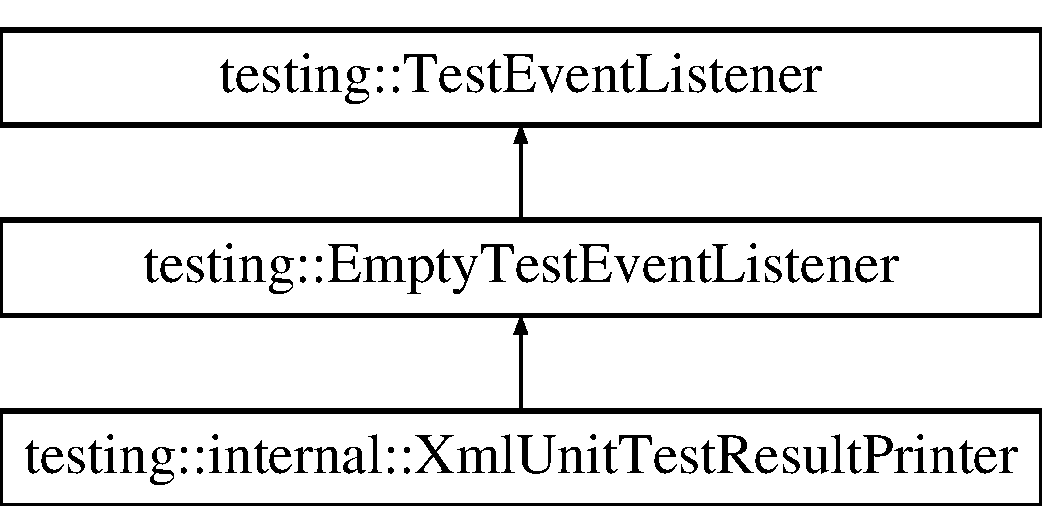
\includegraphics[height=3.000000cm]{classtesting_1_1internal_1_1XmlUnitTestResultPrinter}
\end{center}
\end{figure}
\subsection*{Membros públicos}
\begin{DoxyCompactItemize}
\item 
\hypertarget{classtesting_1_1internal_1_1XmlUnitTestResultPrinter_afdaf88e6764c18ce0dcc3733d7a06e31}{{\bfseries Xml\-Unit\-Test\-Result\-Printer} (const char $\ast$output\-\_\-file)}\label{classtesting_1_1internal_1_1XmlUnitTestResultPrinter_afdaf88e6764c18ce0dcc3733d7a06e31}

\item 
\hypertarget{classtesting_1_1internal_1_1XmlUnitTestResultPrinter_a2ae986dd2f4f2aed31cc6f3bc8c56898}{virtual void {\bfseries On\-Test\-Iteration\-End} (const \hyperlink{classtesting_1_1UnitTest}{Unit\-Test} \&unit\-\_\-test, int iteration)}\label{classtesting_1_1internal_1_1XmlUnitTestResultPrinter_a2ae986dd2f4f2aed31cc6f3bc8c56898}

\end{DoxyCompactItemize}


A documentação para esta classe foi gerada a partir do seguinte ficheiro\-:\begin{DoxyCompactItemize}
\item 
src/gtest.\-cc\end{DoxyCompactItemize}

%--- End generated contents ---

% Index
\newpage
\phantomsection
\addcontentsline{toc}{chapter}{Índice}
\printindex

\end{document}
